\documentclass[a4paper]{report}
\usepackage{float}
\usepackage{verbatim}
\usepackage[utf8]{inputenc}
\usepackage[italian]{babel}
\usepackage{amsmath}
\usepackage{amsbsy}
\usepackage{amsfonts}
\usepackage{amssymb}
\usepackage{graphicx}
\usepackage[left=2cm,right=2cm,top=2cm,bottom=2cm]{geometry}
\usepackage{xcolor}
\usepackage{amsthm}
\usepackage{mhchem}
\usepackage[hypertexnames=false]{hyperref}
\usepackage{nameref}
\usepackage{multicol}
\usepackage{framed}
\usepackage{braket}
\usepackage[framemethod=TikZ]{mdframed}
\usepackage{thmtools}
\usepackage[makeroom]{cancel}

% figure support
\usepackage{import}
\usepackage{xifthen}
\pdfminorversion=7
\usepackage{pdfpages}
\usepackage{transparent}
\usepackage{calc}
\newcommand{\incfig}[1]{%
	\def\svgwidth{\columnwidth}
	\import{./figures/}{#1.pdf_tex}
}
\newcommand{\bs}{\boldsymbol}
\newcommand{\numberset}{\mathcal}
\renewcommand{\L}{\numberset{L}}
\renewcommand{\[}{\begin{equation}}
\renewcommand{\]}{\end{equation}}

\renewcommand{\theequation}{\thesection.\arabic{equation}}
\counterwithin*{equation}{section}

% title setup
\usepackage{xifthen}
\makeatother
\def\@lez{}%
\newcommand{\lez}[3]{
    \ifthenelse{\isempty{#3}}{%
        \def\@lez{Lezione #1}%
    }{%
        \def\@lez{Lezione #1: #3}%
    }%
    \section{\@lez}
    \marginpar{\small\textsf{\mbox{#2}}}
}
\makeatletter

%fatto
\newcounter{fact}[section]\setcounter{fact}{0}
\renewcommand{\thefact}{\arabic{section}.\arabic{fact}}
\newenvironment{fact}[2][]{%
\refstepcounter{fact}%
\ifstrempty{#1}%
{\mdfsetup{%
frametitle={%
\tikz[baseline=(current bounding box.east),outer sep=0pt]
\node[anchor=east,rectangle,fill=blue!20]
{\strut Fatto~\thefact};}}
}%
{\mdfsetup{%
frametitle={%
\tikz[baseline=(current bounding box.east),outer sep=0pt]
\node[anchor=east,rectangle,fill=blue!20]
{\strut Fatto~\thefact:~#1};}}%
}%
\mdfsetup{innertopmargin=10pt,linecolor=blue!20,%
linewidth=2pt,topline=true,%
frametitleaboveskip=\dimexpr-\ht\strutbox\relax
}
\begin{mdframed}[]\relax%
\label{#2}}{\end{mdframed}}

%definizione
\newcounter{defn}[section]\setcounter{defn}{0}
\renewcommand{\thedefn}{\arabic{section}.\arabic{defn}}
\newenvironment{defn}[2][]{%
\refstepcounter{defn}%
\ifstrempty{#1}%
{\mdfsetup{%
frametitle={%
\tikz[baseline=(current bounding box.east),outer sep=0pt]
\node[anchor=east,rectangle,fill=green!20]
{\strut Definizione~\thedefn};}}
}%
{\mdfsetup{%
frametitle={%
\tikz[baseline=(current bounding box.east),outer sep=0pt]
\node[anchor=east,rectangle,fill=green!20]
{\strut Definizione~\thedefn:~#1};}}%
}%
\mdfsetup{innertopmargin=10pt,linecolor=green!20,%
linewidth=2pt,topline=true,%
frametitleaboveskip=\dimexpr-\ht\strutbox\relax
}
\begin{mdframed}[]\relax%
\label{#2}}{\end{mdframed}}


\author{Edoardo Gabrielli}
\title{Appunti di Struttura della Materia}


\begin{document}
\maketitle
\clearpage
\tableofcontents
%\clearpage
\chapter{Termodinamica}
\lez{1}{17-02-2020}{}
\subsection{Introduzione ed argomenti}%
\paragraph{Informazioni sul professore}%
Professore: Alessandro Tredicucci. Ricevimenti sotto richesta Mail (tipicamente il prof è in ufficio nel pomeriggio), ufficio 33 al primo piano.
\paragraph{Informazioni sul corso}%
Il corso spiega proprietà macroscopiche della materia in funzione di proprietà microscopiche. Il nome adatto sarebbe "stati della materia", visto il forte legame del corso con le nozioni di meccanica quantistica basilari. \\
Parleremo di gas perfetti e li useremo per modellizzare proprietà di sistemi fisici più complessi.\\
Le basi che acquisiremo con i gas perfetti ci saranno poco utili nello studio dei liquidi, quest richiederà un altro approccio (e verrà trattata meno).\\
\paragraph{Struttura del corso}%
\begin{itemize}
	\item Gas perfetti $\implies$ gas reali $\implies$ Conducibilità termica.
	\item Solidi. 
	\item Liquidi.
	\item Interazione Radiazione-Materia.
	\item Laser.
\end{itemize}
\paragraph{Libri di testo}%
Il libro di testo scelto è il \textit{David Goldstein: State Of Matter}, contiene tutti gli argomenti trattati nel corso.\\ 
In alternativa c'è il  \textit{Pathria: Statistical Mechanics} oppure \textit{Rimondo: Lezioni di struttura della materia} (attenzione agli erroretti nel testo). Dall'ultimo si prende la parte di Interazione Radiazione-Materia.\\ 
La parte dei solidi viene presa dall' \textit{Ashcroft-Mermin: Solid State Physics} e per approfondire quest'ultima c'è il \textit{Massani Crassano: Fisica dello stato solido} avente molte nozioni di Teoria dei gruppi.\\
Per la parte dei Liquidi: \textit{Marshay e Tosy??} (specifico per Liquidi), si trovano comunque le dispense della prof. Tozzini su e-learning.\\
In ogni caso tenere d'occhio il registro: il prof mette le "Reference" di ogni lezione in modo preciso.\\
E possibile sostituire una parte dell'esame con un seminario: ti prepari un argomento (es. struttura a bande del grafene) e poi lo discuti all'esame.
\paragraph{Esami}%
Le sessioni sono piazzate a fine maggio, giugno, luglio, settembre, ottobre (ti iscrivi e puoi farlo fino a natale), gennaio e febbraio. \\
La modalità di esame è: nella data prestabilità (su valutami) inizia l'appello che dura una settimana o dieci giorni.\\
Al momento dell'iscrizione è necessario scrivere nelle note la data (incluso mattina o pomeriggio) in cui vorremmo fare l'esame, se ti scordi di scrivere nella nota ripeti l'iscrizione. Se la richiesta non è soddisfabile si va in ordine di iscrizione, la lista degli iscritti arriverà per E-mail. In caso di imprevisti è necessario accordarsi con i colleghi per i cambi. L'esame può essere ripetuto a raffica, senza pregiudizi.\\
L'esame è un orale di un'ora: Si parla di due argomenti "ortogonali" del corso (una domanda può essere sostituita dal seminario usando Slide, ogni slide può essere madre di domande atroci). È richiesta la  capacità di applicare quanto visto a lezione e il significato fisico dei risultati ottenuti a lezione, non le rigorose dimostrazioni. \\
Può capitare che vengano chiesti argomenti non visti al corso ma ottenibili ragionando su cose affrontate. 
\begin{center}
	"L'esame è una discussione amichevole di fisica tra fisici :)" \quad \quad Cit. A. Tredicucci
\end{center}
Che succede se non ricordo un argomento dei due chiesti in sede di esame? Si cambia domanda e si parte un voto massimo ribassato: 24-25.\\
È fortemente consigliato dare prima Meccanica Quantistica di Struttura della materia per avere una migliore comprensione degli argomenti trattati ed una maggiore sicurezza in sede di esame.\\
Come bocciare l'esame? Non sapere le distribuzioni statistiche: Boltzmann, Fermi-Dirac, Bose-Einstein con relativi disegni (non fare studio di funzione all'esame per il disegno, va saputo e basta).

\subsection{Assunzioni della termodinamica di Boltzmann}
Come introdotto sopra uno degli scopi del corso è quello di collegare il mondo macroscopico a quello microscopico, per far questo è necessario riprendere i concetti principali di Termodinamica Statistica.
\footnote{Tale campo è quello di Boltzmann e del suo allievo, entrambi si sono suicidati dopo la fama.}\\
Riallacciamoci subito ai concetti di Meccanica Quantistica: supponiamo di avere un sistema con N particelle, possiamo calcolare gli stati di queste particelle passando dalla Hamiltoniana di ognuna di loro. \\
Ottenuto il set di stati possiamo dire che il nostro sistema si troverà sicuramente in uno di questi. Ma come mettiamo in relazione questi stati con la struttura macroscopica della materia?

\paragraph{Esempio: Particelle libere nella scatola}%
Prendiamo una scatola di lato L contenente N particelle non interagente. 
\begin{figure}[H]
    \centering
    \incfig{scatola-l3}
    \caption{Scatola di lato L}
    \label{fig:scatola-l3}
\end{figure}
Ogni particella avrà energia:
\begin{align}
	\epsilon^{\left(i\right)}_{q}=\frac{p_{\left(i\right)}^2}{2m}=\frac{\hbar^2q_{\left(i\right)}^2}{2m}\quad\quad\left(\text{con } \ i = 1 \ \ldots \ N
	\quad \text{e}\quad q^2 = q^2_{x}+ q^2_{y}+q^2_{z} \right)
 .\end{align}
Prendiamo delle condizioni al contorno periodiche per la funzione d'onda:
\[
	 e^{iq_{x}\left( x+l \right) } = e^{q_{x}x} \implies e^{iq_{x}L} = 1
.\] 
Quindi $q_{x} = \left( 2\pi / L \right) l_{x}$, $l_{x} = 0, 1, \ldots N$. Quindi dato il sistema di N particelle di energia totale E avremo un numero estremamante elevato di combinazioni di stati quantistici che possono avere una tale energia:
\begin{align}
	E = \sum_{n=1}^{N} \epsilon_{q}^{\left(i\right)}
.\end{align}
Il nostro obbiettivo è scrivere l'Hamiltoniana con i seguenti criteri:
\begin{itemize}
	\item Particelle non interagenti.
	\item Sistema in grado di passare da uno stato ad un altro \footnote{ad esempio interagendo con le pareti del contenitore o assumendo che gli stati non siano autostati perfetti}.
\end{itemize}
Supponiamo che il sistema sia inizialmente isolato ad una certa energia E e volume $V=L^3$, ci chiediamo quale sia lo stato microscopico in cui si trova.\\
In linea di principio non è possibile colmare questo dubbio: lo stato dipenderà dall'evoluzione temporale del materiale e questa non può sempre esser nota.\\
Per poter caratterizzare meglio la situazione ci servono delle ipotesi:
\begin{itemize}
	\item Se aspettiamo un tempo sufficientemente lungo le condizioni iniziali sono irrilevanti (perdita di memoria del sistema o equilibrio termodinamico).
	\item Se il sistema ha raggiunto l'equilibrio tutti i microstati sono equiprobabili.
\end{itemize}
\paragraph{Apparente contraddizione} %
Con le due ipotesi sopra sembrerebbe che lo stato in cui tutta l'energia E sta in una particella è egualmente probabile allo stato in cui tutte le particelle hanno la stessa energia. \\
In realtà la probabilità di ottenere uno dei due casi è la stessa, soltanto che il numero dei microstati in cui ogni particella ha una energia di circa $E / N$ è molto maggiore del numero dei microstati in cui una particella ha tutta l'energia.\\
Cerchiamo di costruire un metodo per trovare le configurazioni "più probabili" (più popolate), queste ci consentiranno di trovare le proprietà macroscopiche del materiale. Ci serve, in fin dei conti, solo un metodo per contare. 
\subsection{Entropia}%
Boltzmann introduce il concetto di entropia a partire dal numero di microstati $\Gamma$ per un sistema (noti E, N, V). La sua definizione è:
\begin{defn}[Entropia]{def:Entropia}
	\[
	S = k\cdot \ln\Gamma
	.\] 
	con $k = 1.38 \cdot 10^{-23} J\cdot K^{-1}$ costante di Boltzmann.\\
\end{defn}
Visto che $\Gamma$ dipende da V e N possiamo qundi scrivere che $S = S\left( V, N \right)$. \\
Per queste definizioni è necessario l'equilibrio, altrimenti $\Gamma$ sarebbe solo un sottoinsieme degli stati possibili dipendente dalla evoluzione temporale del sistema.\\
Al crescere dell'energia E cresce anche S: se aumento l'energia ho più modi di distribuire l'energia all'interno degli stati quantici. 
\begin{center}
$\Gamma$ è una funzione monotona nell'energia $\implies$ S è monotona nell'energia.
\end{center}
Possiamo quindi scrivere $S = S(V,E,N)$, oppure invertire la relazione (vista la monotonia in E) per esprimere $E = E(S,V,N)$.\\ 
Se l'energia è finita possiamo farne una variazione infinitesima ed ottenere gli importanti potenziali termodinamici.
\subsection{Potenziali termodinamici}%
\[
	dE = \left.\frac{dE}{dS}\right|_{V,N}ds + \left.\frac{\mbox{d} E}{\mbox{d} V} \right|_{S,N}dV + \left.\frac{\mbox{d} E}{\mbox{d} N} \right|_{S,V}dN\\
.\]
\begin{align}
	\left.\frac{\mbox{d} E}{\mbox{d} S}\right|_{V,N}= \ \ T&
	&\left.\frac{\mbox{d} E}{\mbox{d} N}\right|_{S,V} = \ \ \mu& 
	&\left.-\frac{\mbox{d} E}{\mbox{d} V} \right|_{S,N} = \ \ P&
\end{align}
Queste relazioni sono all'equilibrio (a meno che non venga specificata una perturbazione simile al campo elettrico, in qui troveremo comunque soluzioni stazionarie).
\subsection{Potenziale chimico $\mu$}%
Il potenziale chimico è la variazione dell'energia del sistema all'aumentare del numero di particelle.\\
Saremmo portati a pensare che tale valore debba essere positivo in realtà è generalmente negativo: è la variazione di energia a \textit{Volume ed Entropia} costante, se l'entropia è costante allora resta costante anche il numero totale di configurazioni possibili. Per mantenere costante quest'ultimo devo diminurire necessariamente l'energia, da cui il fatto che esso sia negativo.
\footnote{Può essere positivo quando il sistema non può diminuire la sua energia (fermioni a bassa temperatura, grazie al principio di esclusione di Pauli).}

\lez{2}{19-02-2020}{}
Nella scorsa lezione abbiamo introdotto i \textit{sistemi all'equilibrio} (con le relative due ipotesi di lavoro), l'entropia ed i potenziali termodinamici.\\
Concentriamoci adesso su una delle equazioni dei potenziali termodinamici: quella della temperatura.
\subsection{Temperatura}
Abbiamo visto nella scorsa lezione che \[
	T = \left.\frac{\partial E}{\partial S} \right|_{V,N}
.\] 
Cerchiamo di capire il significato fisico della quantità a destra nella equazione.\\
La temperatura ci permette di valutare la possibilità che un corpo scambi energia con altri sistemi.\\
Prendiamo due sistemi isolati:\\
\begin{figure}[H]
    \centering
    \incfig{due-sistemi-isolati}
    \caption{Due sistemi isolati}
    \label{fig:due-sistemi-isolati}
\end{figure}
\noindent Dove $\Gamma_{i}$ è il numero di configurazioni possibili (microstati) di ciascun sistema.\\
Il numero totale di configurazioni possibili quando i due corpi sono staccati sarà (semplici regole di probabilità):
\[
	\Gamma_{T} = \Gamma_1\cdot  \Gamma_2
.\] 
L'energia totale invece:
\[
	E_{T}= E_1+E_2
.\] 
Mettiamo adesso a contatto i due sistemi: la temperatura iniziale dei due sistemi sarà indice del flusso di energia che scorre tra questi ultimi. Ad esempio se non c'è flusso di energia se le due temperature sono le stesse. 
\begin{figure}[H]
    \centering
    \incfig{sistemi-collegati}
    \label{fig:sistemi-collegati}
\end{figure}
\noindent Ipotizziamo che dopo un tempo $t$ stacchiamo nuovamente i corpi, vogliamo vedere cosa avviene a $\Gamma_{T}$ dopo la separazione una volta raggiunto un nuovo equilibrio. Per generalità diciamo che alla fine del processo tutte le variabili di stato elencate in \hyperref[fig:due-sistemi-isolati]{Figura 2} sono primate (esempio: $T_1'$).\\
Prendiamo ad esempio l'energia finale dei due sistemi: $E_1', \ E_2'$, entrambe avranno una certa probabilità di esistere quando i sistemi sono nuovamente staccati. Tale probabilità sarà proporzionale al numero di microstati che esistono con tali energie per ciascun sistema: $\Gamma_1', \ \Gamma_2'$.\\ 
Quindi la probabilità di trovare il primo sistema con l'energia $E_1'$ ed il secondo con l'energia $E_2'$ sarà proporzionale a $\Gamma_1'\cdot \Gamma_2'$.\\
Quindi quando li stacco l'energie più probabili sono quelle che massimizzano il prodotto tra i microstati corrispettivi: $\Gamma_1'\cdot \Gamma_2'$.\\
L'entropia del sistema sarà allora:
\[
	S' = k \ln \Gamma_1'\cdot \Gamma_2'
.\] 
O in alternativa:
\[
	S' = S_1' + S_2'
.\] 
Come conseguenza della prima equazione l'entropia dopo la separazione sarà la massima possibile!\\
Supponiamo che vi sia una differenza di energia tra istante finale ed istante iniziale per ogni sistema, possiamo esprimerla come:
\begin{align}
	&\delta E_1= E_1'-E_1 = T_1 \delta S_1\\
	&\delta E_2 = E_2' - E_2 = T_2 \delta S_2
.\end{align}
L'ultima uguaglianza deriva dal fatto che possiamo considerare variazioni infinitesime e applicare la prima equazione di questa sezione.\\
Essendo tutto isolato dall'esterno si ha anche che:
\[
	\delta \left( E_1 + E_2 \right) = 0 \implies \delta E_1 = - \delta E_2
.\] 
E sostituendo con quanto ottenuto sopra:
\[
	T_1 \delta S_1 + T_2 \delta S_2 = 0
.\] 
Cerchiamo adesso la configurazione in cui non c'è stato flusso di energia durante il contatto: tale configurazione sarà quella per cui l'entropia prima del contatto era già su un massimo. Di conseguenza in questa situazione:
\[
	\delta S = \delta S_1 + \delta S_2 = 0
.\] 
Di conseguenza non vi è flusso di energia proprio quando le temperature dei due corpi erano inizialmente le stesse:
\[
	T_1 = T_2
.\] 
Allo stesso modo possiamo imporre $\delta S\ge 0$ e vedere che in tal caso $\delta E_{i}$ sarà positivo per un corpo e negativo per l'altro e quindi dedurre una disuguaglianza tra le due temperature iniziali.

\begin{framed}
\noindent \textbf{Nota}: \\
Potremmo fare gli stessi ragionamenti
\begin{itemize}
	\item per la pressione: prendiamo due sistemi isolati e li mettiamo a contatto, adesso questi due potranno scambiare volume.
	\item per il potenziale chimico $\mu$: prendiamo due sistemi isolati e mettiamoli a contatto, apriamo poli tra le membrane per permettere lo scambio di sole particelle.
\end{itemize}
\end{framed}
\noindent 
Se fossimo in grado di calcolare il $\Gamma$ saremmo in grado di calcolare $E\left( S \right)$, di conseguenza potremmo sapere tutto del nostro sistema, infatti:
\[
	T\left( S,V,N \right)  = \left.\frac{\partial E}{\partial S} \right|_{V,N}
.\] 
\[
	- P \left( S,V,N \right) = \left.\frac{\partial E}{\partial V} \right|_{S,V}
.\] 
Dalla prima possiamo ricavare $S\left( T \right)$ ed inserirla nella seconda ottenendo $P\left( T,V,N \right)$. Nel caso dei gas perfetti si ottiene proprio l'equazione di stato $P\cdot V = nRT$.\\
Il metodo esposto, per quanto ragionevole, non è affatto pratico. Tuttavia ci dà molte informazioni su come procedere operativamente in varie situazioni, ad esempio se abbiamo il numero di particelle ci bastano due variabili per descrivere il sistema (ad esempio V e T).\\ 
\paragraph{Indeterminazione dell'energia}%
Nel ragionamenti per mostrare che la temperatura si comporta effettivamente come ci aspettiamo ci siamo persi qualche passaggio.\\ 
Siamo partiti da due sistemi all'equilibrio con ciascuno le sue variabili di stato, anche solo considerando $T_1= T_2$ (quindi mettendoli a contatto anche dal punto di vista macroscopico non succede niente) dopo "l'interazione" ci siamo persi la variabile di stato energia: non sarà più unicamente determinata per i due corpi ma avrà una distribuzione (che massimizza il prodotto $\Gamma_1\cdot \Gamma_2$), quindi qualcosa è cambiato!\\ 
Siamo quindi passati da energie ben definite e fissate a quelle più probabili: abbiamo introdotto una indeterminazione.\\
Fortunatamente per sistemi macroscopici la configurazione che massimizza l'entropia è più probabile di tutte le altre configurazioni messe insieme, questo giustifica il nostro ragionamento ed il fatto che consideriamo le energie finali unicamente definite.\\
In realtà abbiamo indeterminazione anche nell'energia di partenza, questa non viene dal nulla: è stata passata ai corpi in qualche istante molto precedente a quello considerato. Quindi anche le energie iniziali non sono in realtà semplici numeri ma distribuzioni, proprio come le energie finali.\\
Abbiamo inoltre una ulteriore indeterminazione nel conto del $\Gamma$: il fatto che il nostro sistema non ha nemmeno una energia ben definita per via della meccanica quantistica. \\
Abbiamo dato come necissità che il nostro sistema possa passare da uno stato ad un altro, anche se le particelle non interagiscono, allora il nostro microstato quantistico del sistema ha un tempo di vita media $\tau$, quindi per il principio di indeterminazione:
\[
	\delta E \gtrsim \frac{\hbar}{\tau}
.\] 
Anche l'energia stessa avrà quindi una indeterminazione aggiuntiva dovuta alla meccanica quantistica, questo comporta un problema nel calcolo di $\Gamma$.
Fortunatamente le incertezze introdotte dalla meccanica quantistica nei conti termodinamici non contano molto grazie alla definizione di entropia:
\[
	S = k \ln\Gamma
.\] 
Il numero di configurazioni entra con un logaritmo, sbagliando di un'ordine di grandezza su $\Gamma$ sbaglio di un fattore misero il conto dell'entropia.\\
C'è un altro modo per aggirare il problema dell'indeterminazione dell'energia (utile perchè maggiormente applicabile a sistemi non isolati \footnote{tratteremo in genere sistemi che sono all'equilibrio termico con il mondo che li circonda}).
Sarà utile a questo scopo la funzione 
\[
	\rho_{E} = \frac{\mbox{d} \Gamma}{\mbox{d} E} 
.\] 
Ovvero la densità di stati in energia, piuttosto che $\Gamma$. La funzione $\rho_{E}$ ci dice quanti stati ci sono per unità di energia.
\begin{framed}
\noindent \textbf{Nota}: \\
Stiamo implicitamente assumendo che l'entropia S non sia nulla: in tal caso avremmo un solo stato accessibile al sistema, il sistema si trova necessariamente nello stato fondamentale.
Analogamente se il sistema ha temperatura nulla, in tal caso il sistema non può cedere energia al mondo esterno, quindi è necessariamente nel fondamentale.
\end{framed}
\noindent 
Torniamo ai nostri due oggetti di temperatura diversa, il sistema è un genere fuori equilibrio globalmente ma possiamo considerarlo composto (localmente) a tanti piccoli sistemi che sono localmente all'equilibrio. Per questi sistemi locali sono ben definiti i concetti di entropia, temperatura, ecc\ldots
\begin{framed}
\noindent \textbf{Nota}: \\
Il concetto di equilibrio non è una configurazione fissa e immutabile: il sistema, raggiunto l'equilibrio, sarà soggetto a fluttuazioni attorno ad una configurazione media. Il concetto di equilibrio è quindi un concetto dinamico.
\end{framed}
\noindent 
\subsection{Principi classici della termodinamica sotto l'ottica statistica}
Vediamo adesso il rapporto tra gli argomenti visti ed i principi classici della termodinamica.
\paragraph{Principio 1}%
La variazione di energia è data dal calore scambiato dal sistema più il lavoro fatto dal sistema.
\[
	dE = dQ + dL
.\] 
Affrontiamo adesso una \textit{Trasformazione adiabatica}.
Prendiamo il classico esempio del pistone:
\begin{figure}[H]
    \centering
    \incfig{cilindro-con-pistone}
    \caption{Cilindro con pistone}
    \label{fig:cilindro-con-pistone}
\end{figure}
\noindent Supponiamo di spostare il pistone del tratto infinitesimo $\Delta x$, questo richiede una forza $F$. Il lavoro fatto sul sistema sarà 
 \[
	dL = F \Delta x
.\] 
d'altra parte la pressione è definita da
\[
	P = \frac{F}{A}
.\] 
Quindi 
\[
	dL = P\left( A \Delta x \right) = -PdV
.\] 
Se il sistema è rimasto isolato per tutta la durata della spinta del pistone si ha che $dQ=0$, quindi:
\[
	\left.\frac{\mbox{d} E}{\mbox{d} V}\right|_{Q} = -P
.\] 
Confrontandolo con il differenziale dell'energia:
\[
	dE = TdS - P dV + \mu dN
.\] 
Sembrerebbe che una trasformazione adiabatica sia una trasformazione isoentropica \footnote{dN non varia perchè ipotizziamo che il cilindro non abbia perdite di particelle dalle pareti}. Diamone una interpretazione statistica.\\
Prendiamo un sistema che si trova in un macrostato con energia E, entropia S, N, V ecc\ldots e scriviamo i livelli energetici delle sue singole molecole, ad esempio:
\begin{figure}[H]
    \centering
    \incfig{distribuzione-livelli-molecole}
    \label{fig:distribuzione-livelli-molecole}
\end{figure}
\noindent
Se facciamo la trasformazione adiabatica molto lentamente quello che facciamo è semplicemente spostare i livelli verso l'alto (aumentiamo l'energia di ogni singolo livello), senza modificarne la struttura.
\begin{figure}[H]
    \centering
    \incfig{livelli-energetici-alzati}
    \label{fig:livelli-energetici-alzati}
\end{figure}
\noindent
Quindi il numero di livelli ed il numero di configurazioni possibile resta lo stesso, da cui la conservazione dell'entropia iniziale.\\
Vediamo adesso il processo speculare: una trasformazione con il \textit{solo scambio di calore}. \\
Non essendoci lavoro sul sistema si ha, dal primo principio:
\[
	dE = dQ = TdS
.\] 
\paragraph{Principio 2}%
Il sistema fuori equilibrio termodinamico tende ad evolvere verso una configurazione che massimizza l'entropia.
\paragraph{Principio 3}%
Tutti i corpi a temperatura uguale zero hanno entropia nulla.\\
\begin{framed}
\noindent \textbf{Nota}: \\
Temperatura nulla significa che il nostro sistema non è in grado di cedere energia ad un altro sistema, quindi il sistema si trova nello stato fondamentale (minima energia) e per definizione in questo stato l'entropia è nulla. Ma entropia nulla significa che $\Gamma=1$, questo vuol dire che lo stato fondamentale non può essere degenere.
\end{framed}
\noindent 

\paragraph{Estensione del concetto di variabili termodinamiche}%
Partiamo da un sistema con un numero di particelle fissato, l'energia diventa una semplice funzione di S e V
\[
	dE = TdS - PdV
.\] 
\begin{framed}
\noindent \textbf{Nota}: \\
Nella equazione precedente abbiamo due termini accoppiati a destra: la temperatura è accoppiata con l'entropia e la pressione con il volume.\\
Le grandezze così accoppiate come quelle sopra sono dette in termodinamica \textit{Grandezze Coniugate} e tipicamente sono una estensiva ed una intensiva.
\begin{itemize}
	\item Grandezza estensiva: raddoppiando le dimensioni del sistema raddoppia anche la grandezza (Volume, Entropia).
	\item Grandezza intensiva: Grandezze che non ci diconon nulla sulla dimensione del sistema (Temperatura, Pressione).
\end{itemize}
\end{framed}
\noindent 
Se riusciamo a scrivere $E\left( S,V,N \right)$ abbiamo risolto il problema termodinamico, (S,V, N) sono dette in generale le variabili proprie del sistema. Nel nostro caso ci bastano (S,V) perchè abbiamo fissato il numero di particelle. \\
Potremmo dire lo stesso con (T,V)? No, non sono sufficienti, non hanno abbastanza informazioni.\\
Abbiamo allora un problema sperimentale: l'entropia non è facilmente misurabile, dobbiamo definire l'energia a partire da oggetti che possano essere misurati con semplicità. Sulla base di questo problema nascono gli altri potenziali termodinamici. 
\subsection{Utili potenziali termodinamici}
\paragraph{Energia libera di Halmotz}%
\[
	F = E - TS
.\] 
Differenziando questa quantità si ottiene:
\[
	dF = -SdT - PdV
.\] 
Quindi F = $F\left( T,V \right)$ e si ricava facilmente che:
\[
	F\left( T,V \right) \implies 
	\begin{cases}
	S = - \left.\frac{\partial F}{\partial T} \right|_{V} \\ 
		\\
	P = - \left.\frac{\partial F}{\partial V} \right|_{T}
	\end{cases}
.\] 
Questa è molto utile per studiare sistemi non isolati e mantenuti ad esempio a temperatura T.\\
Si può inoltre verificare che 
\[
	\left.\delta F\right|_{T} = -P \left.\delta V\right|_{T} = \delta L
.\] 
F ci toglie il problema di trovare l'entropia del sistema e capire come è legata all'energia (che è complicato). Sfortunatamente con F ci perdiamo la connessione con il numero di microstati, quindi questa legge è utile al livello macroscopico ma è complicato poi trarne conclusioni a livello microscopico.
\paragraph{Energia libera di Gibbs}%
\[
	\phi = F + PV
.\] 
\[
	d\phi = -SdT + VdP
.\] 
Quindi si ricavano le relazioni:
\begin{align}
	&S = -\left.\frac{\partial \phi}{\partial T}\right|_{P}\\
	&V = \left.\frac{\partial \phi}{\partial P} \right|_{T}
.\end{align}
Questa è utile se si va a studiare l'equilibrio tra fasi diverse (esempio: evaporazione di un liquido: Avremo curve caratteristiche in pressione quando andiamo ad imporre che il $\phi$ del liquido sia uguale al $\phi$ del gas).\\
\paragraph{Entalpia}%
\[
	W = \phi + TS
.\] 
\[
	dW = TdS + VdP
.\] 
Quindi si hanno le relazioni:
\begin{align}
	&T = \left.\frac{\partial W}{\partial S}\right|_{P}\\
	&V = \left.\frac{\partial W}{\partial P} \right|_{S}
.\end{align}
e si ha anche:
\[
	 \left.\delta W\right|_{P} = T \left.\delta S\right|_{P}= \left.\delta Q\right|_{P}
.\] 
In questa abbiamo uno scambio di calore a pressione costante, è nota come funzione del calore.\\
Alle volte è comodo non passare direttamente dai potenziali termodinamici ma fare delle derivate seconde incrociate, ad esempio:
\[
	\left.\frac{\partial P}{\partial T} \right|_{V}=
	\left.\frac{\partial }{\partial T} \left.\left( -\frac{\partial F}{\partial V}\right|_{T}  \right) \right|_{V}
	= -\left.\frac{\partial }{\partial V}\left(  \left.\frac{\partial F}{\partial T} \right|_{V}  \right) \right|_{T} =
	-\left.\frac{\partial S}{\partial V} \right|_{T} 
.\] 
E in questo modo possiamo trovare delle utili relazioni dette \textit{Relazioni di Maxwell}.\\
Effettuando una \textit{Trasformazione di scala} (vedi Goldstein) si conclude che:
\[
	d\mu = - \frac{S}{N}dT + \frac{V}{N}dP 
.\]
Quindi abbiamo che:
\[
	\phi\left( P,T \right) = \mu N
.\] 
e possiamo concludere un'altra importante relazione tra i potenziali termodinamici:
\[
	\left.\delta E\right|_{S,V} = \left.\delta F\right|_{T,V} = \left.\delta \phi\right|_{T,P} = \left.\delta W\right|_{S, P}
.\] 
\paragraph{Potenziale di Landau}%
\[
	\Omega = F - \mu N
.\] 
\[
	d\Omega = -SdT - PdV - Nd\mu
.\] 
Si dimostra anche che $\Omega = -PV$ e che:
\[
	\left.\delta \Omega\right|_{T,V,\mu} = \left.\delta E\right|_{S, V, N}= \ldots
.\] 
Rivediamo adesso il nostro principio variazionale e la nostra posizione di equilibrio studiando un caso specifico:
\paragraph{Corpo immerso in un bagno termico}%
Consideriamo un sistema immerso in un bagno termico (un sistema con caratteristiche tali da rimanere imperturbato a livello energetico dal contatto con il sistema immerso al suo interno).
\begin{figure}[H]
    \centering
    \incfig{bagno-termico}
    \caption{Bagno termico}
    \label{fig:bagno-termico}
\end{figure}
\noindent
Tutto quanto è mantenuto alla temperatura T.\\
Per il bagno termico possiamo scrivere che:
\[
	dE' = TdS'
.\] 
Sappiamo inoltre che il tutto è isolato, quindi:
\[
	\delta\left( E+E' \right) = 0 \implies
	\delta E + \delta E' = 0
.\]
Per quanto visto sopra abbiamo:
\[
	\delta E + T\delta S' = 0 
.\] 
quindi \[
	\delta S' = - \frac{\delta E}{T}
.\] 
Il nostro sistema inizialmente era fuori equilibrio (tutto: sistemino + bagno termico) allora avremo che $\delta S \ge 0$:
\[
	\delta S + \delta S' \ge  0
.\] 
E sostituendo l'equazione ricavata prima:
\[
	T\delta S - \delta E \ge 0 \implies
	\delta \left( E- TS \right) \le 0
.\] 
Ma $E-TS = F$, quindi abbiamo che: 
\[
	\delta F \le 0
.\] 
Quindi per un sistema fuori equilibrio immerso in un bagno termico la condizione di equilibrio è quella che minimizza l'energia libera di Halmotz.
Nel caso in cui può variare anche N si avrebbe più in generale che:
\[
	\Omega = F - \mu N \implies \delta \Omega \le  0
.\] 

\subsection{Capacità termica e compressibilità}%
Si arriva alla capacità termica ed alla compressibilità a partire dalle derivate seconde di alcuni potenziali termodinamici:
\[
	C_{V} = T\cdot \left.\frac{\partial S}{\partial T} \right|_{V} = \left.\frac{\partial E}{\partial T} \right|_{V}=
			- T \left.\frac{\partial ^2 F}{\partial T^2 } \right|_{V}
.\] \label{eq:capacita-termica}
\[
	C_{p} = T \left.\frac{\partial S}{\partial T} \right|_{P} = \ldots = - T \left.\frac{\partial ^2 \phi}{\partial T^2} \right|_{P}
.\] 
Analogamente per la compressibilità isoterma o adiabatica:
\[
	k_{P}= -\frac{1}{V} \left.\frac{\partial V}{\partial P} \right|_{T} =
	-\frac{1}{V} \left.\frac{\partial ^2 \phi}{\partial P^2} \right|_{T}
.\] 
\[
	k_{S} = -\frac{1}{V}\left.\frac{\partial V}{\partial P} \right|_{S}=
	\left[ V\cdot \left.\frac{\partial^2 E}{\partial V^2} \right|_{S} \right] ^{-1}
.\] 
Questi sono importanti dal punto di vista pratico: la capacità termica e la compressibilità sono cose che si misurano molto bene.

\lez{3}{21-02-2020}{}
Le grandezze introdotte a fine della scorsa lezione non sono tutte indipendenti tra loro, ci sono delle relazioni che si saranno utili:
\[
	\frac{C_{V}}{T}= \left.\frac{\partial S}{\partial T} \right|_{V}= \left.\frac{\partial S}{\partial P} \right|_{T} \left( \frac{\partial P}{\partial T}  \right) _{V} + \left.\frac{\partial S}{\partial T} \right|_{P}
.\] 
Quindi usando la relazione di Maxwell
\[
	\left.\frac{\partial S}{\partial P} \right|_{T}= - \left.\frac{\partial V}{\partial T} \right|_{P}
\]
Possiamo arrivare alla relazione:
\[
	 \frac{C_{P}- C_{V}}{T}= \left.\frac{\partial V}{\partial T} \right|_{P} \left.\frac{\partial P}{\partial T} \right|_{V}
.\] 
Questa relazione può essere riscritta in anche altri termini considerando la permutazione ciclica delle derivate:
\[
	\left.\frac{\partial V}{\partial T} \right|_{P} \left.\frac{\partial T}{\partial P} \right|_{V} \left.\frac{\partial P}{\partial V} \right|_{T} = -1
.\] 
Per esempio possiamo eliminare una delle variabili per scrivere alcune relazioni che mettono in corrispondenza i calori specifici con la compressibilità:
\[
	C_{P}- C_{V}= TVk_{T} \left[ \left.\frac{\partial P}{\partial T} \right|_{V} \right] ^2 
		= \frac{T}{V k_{T}} \left[ \left.\frac{\partial V}{\partial T} \right|_{P} \right]^2
.\]
\subsection{Segno delle capacità termiche}%
La capacità termica è una quantità sempre positiva. Dal punto di vista intuitivo risulta naturale: se aumento la temperatura di un oggetto sto aumentando l'entropia e di conseguenza anche l'energia \footnote{Nella definizione abbiamo la variazione di energia.}.\\
È comunque possibile dimostrarlo a partire dalle condizioni di equilibrio che abbiamo trovato. 
\paragraph{Dimostrare che la capacità termica e la compressibilità sono sempre positive}%
Consideriamo il seguente sistema:
\begin{figure}[H]
    \centering
    \incfig{cvpositiva}
    \caption{Sistema di due volumi divisi da una membrana immersi in un bagno termico.}
    \label{fig:cvpositiva}
\end{figure}
\noindent
Il sistema è costituito da un gas diviso tra due volumi da una membrana libera di muoversi, il tutto è immerso in un bagno termico a temperatura T. \\
Cerchiamo la condizione di equilibrio del sistema. Abbiam visto che, non essendo il sistema isolato, la funzione da utilizzare è l'energia libera F. La condizione di equilibrio sarà data dal fatto che l'energia libera deve essere in un minimo \footnote{Questo deve essere vero per tutte le variabili da cui dipende l'energia libera}. \\
Visto le caratteristiche del sistema la variazione di volume totale sarà per ogni istante nulla:
\[
	dV_1 + dV_2= 0
.\] 
Cerchiamo adesso la derivata dell'energia libera totale rispetto a $V_1$:
\[
	\frac{\partial F}{\partial V_1} = \frac{\partial \left( F_1+F_2 \right) }{\partial V_1} = \frac{\partial F_1}{\partial V_1} - \frac{\partial F_2}{\partial V_2}= P_1 - P_2 
.\] 
Essendo all'equilibrio la quantità che stiamo calcolando deve essere nulla:
\[
	P_1 = P_2
.\] 
Avendo imposto che sia un minimo la derivata seconda deve essere positiva:
\[
	\frac{\partial ^2 F}{\partial V_1^2} = \frac{\partial }{\partial V_1} \left( P_2-P_1 \right) = - \frac{\partial P_1}{\partial V_1} - \frac{\partial P_2}{\partial V_2} >0
.\] 
Visto che $\frac{\partial P}{\partial V} = -VK_{T}$ (definizione) si ha:
\[
	\frac{1}{K_{T_1}V_1} + \frac{1}{k_{T_2}V_2} >0
.\] 
Se il gas nei due setti è lo stesso allora abbiamo anche che $k_{T_1}$ = $k_{T_2}$
\[
	k_{T} >0
.\] 
Quindi abbiamo ottenuto una proprietà generale: \textit{La compressibilità è sempre positiva}. \\
\begin{framed}
\noindent \textbf{Nota}: \\
Se $k_{T}<0$ ci troveremmo in una buffa situazione, avremmo che è verificata la disequazione:
\[
	\left.\frac{\partial V}{\partial P} \right|_{T}<0 \quad \text{Con $k_{T}$ negativa}
.\] 
Quindi il volume aumenterebbe all'aumentare della pressione \footnote{A temperatura costante!}, non si raggiungerebbe mai un equilibrio perchè il sistema andrebbe ad esplodere occupando tutto l'universo.\\
\end{framed}
\noindent 
Possiamo ripetere quanto fatto con $k_{T}$ per dimostrare che anche la capacità termica deve essere positiva, infatti basta prendere un sistema isolato diviso in due parti
\begin{figure}[H]
    \centering
    \incfig{sistema-isolato}
    \caption{Sistema a due setti isolato termodinamicamente.}
    \label{fig:sistema-isolato}
\end{figure}
\noindent
Sfruttiamo questa volta l'entropia:
\[
	\frac{\partial S}{\partial E_1} = \frac{1}{T_1}- \frac{1}{T_2}
.\] 
Per la conservazione dell'energia del sistema si ha:
\[
	dE_1 + dE_2=0
.\] 
Imponendo l'equilibrio si ha che S è sicuramente in un massimo, quindi facendo passaggi analoghi a sopra si troverebbe banalmente che è necessario $T_1 = T_2$.\\
Se ci concentriamo sulla derivata seconda di S rispetto ad una delle due enrgie invece si ha:
\[
	\frac{\partial }{\partial E_1} \left( \frac{1}{T_1} \right) + \frac{\partial }{\partial E_2} \left( \frac{1}{T_2} \right) =
	-\frac{1}{T_1^2}\frac{\partial T_1}{\partial E_1} -\frac{1}{T_2^2}\frac{\partial T_2}{\partial E_2} = 
	-\frac{1}{C_{V_1}T_1^2}-\frac{1}{C_{V_2}T_2^2} \le 0
.\] 
L'ultima disuguaglianza è dovuta al fatto che S è in un massimo. Se imponiamo che nei due setti vi sia la stessa sostanza allora si conclude anche qui:
\[
	C_{V}>0
.\] 
Notiamo che se $C_{V}$ è positivo a maggior ragione $C_{P}$ è maggiore di zero per via delle relazioni che li legano trovate ad inizio lezione.

\subsection{Transizioni di fase di un sistema}%
\label{sec:transizioni-di-fase}
Prendiamo un generale diagramma di fase di un materiale: un Plot (P,T).
\begin{figure}[H]
    \centering
    \incfig{diagramma-di-fase-generico}
    \caption{Diagramma di fase generico}
    \label{fig:diagramma-di-fase-generico}
\end{figure}
\noindent
Le linee che separano le fasi ci indicano zone in cui due fasi sono in equilibrio tra loro, quindi in queste condizioni varie fasi possono coesistere. \\
Se ad esempio abbiamo fase liquida e solida in una zona di coesistena allora fissata la temperatura sarà fissata automaticamente anche la pressione, essa sarà vincolata su una curva dipendente da T.\\
Tipicamente le curve hanno una "Slope" positiva, i casi in cui questo non è vero sono pochi, vedremo qualche esempo più tardi.\\
\begin{defn}[Punto Triplo]{defn:Punto Triplo}
Il punto in cui coesistono tutte le fasi è detto \textit{punto triplo}.
\end{defn}

\paragraph{Curve di coesistenza}%
Per studiare le zone di coesistenza possiamo possiamo prendere un sistema composto da un recipiente di N atomi dello stesso elemento diviso in due sottosistemi contenente le due fasi: ad esempio liquida e gassosa\\
\begin{figure}[H]
    \centering
    \incfig{sistema-diviso-in-due-fasi}
    \caption{Sistema diviso in due fasi}
    \label{fig:sistema-diviso-in-due-fasi}
\end{figure}
\noindent
È facile immaginare questo sistema: di solito nella separazione di fase varia la densità e quindi la gravità divide spontaneamente i due stai.\\
Per trovare il diagramma di fase a partire da questo sistema supponiamo che la temperatura del sistema sia fissatta, imponiamo le condizioni di equilibrio (F minimo) in funzione del numero di particelle nel recipiente:
\[
	\frac{\partial F}{\partial N_1} = \frac{\partial F}{\partial N_2} 
.\] 
Ma $\frac{\partial F}{\partial N} $ è il potenziale chimico $\mu$ \footnote{Il parametro che ci dice quando due sottosistemi che possono scambiare particelle tra di loro sono all'equilibrio}.
Quindi dobbiamo trovare $\mu_1$ del liquido e $\mu_2$ del gas ed imporre che siano uguali. Visto che $\mu$ è una buona grandezza termodinamica delle variabili (P,T).  Di conseguenza abbiamo fissato una curva (P,T) quando due specie sono all'equilibrio termodinamico.\\
Possiamo inoltre notare che nel punto triplo abbiamo 2 uguaglianze:
\[
	\mu_{\text{solido}}=\mu_{\text{liquido}}= \mu_{\text{gas}}
.\] 
Che individuano anzichè una curva un punto nel piano (P,T), che è compatibile con quanto affermato fin'ora.

\paragraph{Punto Critico}%
La curva disegnata ha un "limite" detto punto critico, oltre il tale non esistono più fase liquida e gassosa ma abbiamo soltanto una unica fase (fluida) e le curve smettono di esistere. 
\begin{figure}[H]
    \centering
    \incfig{punto-critico}
    \caption{Punto critico}
    \label{fig:punto-critico}
\end{figure}
\noindent
Questo punto si osserva perchè non si riesce più ad osservare una transizione di fase: non si ha nessuna discontinuità di grandezze fisiche della sostanza nel sistema.
\begin{framed}
\noindent \textbf{Nota}: \\
In linea di principio possiamo inventarci una trasformazione che porti da gas a liquido senza aver effettuato una transizione di fase passando da sopra le curve del diagramma di fase! 
\end{framed}
\noindent 
Tra lo stato solido e lo stato liquido non ci sono prove sperimentali sul fatto che esista un punto critico. 

\paragraph{Diagramma (P,V)}%
Oltre allo spazio (P,T) possiamo fare anche un diagramma delle fasi nello spazio (P,V). Tipicamente tale diagramma prende la forma:
\begin{figure}[H]
    \centering
    \incfig{diagramma-pv}
    \caption{Diagramma PV}
    \label{fig:diagramma-pv}
\end{figure}
\noindent
Tale grafico è utile per analizzare le zone di coesistenza (quelle in basso, dove non vi sono stati definiti gli stati) che nell'altro grafico erano semplicemente puntiformi.\\
Possiamo vedere come si trasformano le curve isoterme dal grafico (P,T) al grafico (P, V):
\begin{figure}[H]
    \centering
    \incfig{curve-isoterme-pt-pv}
    \caption{curve isoterme PT PV}
    \label{fig:curve-isoterme-pt-pv}
\end{figure}
\noindent

\paragraph{Sistemi particolari}%
Alcuni sistemi non hanno entrambe le slope positive, il classico esempio è l'acqua:
\begin{figure}[H]
    \centering
    \incfig{diagramma-di-fase-dell'acqua}
    \caption{Diagramma di fase dell'acqua}
    \label{fig:diagramma-di-fase-dell'acqua}
\end{figure}
\noindent
In cui la Slope della curva di separazione tra solido e liquido è negativa.\\
Un caso ancora più strano è quello dell'elio:
\begin{figure}[H]
    \centering
    \incfig{diagramma-di-fase-dell'elio}
    \caption{Diagramma di fase dell'elio}
    \label{fig:diagramma-di-fase-dell'elio}
\end{figure}
\noindent
In questo caso abbiamo una curva di coesistenza del gas "normale", ma la curva del solido non incontra mai quella del gas. \\
La cosa più strana è che le fasi liquide sono due: quella standard e quella superfluida.\\
Cerchiamo di capire a cosa è legata la pendenza della curva.
\paragraph{Pendenza delle curve di separazione delle fasi}%
Prendiamo come esempio il caso dell'acqua e mettiamoci in una zona di separazione tra gas e liquido alla temperatura $T_0$ e pressione $P_0$ in una condizione di equilibrio termodinamico:\\
\begin{figure}[H]
    \centering
    \incfig{punto-sulla-separazione-gas-liquido-per-l'acqua}
    \caption{Punto sulla separazione gas-liquido per l'acqua}
    \label{fig:punto-sulla-separazione-gas-liquido-per-l'acqua}
\end{figure}
\noindent
Cambiamo la temperatura di $dT$ infinitesimo, è possibile supporre di essere ancora in uno stato di equilibrio per una variazione sufficientemente piccola \footnote{O comunque che dopo poco tempo il sistema si riassesti all'equilibrio}.\\
per una trasformazione del genere si ha in generale una variazione della pressione ed anche dei potenziali termodinamici, supponiamo che in questo caso la piccola variazione no induca un cambiamento di questi ultimi. In particolar modo non si induce allora una variazione nel potenziale chimico delle due fasi, la cui variazione ricordiamo essere:
 \[
	d\mu=-\frac{S}{N}dT + \frac{V}{N}dP
.\] 
Visto che siamo ancora all'equilibrio $d\mu_1$ = $d\mu_2$, dove il pedice indica lo stato (liquido o gassoso), quindi abbiamo:
\[
	-s_1 dT + v_1 dP = -s_2 dT + v_2 dP
.\] 
Dove si introduce la notazione per ciascuna specie:
\begin{align}
	&s = S/N \quad \text{Entropia per particella}\\
	&v = V/N \quad \text{Volume per particella}
.\end{align}
Notiamo che $v$ è l'inverso del volume.\\
Possiamo allora esprimere la pendenza della curva di separazione tra gli stati nel grafico PT come:
\[
	\frac{\mbox{d} P}{\mbox{d} T} = \frac{s_1-s_2}{v_1-v_2}
.\] 
Che è la relazione di \textit{Klausius-Clapeiron}.\\
Possiamo definire anche un calore latente quando avviene una transizione di fase: 
\begin{defn}[Calore latente]{defn:Calore latente}
\[
	L = T \Delta s = T \left( s_1-s_2 \right) 
.\]
\end{defn}
Che è la quantità di calore per particella da fornire per far avvenire la transizione di fase.\\
Tramite $L$ possiamo scrivere la relazione di Klausius-Clapeiron in modo più compatto:
\begin{fact}[Relazione di Clausius-Klapeiron]{fact:relazione di Clausius-Klapeiron}
\[
	\frac{\mbox{d} P}{\mbox{d} T} = \frac{L}{T\left( v_1-v_2 \right) }
.\] 
\end{fact}
Adesso possiamo capire perchè questa quantità è in generale positiva: ci aspettiamo ad esempio che andando da gas (stato 1) verso il liquido (stato 2) l'entropia ed il volume specifico diminuiscano. Quindi nella relazione sopra numeratore e denominatore sono nella maggior parte dei casi positivi.\\
Per l'acqua la Slope solido-liquido è negativa per il semplice motivo che il ghiaccio è meno denso dell'acqua liquida, questo inverte il segno al denominatore nella equazione sopra.\\
Nel caso dell'elio invece abbiamo una transiozione da solido a superfluido con dei punti in cui la slope è zero. Qui la densità non c'entra: è una questione di entropia. \\
Si ha infatti che il superfluido può avere entropia minore del solido! Questo sarà collegato al Condensato di Bose-Einstein che vedremo.

\subsection{Conteggio degli stati $\Gamma$}%
Preso il sistema con (E,V,N) abbiamo definito l'entropia $S = k \ln\Gamma$, da qui abbiamo costruito tutta la nostra teoria termodinamica partendo dal concetto di equilibrio. Adesso dobbiamo trovare come calcolare il numero di stati associato con le variabili di stato.\\
In linea di principio se avessimo un gas perfetto composto da particelle indipendenti, non interagenti, all'equilibrio termodinamico, senza gradi di libertà interni ecc\ldots potremmo prendere gli stati di una singola particella nella scatola di volume V e vedere come sono distribuite queste N particelle negli stati in modo tale che la loro energia sia complessivamente E.\\
Questo funziona quando abbiamo poche particelle, se abbiamo $10^{23}$ particelle inizia ad essere complicato. \\
Inoltre potrebbero nascere dei problemi dalle indeterminazioni intrinseche dei livelli energetici come abbiamo discusso. \\
Un ulteriore problema è dato dal fatto che non possiamo considerare sistemi isolati a livello pratico, quindi è pressochè impossibile tenere l'energia fissata.\\
Cerchiamo allora di risolvere la questione per un sistema immerso in un bagno termico. Abbiamo già affrontato tale sistema dal punto di vista termodinamico trovando l'energia libera ed altri potenziali termodinamici.\\
È necessario definire il modo in cui tenere il sistema a temperatura fissata, per questo consideriamo il seguente:
\begin{figure}[H]
    \centering
    \incfig{sistema-nel-bagno-termico-per-il-conteggio-degli-stati}
    \caption{Sistema nel bagno termico per il conteggio degli stati}
    \label{fig:sistema-nel-bagno-termico-per-il-conteggio-degli-stati}
\end{figure}
\noindent
Dove le variabili primate sono quelle del bagno termico, quelle con lo zero sono quelle globali: del bagno termico e del sistema al suo interno.\\
Supponiamo il contenitore talmente grande da assumere che sia sempre in equilibrio in modo indipendente da ciò che accade al sistema immerso.\\
Il sistema totale ha una entropia all'equilibrio termico ben definita:
\[
	S_0 = k \ln \Gamma_0
.\] 
Dove $\Gamma_0$ è il numero possibile di stati associati a questa energia $E_0$.\\
Se il sistemino non è ancora l'equilibrio possiamo immaginarci che il numero di stati disponibili a tutto l'universo sia:
\[
	\Gamma_{t}\le  \Gamma_0
.\] 
Quindi anche l'entropia $S$ sarà inferiore di  $S_0$.\\
Il discorso è diverso per il bagno termico, che è sempre all'equilibrio. Possiamo scrivere per lui:
\[
	dE' = TdS' -PdV' + \mu dN'
.\] 
Nonostante il bagno termico sia sempre e comunque all'equilibrio i valori $E'$ ed $N'$ devono dipendere da quanto valgono $E$ ed $N$ per preservare l'energia totale e il numero N totale dell'universo.\\
Assumiamo anche che il potenziale $\mu$ sia fissato per il bagno termico. Per poter considerare il bagno termico sempre all'equilibro è necessario imporre qualche condizione su quali stati del sistemino sono accessibili a quest'ultimo.\\
Infatti se attribuiamo al sistemino uno stato $\alpha$ avente tutta l'energia dell'universo allora è facile capire che il bagno termico a contatto conil sistema avente tutta l'energia avrà qualche problema nel preservare il suo equilibrio. \\
In modo analogo non possiam pensare di avere uno stato $\alpha$ per il sistemino contenente tutte le $S_0$ particelle dell'universo.\\
Dobbiamo restringerci a considerare stati $\alpha$ per il sistemino piccolo che hanno energie e numero di particelle molto minore di $E_0$ e $N_0$.
\begin{align}
	&E_{\alpha}\ll E_0\\
	&N_{\alpha}\ll N_0
.\end{align}
Vedremo che queste approssimazioni saranno ragionevoli alla fine del conto.\\
L'approssimazione può essere riscritta in questi termini:
\[
	\frac{\partial E'}{\partial S'} = T \frac{\partial E'}{\partial N'} = \mu \text{ (costanti)}
.\] 
mettiamoci ora in una configurazione in cui il nostro sistema ha $\Gamma$ stati possibili associati, il bagno termico ne avrà $\Gamma'$ mentre il numero di stati possibili totali sarà:
\[
	\Gamma_{T}= \Gamma\cdot \Gamma'
.\] 
inoltre abbiamo anche che l'entropia totale è:
\[
	S_{T}= S+ S'
.\] 
Se il piccolo sistema è all'equilibrio con il bagno termico inoltre:
\begin{align}
	&\Gamma_{T}=\Gamma_0\\
	&S_{T}= S_0
.\end{align}
Nella condizione di equilibrio la probabilità di ciascuno degli stati di tutto l'universo sarà:
\[
	W_{q}= \frac{1}{\Gamma_0}
.\]
Mettiamoci adesso fuori dall'equilibrio scegliamo l'energia ed il numero di particelle del sistemino $E_{\alpha}$, $N_{\alpha}$ di un particolare stato $\alpha$.\\
Allora il bagno termico avrà energia $E_0- E_{\alpha}$, avrà numero di particelle $N_0-N_{\alpha}$ ed avrà associato un numero di stati $\Gamma'_{\alpha}$.\\
In questa configurazione fuori equilibrio abbiamo che il numero di stati possibili dell'universo totale è esattamente $\Gamma_{\alpha}'$ \footnote{Abbiamo forzato il sistemino a stare nello stato $\alpha$, quindi nel conteggio degli stati possibili $\Gamma_{\text{sistemino}}=1$, $\Gamma_{T, \alpha}=1\cdot \Gamma_{\alpha}'$.}.\\
Tornando all'equilibrio, in cui tutti gli stati sono equiprobabili, la probabilità di trovare il sistemino nel nostro stato $\alpha$ scelto sarà data da:
\[
	W_{\alpha}= \frac{\Gamma_{T,\alpha}}{\Gamma_0}= \frac{\Gamma_{\alpha}'}{\Gamma_0}
.\] 
Questo numero è incredibilmente utile perché se volessimo calcolare una qualunque grandezza fisica $f$ del sistemino, imponendo che sia all'equilibrio termico con il bagno termico, troveremo un valore medio per la grandezza dato da:
\begin{fact}[Valore medio di una qualunque grandezza]{fact:Valore medio di una qualunque grandezza}
\[
	\overline{f}= \sum_{\alpha}^{} W_{\alpha}f_{\alpha} \quad \quad \quad \sum_{\alpha}^{} W_\alpha= 1
.\] 
Dove $f_{\alpha}$ è il valore della grandezza sullo stato $\alpha$.
\end{fact}
Dobbiamo concentrarci adesso sulla ricerca della $W_{\alpha}$, è interessante notare che per far ciò adesso non serve più fare i conti sul sistemino, bensì sul bagno termico grazie alla dipendenza da $\Gamma'_{\alpha}$.\\
Troviamo l'entropia del bagno termico quando il sistemino si trova nello stato $\alpha$ :
\[
	S_{\alpha}'= k\ln\Gamma_{\alpha}'
.\] 
Sicuramente tale energia sarà funzione di 
\[
	S_{\alpha}'= S'\left( E_0-E_{\alpha}, N_0-N_{\alpha} \right) 
.\] 
L'entropia dell'universo invece:
\[
	S_0= k \ln \Gamma_0
.\] 
Quindi possiamo scrivere che:
\[
	S_0-S_{\alpha}'= -k \ln \frac{\Gamma_{\alpha}'}{\Gamma_0}
	\label{eq:Walpha}
.\] 
Questa $S_0- S_{\alpha}$ non è l'entropia del nostro sistemino, l'entropia del sistemino nello stato fissato $\alpha$ è nulla ($S_{\text{sistemino}} = k\ln1
=0$). Tuttavia l'energia media del sistemino in generale non è nulla:
\[
	S_0- \overline{S_{\alpha}'}= - \overline{k\ln W_{\alpha}}= -\sum_{\alpha}^{} W_{\alpha} \left( k\ln W_{\alpha} \right)  
.\] 
Dove abbiamo esplicitato l'operazione di media utilizzando la funzione $W_{\alpha}$. 
Possiamo esplicitare il termine $W_\alpha$ nell'Equazione \ref{eq:Walpha}:
\[
	W_{\alpha}= e^{\left( -\frac{S_0-S_{\alpha}'}{k} \right)}  
.\] 
Visto che $S_0$ (l'entropia dell'universo) non dipende da $\alpha$ lo possiamo considerare come una costante ottenendo una importante definizione.
\begin{defn}[Probabilità di stato $\alpha$]{defn:Probabilità di stato alpha}
La probabilità di trovare il nostro sistema in uno stato $\alpha$ quando il sistemino è all'equilibrio nel bagno termico a teperatura T e potenziale chimico $\mu$ è:
\[
	W_{\alpha}= A \exp{\left( \frac{S_{\alpha}'}{k} \right) }
.\] 
Dove $S'_\alpha$ è l'entropia del bagno termico quando il sistemino si trova nello stato $\alpha$.
\end{defn}
Se siamo nelle ipotesi che $N_{\alpha}$ e $E_{\alpha}$ siano piccoli possiamo sviluppare $S_{\alpha}'$ vicino all'equilibrio e scrivere:
\[
	S_{\alpha}' = S'\left( E_0- E_{\alpha}, N_0- N_{\alpha} \right) \approx S' \left( E_0, N_0 \right) -
	\left.\frac{\partial S'}{\partial E'} \right|_{V', N'} E_{\alpha} - \left.\frac{\partial S'}{\partial N'} \right|_{E', V'} N_{\alpha}
.\] 
Sappiamo cosa sono le derivate, mentre il primo termine non è nient'altro che una costante, allora:
\[
	S_{\alpha}' = \text{cost} - \frac{E_{\alpha}}{T} + \frac{\mu N_{\alpha}}{T}
.\] 
Possiamo adesso sostituire nella equazione di $W_{\alpha}$ :
\[
	W_{\alpha} = B \exp\left( - \frac{E_{\alpha - \mu N_{\alpha}}}{kT} \right) 
.\]
Dove B è la costante di normalizzazione:
\[
	B = \frac{1}{\sum_{\alpha}^{} \exp \left[ -\left( E_{\alpha}-\mu N_\alpha \right)/kT  \right] }
.\] 
Adesso che abbiamo la probabilità in linea di principio possiamo trovarci il numero medio di particelle nel nostro sistema:
\[
	N = \frac{\sum_{\alpha}^{} N_{\alpha} \exp\left( - \frac{E_{\alpha}- \mu N_{\alpha}}{kT} \right) }{\sum_{\alpha}^{} \exp\left( -\frac{E_{\alpha}-\mu N_{\alpha}}{kT} \right) }
.\] 
Analogamente per l'energia:
\[
	E = \frac{\sum_{\alpha}^{} E_{\alpha}\exp\left( -\frac{E_{\alpha}-\mu N_{\alpha}}{kT} \right) }{\sum_{\alpha}^{} \exp\left( -\frac{E_{\alpha}-\mu N_{\alpha}}{kT} \right) }
.\] 
Abbiamo in linea di principio finito, tuttavia abbiamo la soluzione in termini di $T, V, \mu$, che sappiamo non essere le variabili giuste.\\ 
Va meglio se partiamo invece dal valor medio dell'entropia:
\[
	S = -k \sum_{\alpha}^{} W_{\alpha} \ln W_\alpha.\] 
Che se vi sostituiamo il valore di $W_{\alpha}$ e delle quantità $E$ ed $N$ in forma di sommatorie ci porta a:
\[
	S=-k \ln B + \frac{E-\mu N}{T}
.\] 
Quindi abbiamo la relazione per trovare il potenziale $\Omega$ :
\[
	kT \ln B = E - TS - \mu N = \Omega
.\] 
\begin{defn}[Potenziale di Landau in termini di energia degli stati]{defn:Potenziale di Landau in termini di energia degli stati}
\[
	\Omega = -kT \ln \sum_{\alpha}^{} \exp\left( -\frac{E_{\alpha}-\mu N_{\alpha}}{kT} \right) 
.\] 
\end{defn}
Questa ci va bene perché è funzione di ($T, \mu, V$)\footnote{Infatti l'energia $E_\alpha$ è funzione del volume (se pensiamo ad una particella confinata
nella scatola si ha ad esempio $ E_\alpha\propto L^{-2} \propto V^{-\frac{2}{3}}$)} che sono variabili buone per descrivere il sistema. A livello formale abbiamo una soluzione, lavoreremo più avanti per semplificarla e renderla utilizzabile.\\
Se assumiamo che $N_{\alpha}$ è fissato allora possiamo supporre che per ogni stato $N_{\alpha}$ sia sempre lo stesso e, ricordando la forma di F, si ha:
\[
	F = -kT \ln\left( \sum_{\alpha}^{} \exp\left( -\frac{E_{\alpha}}{kT} \right)  \right) 
.\] 
E inoltre anche $W_{\alpha}$ si semplifica moltissimo.
\[
	W_{\alpha}= c \exp\left( -\frac{E_{\alpha}}{kT} \right) 
.\] 
Per normalizzare questa funzione si possono definire le seguenti quantità a seconda del contesto:
\begin{defn}[Funzione di partizione]{defn:Funzione di partizione}
    Se il sistema non scambia particelle con il mondo esterno:
\[
	Z = \sum_{\alpha}^{} \exp\left( -\frac{E_{\alpha}}{kT} \right) 
.\] 
\end{defn}
\begin{defn}[Funzione di gran partizione]{defn:Funzione di gran partizione}
    Se il sistema non scambia particelle con il mondo esterno:
\[
	\L = \sum_{\alpha}^{} \exp\left( - \frac{E_{\alpha}-\mu N_{\alpha}}{kT} \right) 
.\] 
\end{defn}
In questo modo i potenziali termodinamici si scrivono nella forma compatta:
\[
	F = -kT \ln Z
.\] \label{eq:F_Z}
\[
	\Omega = -kT \ln \L
.\] 
Prossimamente il nostro obbiettivo sarà il calcolo di $\L$.
	

\lez{4}{24-02-2020}{}

Abbiamo concluso nella lezione precedente che la probabilità di trovare il sistema con una energia $E_{\alpha}$ ed un numero di particelle $N_{\alpha}$ è:
\[
	W_{\alpha} = \frac{\exp\left(- \frac{E_{\alpha}-\mu N_{\alpha}}{kT} \right) }{\L}
.\] 
Se si conserva il numero di particelle invece:
\[
	W_{\alpha} = \frac{\exp\left(-\frac{E_{\alpha}}{kT}\right)}{Z}
.\] 
\subsection{Probabilità di trovare il sistema in uno stato vs probabilità di trovarlo con una certa energia.}%
Quindi la probabilità di trovare il sistema con una energia $E_{\alpha}$ decresce esponenzialmente con l'energia. \\
Nonostante questo sembri controintuitivo dobbiamo tener di conto che più energia mettiamo all'interno del sistemino meno energia sarà disponibile per il bagno termico \footnote{Visto che la totale si deve conservare} e quindi meno configurazioni ($\Gamma'_{\alpha}$) saranno disponibili a quest'ultimo. \\
L'esperienza ci dice l'esatto contrario: non sembra plausibile che lo stato, ad una certa temperatura T, abbia grandi possibilità di trovarsi nello stato meno energetico (fondamentale). Tuttavia queste due ultime affermazioni non si escludono.\\
La confusione generata nelle ultime due affermazioni deriva da una possibile cattiva interpretazione della $W_{\alpha}$:\\
 $W_{\alpha}$ è la probabilità di trovare il sistema in uno stato specifico, non la probabilità di trovare il sistema con l'energia $E_{\alpha}$. La differenza è che ci sono un sacco di stati $\varphi$ aventi energia $E_{\alpha}$, mentre $W_{\alpha}$ mira proprio al singolo stato scelto $\alpha$. \\
Se volessimo invece la probabilità di avere l'energia $E_{\alpha}$ il conto da fare sarebbe il seguente:
\[
	W\left( E_{\alpha} \right) = W_{\alpha}\cdot \varrho_{E_{\alpha}}
.\] 
con $\varrho_{E_{\alpha}}$  il numero di configurazioni aventi energia  $E_{\alpha}$.\\
Con questa cosa si risolve un problema:\\
La probabilità provate $W_{\alpha}$ sembrava dipendere soltanto dalla energia dello stato $\alpha$. Tuttavia il bagno termico conosce soltanto l'energia che lui ha a disposizione ed il numero di stati associati a tale energia nel sistemino.\\
Dal punto di vista del bagno termico dire che il sistemino ha energia $E_{\alpha}$ o che il sistemino sta in uno stato preciso $\alpha$ è la stessa cosa $\Gamma'_\alpha  = \Gamma'_{E_\alpha}$
\footnote{Il bagno termico non è influenzato dal sistemino per via delle nostre assunzioni, quindi non ha accesso a tutte le informazioni del sistemino}
, non sembra quindi chiaro facendo il conto sul bagno termico \footnote{Come nella lezione precedente.} da dove venga fuori la sottile differenza tra le probabilità discussa in questo paragrafo.\\
La soluzione sta nel fatto che è l'universo a portare le informazioni necessarie ad arrivare alla $W_{\alpha}$, infatti il numero di configurazioni dell'universo $\Gamma_{t}$ non sono le stesse nei due casi citati sopra:
\begin{itemize}
	\item Se il bagno termico conosce solo lo stato preciso $\alpha$ del sistemino allora il numero di stati possibili dell'universo è: $\Gamma_{t}= \Gamma_{\alpha}'$
	\item Se il bagno termico conosce l'energia $E_{\alpha}$ allora il numero di configurazioni possibili dell'universo è $\Gamma_{t}= \Gamma_{\alpha}' \varrho_{E_{\alpha}}$, con $\varrho_{E_{\alpha}}$ numero di configurazioni possibili con $E_{\alpha}$.
\end{itemize}
È ovvio che il secondo caso è molto più grande rispetto al primo. Quindi possiamo dimostrare l'equazione della probabilità di avere l'energia $E_{\alpha}$:
\[
	W\left( E_{\alpha} \right)  = \frac{\varrho_{E_\alpha}\Gamma'_{\alpha}}{\Gamma_0} = W_{\alpha}\cdot \varrho_{E_{\alpha}}
.\] 
Questo ci spiega perchè non abbiamo grandi possibilità di trovarci nel sistema fondamentale: \\
La probabilità di essere nello stato $\alpha$ decresce con $E_{\alpha}$, invece il numero di configurazioni possibili con energia $E_{\alpha}$ cresce con $E_{\alpha}$. Si ha quindi una situazione in cui la distribuzione in energia del sistemino è della forma:
\begin{figure}[H]
    \centering
    \incfig{andamento-energia-sistemino}
    \caption{Andamento dell'energia per il sistemino}
    \label{fig:andamento-energia-sistemino}
\end{figure}
\noindent
Vedremo che la distribuzione in figura è molto piccata attorno al valore medio nel limite di tante particelle. Andremo inoltre a quantificare le fluttuazioni attorno a tale valore in alcuni casi.\\
Quindi la probabilita di avere una energia $E_{\alpha}$ sarà \footnote{Togliamo la variazione del numero di particelle.}:
\[
    W({\alpha}) = \frac{1}{Z} \varrho_{E_{\alpha}} \exp\left( -\frac{E_{\alpha}}{kT} \right) 
.\]
Quindi $Z$ si può scrivere anche in modo tale da normalizzare quest'ultima 
\[
	Z = \sum_{E_{\alpha}}^{} \varrho_{E_{\alpha}}\exp\left( -\frac{E_{\alpha}}{kT} \right) 
.\] 
Quindi avendo una funzione che ci dice il numero di stati per ciascuna energia ci dice che invece di fare le somme su $\alpha$ possiamo sommare sulle energie del sistema.\\

\subsection{Passagio al continuo per le energie del sistemino}%
Tipicamente, se il sistema è macroscopio, le energie possibili $E_{\alpha}$ saranno estremamente vicine tra loro \footnote{Questo perchè gia per una singola particella il momento confinato scala come $\frac{1}{L}$, le energie come $\frac{1}{L^2}$, se $L$ è molto grande l'energia tende ad essere confinata molto rapidamente. Per $10^{23}$ particelle il discorso è accentuato.}. Essenzialmente possiamo passare da una descrizione discreta di energie possibili ad una descrizione continua, trattando il sistema di conseguenza:
\[
	W\left( \epsilon \right) = \frac{1}{Z} \rho\left( E \right) \exp \left(- \frac{\epsilon}{kT} \right) 
.\] 
Adesso la $\rho\left( E \right) $ sarà la densità di stati tra energia $E$ ed $E+dE$. Anche quest'ultima deve essere normalizzata, questa volta però con l'integrale:
Inoltre per essere normalizzata avremo:
\[
	\int_{0}^{\infty} W\left( \epsilon \right) d\epsilon = 1
.\] 
La nuova definizione di Z sarà:
\[
	Z = \int_{0}^{\infty}\rho\left( \epsilon \right) \exp\left( -\frac{\epsilon}{kT} \right) 
.\] \label{eq:DefZ}
Quindi adesso non ci serve più conoscere il numero di stati esattamente per unità di energia ma semplicemente conoscere come sono distribuiti, questo rinforza anche la struttura teorica che, come abbiamo visto, aveva un pò di problemi quando si andava a parlare di indeterminazione dell'energia.\\
Data una grandezza fisica possiamo riscrivere il suo valore medio come:
\[
    \overline{f} = \int_{0}^{\infty} f\left( \epsilon \right)\rho(\epsilon)\exp\left( -\frac{\epsilon}{kT} \right) 
.\] 
Analogamente possiamo fare per l'energia libera:
\[
	F = -kT \ln \int_{o}^{\infty} \rho\left( \epsilon \right) \exp\left( - \frac{\epsilon}{kT} \right) 
.\] 
Cercheremo di calcolarci la densità di stati per varie situazioni: gas di fotoni, gas di elettroni in un metallo, vibrazioni di un cristallo ecc\ldots\\
Notiamo che abbiamo integrato da 0 a $\infty$ sulle energie del sistemino nonostante queste fossero limitate dalla approssimazione fatta per argomentare sul bagno termico nella scorsa lezione \footnote{Dovedano essere molto minori dell'energia totale dell'universo}.\\
Ci è permesso usare l'estremo di integrazione $\infty$ se assumiamo che la distribuzione in energia sia piccata attorno al valore medio e vada a zero molto rapidamente fuori.\\
Cerchiamo di capire come sono distribuite le proprietà di alcune grandezze principali attorno al valore massimo dell'energia. \\
Se il nostro sistema ha una energia $E_{\alpha}$ allora l'entropia dell'universo sarà:
\[
    S_{t}\left( E_{\alpha} \right) = k \ln (\varrho_{E_{\alpha}} \Gamma'_{\alpha})
.\] 
E come la scorsa lezione possiamo scrivere:
\[
	S_0-S_{t}\left( E_{\alpha} \right) = -k \ln\left( W\left( E_{\alpha} \right)  \right) 
.\] 
\[
	W\left( E_{\alpha} \right) = A \exp \left( \frac{S_{t}\left( E_{\alpha} \right) }{k} \right) 
.\] 
Con $A$ che è la stessa costante della scorsa lezione. Quindi potremmo arrivare a questa equazione per qualunque grandezza del sistema piccolo $x$:
\[
	W\left( x \right) = A \exp\left( \frac{S_{t}\left( x \right) }{k} \right) 
.\] 
Dal momento che abbiamo una distribuzione molto piccata sul valor medio sarà necessario che la derivata di $W(x)$ calcolata in $\overline{x}$ si annulli,
questo comporta che:
\[
	\left.\frac{\partial S_{t}}{\partial x} \right|_{x = \overline{x}}=0
.\] 
Mentre per la derivata seconda si avrà:
\[
	\left.\frac{\partial ^2 S_{t}}{\partial x^2 } \right|_{x = \overline{x}} < 0
.\] 
Quindi nelle vicinanze del picco siamo autorizzati a fare lo sviluppo:
\[
	S_{t}\left( x \right) = S_{t}\left( \overline{x} \right) - \frac{1}{2} \beta \left( x - \overline{x} \right) ^2
.\] 
Con:
\[
	\beta = \left|\left.\frac{\partial ^2 S_{t}}{\partial x^2} \right|_{x =\overline{x}}\right|
.\] 
Abbiamo fatto questa cosa perchè in un intorno di $\overline{x}$ possiamo approssimare $W\left( x \right) $ con una gaussiana:
\[
	W\left( x \right) = D \exp \left[ - \frac{\beta}{2k} \left( x - \overline{x} \right) ^2\right] 
.\] \label{eq:Gauss-approx} 
Con $D$ che viene dalla normalizzazione della probabilità:
\[
	\int_{0}^{\infty} W\left( x \right) = 1  = D \sqrt{\frac{2\pi k}{\beta}} 
.\] 
Questo metodo ci permetterà di stimare la larghezza del picco, quindi per stimare le fluttuazioni al valor medio delle quantità studiate \footnote{Questa approssimazione gaussiana per stimare le fluttuazioni è stata introdotta nella prima pubblicazione di Albert Einstein.}.\\
Ricordando come possiamo scrivere i vari potenziali:
\[
	E = F +TS
.\] 
\[
	S = - \frac{\partial F}{\partial T} = k \ln Z + \frac{kT}{Z}\frac{\partial Z}{\partial T} 
.\] 
\[
	E = -kT \ln Z + kT \ln Z + \frac{kT^2}{Z} \frac{\partial Z}{\partial T} = \frac{kT^2}{Z}\frac{\partial Z}{\partial T} 
.\] 
Possiamo anche scrivere il numero medio di particelle N:
\[
	N = - \left.\frac{\partial \Omega}{\partial \mu}\right|_{V,T} = \frac{kT}{\L} \left.\frac{\partial \L}{\partial \mu} \right|_{T,V} 
.\] 
\subsection{Conteggio degli stati con particelle interagenti e non interagenti}%
Una proprietà importante della Z è la seguente:\\
Supponiamo che i livelli di $E_{\alpha}$ possano sempre essere scritti come contributo di due pezzi aventi ognuno il suo numero quantico:
\[
	E_{\alpha} = H_{i}+ G_{j}
.\] 
Ad esempio, per una particella, questi potrebbero essere i contributi all'energia dalla cordinata x e y.\\
In tal caso la Z sarebbe:
\[
	Z = \sum_{i,j}^{} \exp\left( -\frac{H_{i}+G_{j}}{kT} \right) = \sum_{i}^{\infty} \exp\left( - \frac{H_{i}}{kT} \right) \cdot \sum_{j}^{} \exp\left( -\frac{G_{j}}{kT} \right) = Z_{H}\cdot Z_{G}
.\] 
Se abbiamo un gas di N particelle che non interaziscono tra loro allora avremo una funzione di partizione:
\[
	Z_{t} = Z_1^{N}
.\] 
Prendiamo un sistema contenente due tipi di particelle, ciascuna con due stati possibili, in questo caso è facile contare gli stati:
\begin{align}
	&1: \ \ket{1_{A},1_{B}}\\
	&2: \ \ket{2_{A},1_{B}}\\
	&3: \ \ket{1_{A},2_{B}}\\
	&4: \ \ket{2_{A},2_{B}}
.\end{align}
Quindi abbiamo quattro stati possibili se contiamo come abbiamo fatto nella scorsa lezione.\\
Avremmo potuto ragionare pensando a quante particelle ci sono in ciascuno stato:
\begin{align}
	&1: \text{Due particelle nello stato 1 } \ \ket{1_{A},1_{B}}\\
	&2: \text{Due particelle nello stato 2 } \ \ket{2_{A},2_{B}}\\
	&3: \text{Una particella nello stato 1 e una nell'altro stato  } \ \ket{1_{A},2_{B}}\\
.\end{align}
Questi due modi di contare non differiscono soltanto di un conteggio, hanno una differenza concettuale: nel secondo caso si suppone di non poter distinguere le particelle.\\
Il modo corretto di contare è il secondo nella meccanica quantistica. In tal caso non ha senso infatti fare la distinsione tra le particelle.\\
Il nostro sistema quindi è nella maggior parte dei casi inutilizzabile.\\
Il conteggio "giusto" rimane relativamente facile nel caso in cui le particelle non interagiscono, nel caso della interazione sarebbe un vero casino.\\
Ci sono dei modi per correggere la situazione invece nel caso di particelle indistinguibili anche quando le particelle sono interagenti correggendo il conteggio laddove serve.\\
Sarebbe comunque bello vedere se ci sono dei regimi in cui sia possibile usare la nostra Z introducendo una convenzione per rimuovere il doppio conteggio, oppure trovare delle situazioni in cui le particelle sono davvero distinguibili.\\
Vediamo adesso il secondo caso: quello delle particelle distinguibili.\\
\subsection{Solido cristallino con campo magnetico}%
Prendiamo un solido cristallino, le particelle sono fissate a stare all'interno del cristallo in una certa posizione fissa. Proviamo a fare i conti per questo sistema considerando un sistema di spin nucleari in un solido. Supponiamo che in nuclei abbiano Spin $\pm 1 /2$ e ci mettiamo un campo magnetico. Le particelle, fissate sul reticolo cristallino, saranno distinguibili perché si orienteranno a seconda del loro spin!\\
I livelli energetici saranno:
\[
	E = \pm \mu B
.\] 
Quindi per la funzione di partizione possiamo usare il caso di particelle distinguibili:
\[
	Z_1 = \exp\left( \frac{\mu B}{kT} \right) + \exp \left( - \frac{\mu B}{kT} \right) = 2 \cosh\left( \frac{\mu B}{kT} \right) 
.\] 
Con la funzione totale che è invece:
\[
	Z = Z_1^{N}
.\] 
Possiamo trovare allora le popolazioni: il numero di particelle con un determinato spin.
\[
	N_{\downarrow} = \frac{N}{Z_1}\exp{\left( \frac{\mu B}{kT} \right) }
.\] 
\[
	N_{\uparrow} = \frac{N}{Z_1}\exp{\left( \frac{-\mu B}{kT} \right) }
.\] 
Supponiamo di essere nella condizione di piccoli campi magnetici per approssimare $Z_1$ :
\[
	\frac{\mu B}{kT}\ll 1 \implies Z\sim 2
.\] 
\[
	N_{\downarrow}=\frac{N}{2} \left( 1 + \frac{\mu B}{kT} \right) 
.\] 
\[
	N_{\uparrow}=\frac{N}{2} \left( 1 - \frac{\mu B}{kT} \right) 
.\] 
E la magnetizzazione media all'equilibrio sarà:
\[
	M = \mu N_{\downarrow} -\mu N_{\uparrow}= N \frac{\mu^2 B}{kT}
.\] 
Potremmo trovare ad esempio l'energia media del sistema (senza approssimazione):
\[
	E = N_{\uparrow}\mu B- N_{\downarrow} \mu B = \mu B N \tanh \left( \frac{\mu B}{kT} \right) 
.\]  
E da questa calcolare il calore specifico del sistema:
\[
	C = \frac{\partial E}{\partial T} = N \frac{\mu^2B^2}{kT^2} \frac{1}{\cosh^2\left( \frac{\mu B}{kT} \right) }
.\] 
Questo calore specifico è interessante per un motivo:\\
Per $T \rightarrow 0$ si ha $C \rightarrow 0$ perchè a basse temperature, quando gli stati non sono più continui, ad un certo punto non si ha una temperatura sufficiente per far fare il salto di energia al nostro sistema.\\
Inoltre abbiamo anche che $C \rightarrow 0 $ anche per $ T \rightarrow \infty$, questo è caratteristico di sistemi che sono limitati con il numero di stati. \\

\paragraph{Demagnetizzazione adiabatica}%
Il sistema ha un forte interesse per la tecnica di \textit{demagnetizzazione adiabatica} che è una tecnica di raffreddamento tra le più potenti:\\
Con questo metodo si riescono a raggiungere temperature dell'ordine del $\mu K$ anche per i solidi. \\
Come suggerisce il nome della tecnica avremo a che fare con l'entropia del sistema, essa è data da:
 \[
	S = Nk \ln Z + NkT \frac{\mbox{d} \ln Z_{1}}{\mbox{d} T} 
.\] 
Tralasciamo l'espressione matematica che non è molto importante, la cosa importante è il fatto che troviamo una $S$ che è funzione di $\frac{\mu B}{kT}$, quindi B e T restano sempre in rapporto fra di loro nella espressione finale.\\
L'andamento della funzione è il seguente:
\begin{figure}[H]
    \centering
    \incfig{entropia-per-sistema-con-due-spin}
    \caption{Entropia per un sistema con due spin}
    \label{fig:entropia-per-sistema-con-due-spin}
\end{figure}
\noindent
L'abbiamo graficata in funzione di $T$, notiamo che il limite asintotico è quello in cui $Z_1 = 2$, ovvero le temperature diventano così grandi da poter considerare $kT \gg \mu B$. \\
Possiamo vedere cosa succede alla curva al variare di $B$:
\begin{figure}[H]
    \centering
    \incfig{demagnetizzazione-magnetica}
    \caption{Demagnetizzazione magnetica}
    \label{fig:demagnetizzazione-magnetica}
\end{figure}
\noindent
Se il campo magnetico è maggiore vuol dire che i due livelli sono maggiormente separati e l'entropia è minore\footnote{O meglio, per avere la stessa entropia con i due campi magnetici dovrei essere a temperatura maggiore, vista la dipendenza di S. Tuttavia qua T è fissata\ldots}.\\
La demagnetizzazione adiabatica funziona in questo modo: prendiamo un oggetto alla temperatura $T_{\text{in}}$ a contatto con un bagno termico, aumentiamo il campo magnetico facendo una traslazione verticale nel grafico precedente (Trasformazione (1) in \hyperref[fig:demagnetizzazione-adiabatica-1]{Figura 19}).\\
A questo punto scolleghiamo il cristallo dal mondo esterno isolandolo, spegniamo il campo magnetico fino a tornare a quello di partenza. \\
Quest'ultima trasformazione è adiabatica, quindi isoentropica. Per tornare alla situazione iniziale quindi abbiamo necessariamente raffreddato il cristallo (trasformazione (2) in \hyperref[fig:demagnetizzazione-adiabatica-1]{Figura 19}).
\begin{figure}[H]
    \centering
    \incfig{demagnetizzazione-adiabatica-1}
    \caption{Demagnetizzazione Magnetica: il funzionamento del processo di raffreddamento.}
    \label{fig:demagnetizzazione-adiabatica-1}
\end{figure}
\noindent
Il rapporto seguente sarà lasciato invariato dalla trasformazione:
\[
	\frac{B_2}{T_{in}} = \frac{B_1}{T_{fin}}
.\] 
Quindi 
\[
	T_{f} = T_{i}\cdot \frac{B_1}{B_2}
.\] 
Praticamente si trasferisce energia convertendo il disordine del sistema: da disordine termico a disordine "magnetico" di orientazione dei dipoli, si capisce bene che si tratta di una tecnica molto raffinata ed ingegnosa.\\
La fregatura è che $B_1=0$ non si può fare, anche se mettiamo il campo esterno a zero nella posizione di ogni singolo magnete non avremo mai $B = 0$ per via della magnetizzazione interna nel solido che non può essere spenta.\\
\subsection{Correzione al conteggio degli stati eliminando i conteggi ripetuti.}%
\subsubsection{Conteggio delle particelle}%
\label{subsub:Conteggio delle particelle}
Cerchiamo adesso di correggere il modo di contare cercando di evitare gli stati che contiamo più di una volta.\\
Prendiamo un sistema contenente N particelle, utilizzando la tecnica che ci ha portati alla funzione di partizione Z conteremo gli stati più di una volta e come accennato prima questo conteggio risulta incorretto sulla base della meccanica quantistica.\\
Per provare a buttare giù una correzione al metodo continuiamo a considerare particelle distinguibili.\\
Mettiamoci in condizione di avere l'energia media del sistema molto grande, tale che:
\[
	\frac{E}{N} = \mathcal{E} 
.\] 
Quindi dobbiamo essere nella situazione in cui il numero di stati per singola particella avente energia $\mathcal{E}$ sia molto maggiore del numero di particelle \footnote{Essenzialmente tutte le particelle potrebbero stare su stati diversi.}, questo significa avere poche particelle per unità di volume e temperature elevate.\\
Se prendiamo un qualunque stato la probabilità di trovarlo occupato è bassa, mentre è nulla quella di trovarlo con più di una particella.\\
In questo caso sappiamo come correggere il conto: ad ogni particella attribuiamo uno stato diverso, ad esempio associando un numero a ciascuna particella possiamo disporle come si dispongono N palline su uno scaffale pieno di spazio senza poterne mettere due sullo stesso posto:
\begin{align}
	&1 \implies N \text{ possibilità}\\
	&2 \implies N-1 \text{ possibilità}\\
	&3 \implies N-2 \text{ possibilità}\\
	&\ldots\\
	&N \implies 1 \text{ possibilità}
.\end{align}
Quindi abbiamo la correzione nel caso di particelle indistinguibili.
\begin{defn}[Funzione di partizione di Boltzmann]{deft:Funzione di partizione di Boltzmann}
\[
	Z_{N} = \frac{Z_1^{N}}{N!}
.\] 
\end{defn}
Quella che facciamo è una approssimazione, stiamo correggendo per tutti gli stati nella funzione di partizione, anche ad esempio per il fondamentale in cui non c'era da correggere niente. Inoltre stiamo ancora guardando al picco della nostra distribuzione in energia nel conteggio degli stati.\\
Questo tipo di funzione di partizione si chiama funzione classica o funzione di partizione di Boltzmann. Un sistema in queste condizioni si chiama \textit{Gas ideale}.
\begin{itemize}
	\item Gas perfetto: assenza di interazioni.
	\item Gas ideale: ogni particella sta in uno stato diverso (sotto caso del gas perfetto).
\end{itemize} \label{def:gas-ideale}
Quindi avremo per esempio che
\[
	F = -NkT \ln \left( Z_1 \right) + kT \ln N!
.\] 
Con la quale sarebbe possibile ad esempio calcolare l'entropia:
\[
	S = - \frac{\partial F}{\partial T} 
.\] 
In cui resta la dipendenza da $Z_1$ sotto forma di logaritmo dopo aver fatto la derivata.\\
Possiamo calcolare anche la pressione:
\[
	P\left( T,V \right) = - \frac{\partial F}{\partial V} = \frac{NkT}{Z_1} \frac{\partial Z_1}{\partial V} 
.\] 
Tenendo conto del fatto che $V = L^3$ e che l'energia della singola particella è $\mathcal{E}_{\alpha}= \alpha L^{-2} = c \cdot V^{-2 /3}$ possiamo trovare $\partial Z_1 /\partial V $ :
\[
	\frac{\partial Z_1}{\partial V}  = - \frac{1}{kT}\sum_{q}^{} \frac{\partial \mathcal{E}_{q}}{\partial V} \exp\left( - \frac{\mathcal{E}_{q}}{kT} \right) = 
	\frac{2 /3}{VkT} \sum_{q}^{} \mathcal{E}_{q}\exp\left( -\frac{\mathcal{E}_{q}}{kT} \right) 
.\] 
dove abbiamo fatto:
\[
    \frac{\partial \mathcal{E}_{q}}{\partial V} = -\frac{2}{3}\frac{V^{-2 /3}}{V}\cdot \alpha \propto -\frac{2}{3}\frac{\mathcal{E}_{q}}{V} 
.\] 
proseguendo il conto
\begin{fact}[Relazione dei gas ideali]{fact:Relazione dei gas ideali}
\[
	P = \frac{2}{3}\frac{N}{V}\overline{\mathcal{E}} \quad \quad \text{con} \quad \quad \overline{\mathcal{E}} = \frac{\sum_{q}^{\infty} \mathcal{E}_{q}\exp\left( - \frac{\mathcal{E}_{q}}{kT} \right) }{Z_1}
.\] 
\end{fact}
Possiamo passare al caso continuo  imponendo degli integrali su $\mathcal{E}$ per una singola particella:
\[
	\overline{\mathcal{E}} = \frac{\int_{0}^{\infty} \mathcal{E}\cdot  \rho\left( \mathcal{E} \right) \exp\left( -\frac{\mathcal{E}}{kT} \right) d\mathcal{E}}{\int_{0}^{\infty}\rho\left( \mathcal{E} \right) \exp \left( -\frac{\mathcal{E}}{kT} \right) d\mathcal{E}}
.\] 
\subsubsection{Conteggio degli stati}%
\label{subsub:Conteggio degli stati}
Facciamo adesso il conto con un altro metodo: contando per ogni stato di singola particella quante particelle ci sono.\\
Adesso abbiamo considerato il sistema di N particelle come un insieme di tanti sistemino composti da una singola particella e applicando le opportune correzioni. Invece di prendere come insiemi la singola particella prendiamo insiemi di un singolo stato. In questo modo il nostro sistema risulta identificato dal $\overline{q}$.\\
In questo caso ragioniamo per un numero di particelle di un sottosistema variabile $n_{\overline{q}}$, l'energia dello stato di questo sistema sarà:
\[
	 \mathcal{E}_{\overline{q}}\cdot n_{\overline{q}}
.\] 
Ovvero l'energia dello stato per il numero di particelle che ci stanno dentro. Quali saranno gli stati per questo sotto-sistema \footnote{Che ricordiamo essere uno stato.}?\\
Saranno (1 particella, 2 particelle, ecc\ldots) ovvero quante particelle ci sono nello stato  $\overline{q}$.\\
Il potenziale di Landau $\Omega_{\overline{q}}$ del singolo sottosistema $\overline{q}$ sarà:
\[
	\Omega_{\overline{q}} = - kT 
	\ln \left[ \sum_{\text{stati con $n_{q}$}}^{} \exp\left( -\frac{\mathcal{E}_{q}n_{q}-\mu n_{q}}{kT} \right) 
\right] .\] \label{eq:Landau_gas_ideale}
A questo punto la $\Omega$ del sistema completo sarà la somma delle $\Omega_{\overline{q}}$ di tutti i sottosistemi \footnote{che sono i singoli stati di singola particella.}:
\[
	\Omega = \sum_{q}^{} \Omega_{q}
.\] 
Le ultime due che abbiamo scritto sono "corrette" per particelle indistinguibili e le useremo per tutti i regimi, quantistici e classici.\\ 
Facciamo su queste le approssimazioni di gas ideale, per ogni $q$ :
\[
	W\left( n_{q}=0 \right) \sim 1 
.\] 
\[
	W\left( n_{q}=1 \right) \ll 1
.\] 
\[
	W\left( n_{q}=2 \right) \sim 0
.\] 
Ricordiamo che $\Omega = kT \ln B$ e che
\[
	W_{\alpha}= B \exp\left( -\frac{E_{\alpha-\mu N_{\alpha}}}{kT} \right) 
.\] 
Dalle quali possiamo scrivere che:
\[
	W_{\alpha} = \exp\left[ \frac{\Omega-\left( E_{\alpha}-\mu N_{\alpha} \right) }{kT} \right] 
.\] 


\lez{5}{26-02-2020}{}
Alla fine della scorsa lezione abbiamo cambiato punto di vista, prendendo come insiemi anzichè la singola particella il singolo stato di singola particella. \\
Per far questo abbiamo usato il potenziale di Landau. Infatti per poter contare tutti gli stati possibili \footnote{Avendo presi come insiemi gli stati stessi} è necessario considerare il numero di particelle all'interno degli stati stessi variabile, quindi il potenziale adatto è quello sopra citato. Il risultato che abbiamo ottenuto è:
\[
	\Omega_{\overline{q}} = - kT \ln \left[ \sum_{\text{stati con $n_{q}$}}^{} \exp\left( -\frac{\mathcal{E}_{q}n_{q}-\mu n_{q}}{kT} \right)\right] 
.\] \label{eq:potenziale-Landau1}
La somma è fatta sugli stati del nostro sottosistema, che sono gli stati di singola particella e sono definiti da quante particelle sono dentro allo stato di singola particella.\\
Inoltre il potenziale di Landau totale abbiamo visto essere la somma dei precedenti sugli stati $q$.\\
Questo conteggio evita di contare gli stati due volte, perchè conta attribuendo quante particelle ci sono in ogni singolo stato \footnote{Quindi di fatto considerando gia le particelle indistinguibili} e poi conta quanti stati di singola particella ci sono.\\
La probabilità di trovare il sistema complessivo di $N$ particelle in uno stato $\alpha$ abbiamo visto essere:
\[
	W_\alpha= B\cdot \exp\left( -\frac{E_{\alpha}-\mu N_{\alpha}}{kT} \right)  
.\] 
Dove le lettere maiuscole si riferiscono al sistema, le minuscole (come nella espressione sopra) si riferiscono alle quantità della singola particella, oppure alle quantità dello stato di singola particella.\\
\subsection{Distribuzione di Boltzmann}%
\label{sec:Boltzmann_distrib}
Possiamo anche chiederci la probabilità del sottosistema di trovarsi in uno dei suoi stati, ovvero la probabilità di avere $n_{q}$ particelle nello stato $q$:
\[
	W_{n_{q}} = \exp\left[ -\frac{\Omega_{q} - \left( n_{q}\mathcal{E}_{q} - \mu n_{q} \right) }{kT} \right] 
.\] 
Questa ci serve per vedere il significato della approssimazione classica di gas ideale che prevedeva una piccola probabilità di avere due particelle nello stesso stato: $W_{\hat{n}} \approx 0$ con $\hat{n} > 1$. \\
Vediamo allora come possiamo scrivere le probabilità di avere poche particelle nello stato $q$:
\begin{itemize}
	\item Probabilità di avere 0 particelle nello stato $q$:
		\[
			W_0 = \exp \left( \frac{\Omega_{q}}{kT} \right) \approx 1
		.\] 
	\item Probabilità di avere 1 particella nello stato $q$
		\[
			W_1 = \exp\left( \frac{\Omega}{kT} \right) \cdot \exp\left( - \frac{\mathcal{E}_{q}-\mu}{kT} \right) \approx
			\exp\left( - \frac{\mathcal{E}_{q}-\mu}{kT} \right) \ll 1
		.\] 
		Dove l'approssimazione è data dal fatto che $W_0 \approx 1$.
	\item Probabilità di avere un numero maggiore di particelle nello stato $q$:
		\[
			W_2 \approx W_1^2 \ll W_1
		.\] 
\end{itemize}
Deve quindi valere per ogni stato l'approssimazione 
\[
	W_1 \approx \exp\left( - \frac{\mathcal{E}_{q}-\nu}{kT}\right) \ll 1
.\]
Quindi a maggior ragione dovrà essere vero quando l'esponenziale in questione è massimo, ovvero per lo stato fondamentale di energia $\mathcal{E}_{\text{fond}}=0$, quindi troviamo una importante relazione:
\[
	\exp\left( \frac{\mu}{kT} \right) \ll 1
.\] \label{eq:ideal_gas_approx}
Quindi se questa è soddisfatta l'approssimazione di gas ideale produce dei risultati validi. Di conseguenza $\mu$ dovrà essere:
\begin{center}
	$\mu <0$\\
	$\left| \mu \right|  \gg kT$ 
\end{center}
Possiamo trovare allora nelle ipotesi di gas ideale quanto vale $n_{\overline{q}}$: il numero di particelle medio nello stato $q$ all'equilibrio sarà per definizione la media di $n_{q}$:
\[
	\overline{n}_{q}= \frac{\sum_{n_{q}}^{} n_{q}\exp\left( -\frac{n_{q}\left( \mathcal{E}_{q}-\mu \right) }{kT} \right) }
	{\sum_{n_{q}}^{} \exp\left( -\frac{n_{q}\left( \mathcal{E}_{q}-\mu \right) }{kT} \right) } .\] 
Nella approssimazione di gas ideali la somma al numeratore può essere approssimata al secondo termine con $n_{q} = 1$, mentre al denominatore di prende solo il primo termine che è unitario:
\[
	\overline{n}_{q} \approx \frac{\exp\left( - \frac{\mathcal{E}_{q}-\mu}{kT} \right) }{1} = \exp\left[ -\frac{\mathcal{E}_{q}-\mu}{kT} \right] 
.\] 
Questo è il numero medio di particelle che possiamo trovare in uno stato di energia $\mathcal{E}_{q}$, noto con il nome di distribuzione di Boltzmann.\\
Non è il numero medio di particelle aventi energia $\mathcal{E}_{q}$ perchè potrebbero esserci tanti stati con tale energia!\\
In questa approssimazione possiamo trovare anche $\Omega_{q}$ :
\[
	\Omega_{q} \approx -kT \ln \left( 1+ \exp \left[ -\frac{\mathcal{E}_{q}-\mu}{kT} \right]  \right) = -kT \ln \left[ 1+ \overline{n}_{q} \right]	\label{eq:Landau-ordine_0}
.\] 
Per Boltzmann il numero medio di singole particelle che possiamo trovare in ogni singolo stato $q$ è molto piccolo: $\overline{n}_{q}\ll 1$, possiamo allora approssimare ulteriormente.
\[
	\Omega_{q} \approx -kT \overline{n}_{q} \label{eq:Landau_Boltzmann}
.\] 
Quindi possiamo scrivere la $\Omega_{\text{tot}}$ : 
\[
	\Omega_{\text{tot}} = - PV = -kT \sum_{\overline{q}}^{} \overline{n}_{q} = -kT N
.\] 
Quindi abbiamo trovato la relazione $PV = NkT$ ben nota per i gas ideali.\\
Vediamo che $\overline{n}_{q}$ ha una forma del tipo:
\begin{figure}[H]
    \centering
    \incfig{distribuzione-di-boltzmann}
    \caption{Distribuzione di Boltzmann}
    \label{fig:distribuzione-di-boltzmann}
\end{figure}
\noindent
Quindi è un esponenziale avente esponente nullo per $\mathcal{E}_{q}$ molto negativo, a noi interessano ovviamente le energie positive quindi ci troviamo nella coda dell'esponenziale.\\
È interessante notare che non abbiamo mai assunto, nella derivazione della legge di stato dei gas ideali, che l'energia della particella fosse $\mathcal{E}= p^2 /2m$.\\
Siamo arrivati alle nostre conclusioni soltanto con ragionamenti puramente statistici che valgono per qualunque dipendenza dell'energia da $q$ \footnote{Mentre per trovare il $PV = \frac{2}{3}E$ abbiamo assunto una dipendenza dal volume, ad esempio.}.\\
Evidentemente per qualunque gas ideale si ha la validità della legge di stato. Questo è interessante perchè possiamo imparare dagli errori di alcuni fisici del passato:
\paragraph{Particelle vortice e legge di stato}%
Si pensava che gli atomi fossero dei vortici che permeavano l'etere spaziale, avevano addirittura trovato leggi che legavano l'energia del vortice all'impulso del vortice:
\[
	\mathcal{E}_{\text{vortice}} \ \alpha \ \sqrt{p} 
.\] 
A questo punto attraverso la termodinamica statistica avevano trovato la legge di stato $PV = NkT$, quindi si erano trovati rassicurati sulla loro visione del mondo dalla compatibilità con tale legge. Non sapevano che per arrivare a tale legge basta imporre le condizioni di gas ideale e poi si arriva con qualunque legge di dispersione, anche con quella del vortice!\\
Troveremo particelle con leggi del tipo $\mathcal{E} = cp$, anche per esse potremmo applicare la legge $PV = NkT$.\\

\subsection{Conteggio degli stati nel passagio al continuo}%
Per proseguire con la nostra trattazione è necessario implementare il metodo di passaggio al continuo per il conteggio degli stati. \\
Infatti preferiremmo sempre anzichè fare le somme trovare il numero di stati per unità di energia (ovvero la densità di stati) e poi integrare nell'energia per il numero di stati totali.\\
Partiamo dalla meccanica classica: qui il concetto di numero di stati ha alcune difficoltà. Infatti, se per la meccanica quantistica basta quantizzare l'impulso e mettere le condizioni al contorno sulla scatola per essere in grado di contare gli stati, in meccanica classica si ha invece una distribuzione continua di stati. Quindi il numero di stati sembrerebbe andare all'infinito in quest'ultimo caso.\\ 
Di conseguenza l'ipotesi che gli stati siano equiprobabili sembra problematica visto che questi ultimi non sono finiti. Cerchiamo allora di capire cosa significa quantizzare gli stati dal punto di vista del conteggio degli stati. \\
Se siamo in un sistema classico lo stato del nostro sistema di n particelle è definito assegnando l'insieme degli impulsi $\left\{ p_{i} \right\}$ di ogni particella e le coordinate $\left\{ r_{i} \right\}$ di ogni singola particella.\\
Una volta assegnati questi possiamo trovare l'energia totale $\mathcal{E}_{0}$ del sistema di particelle, essa sarà una funzione continua dei due oggetti sopra:
\[
	\mathcal{E}_{0} = \mathcal{E}_{0}\left( \left\{ p_{i} \right\} , \left\{ q_{i} \right\}  \right) 
.\] 
Ad esempio se abbiamo $N_0$ particelle in totale allora abbiamo $3N_0$ impulsi e $3N_0$ coordinate nel nostro spazio in considerazione. Possiamo chiamare allora $f_0$ il numero di gradi di libertà del sistema diviso 2; nel nostro caso sarà $3N_0$.\\
Data una energia $E_0$ del sistema il numero di stati classici possibili aventi tale energia è infinito, in ambito classico non vi è un modo per contarli. Possiamo fare una costruzione matematica che parte dal considerare il sistema classico per poi arrivare al sistema quantistico che ci permette effettivamente di contare gli stati $\Gamma_0$.\\
Consideriamo il nostro spazio delle fasi 6-dimensionale e disegnamone una proiezione:
\begin{figure}[H]
    \centering
    \incfig{spazio-delle-fasi-proiettato-in-due-dimensioni}
    \caption{\scriptsize Spazio delle fasi proiettato in due dimensioni, si disegna sovrapposto un elementino di volume dello spazio tridimensionale solo per fissare le idee del prossimo passaggio.}
    \label{fig:spazio-delle-fasi-proiettato-in-due-dimensioni}
\end{figure}
\noindent
Noi dovremmo contare quanti stati ci sono sulla superficie $6N_0-1$ dimensionale, a tale scopo serve un numero proporzionale all'area della superficie interessata. \\
Quindi si divide lo spazio $6N_0$ dimensionale in tante cellette unitarie aventi dimensioni proiettate bidimensionalmente di: 
\[
\Delta r_{k} \Delta p_{k} = \tau
.\]
Dove $\tau$ è il volume (o meglio, l'area) del cubetto.\\
Quindi dividiamo il nostro spazio accoppiando ciascuna coordinata ed impulso nella stessa direzione della stessa particella ed attribuendogli un volumetto $\tau$. Il nostro mondo è quindi diviso in tanti volumetti di dimensione $\tau^{3N_0} = \tau^{f_0}$.\\
In questo modo è possibile definire il numero di stati $\Gamma_0$ considerando che esso sarà proporzionale al volume della superficie $6N_0-1$ dimensionale diviso il volumetto di ciascuna cella unitaria.
\[
	\Gamma_0 = \frac{1}{\tau^{f_0}} \int\int\int\int_{f_0}^{'}d\left\{ p_{i} \right\} d\left\{ r_{i} \right\} 
.\] 
Il valore in apice all'integrale " ' " sta ad indicare che l'integrale è fatto solo sulla superficie, mentre il pedice indica il numero di gradi di libertà su cui viene fatto l'intetgrale.\\
Facendo questo conto di fatto stiamo assumendo che tale volumetto $\tau$ contenga un singolo stato, quindi contare il numero di stati diventa calcolare il volumetto della Shell definita sopra e dividerlo per il volume della cella unitaria.\\
Visto che per fare il conteggio facciamo la somma dei volumetti che stanno sulla superficie avremo che questa superficie avrà un certo spessore, come se fosse una buccia di un frutto. Proprio per questo motivo si introduce una piccola indeterminazione dell'energia pari al volume della cella unitaria.\\
Quindi potremmo fare il conto dell'integrale e poi fare il limite per $\tau \rightarrow 0$. Vedremo che questo limite non ci darà informazioni sul sistema, inducendoci a pensare che sia necessario un approccio diverso al conteggio degli stati, che è appunto quello quantistico.\\
Definiamo intanto l'entropia e le altre quantità tenendo conto della nuova definizione di $\Gamma_0$ :
\[
	S_0 = kT \ln\Gamma_0 = k\ln \int\int_{f_0}^{'} d\left\{ p_{i} \right\} d\left\{ q_{i} \right\} - k \ln \left( \tau^{f_0} \right) 
.\] 
Possiamo trovare anche l'entropia del bagno termico quando il sistema che stiamo considerando è nello stato $\alpha$: $S_{\alpha}'$. \\
Dovremmo fare l'integrale su un'altra superficie " $''$ " che corrisponde ad una energia del bagno termico 
\[
	\mathcal{E}_{\alpha}' = \mathcal{E}_0 - \mathcal{E}_{\alpha}
.\]
e su dei gradi di libertà $f'$. Questi saranno i gradi di libertà del bagno termico quando il nostro sistema è nello stato $\alpha$; quindi l'entropia del bagno:
\[
	S_{\alpha}' = k\ln \int\int_{f'}^{''}d\left\{ p_{i} \right\} d\left\{ q_{i} \right\} - k \ln \left( \tau^{f'} \right) 
.\] 
Allora siamo anche in grado di trovare l'entropia del sistema semplicemente facendo la seguente sottrazione:
\[
	S = S_0- \overline{S'}_{\alpha}= k \ln \int\int_{f_0}^{'}d\left\{ p_{i} \right\} d\left\{ q_{i} \right\} - k\ln \int\int_{f'}^{''}d\left\{ p_{i} \right\} d \left\{ q_i \right\} - k \ln \left( \tau^{\left( f_0-f' \right) } \right)
.\] 
Possiamo notare che $f_0- f' = f$ è proprio il numero di gradi di libertà del sistema. Noto questo compattiamo l'ultima come:
\[
	S = S_0- \overline{S'}_{\alpha}= k \ln \int\int_{f_0}^{'}d\left\{ p_{i} \right\} d\left\{ q_{i} \right\} - k\ln \int\int_{f'}^{''}d\left\{ p_{i} \right\} d \left\{ q_i \right\} - fk\ln\left( \tau \right) \label{eq:entropia1}
.\] 
Adesso risultano evidenti i problemi legati al fatto che non è lecito mandare  $\tau$ a zero, l'entropia diverge. Inoltre questo $\tau$ in linea di principio non dipende dal tipo di sistema, sembra un numero fondamentale non nullo. Si vede quindi che $\tau$ assomiglia molto alla costante di Plank $h$. \\
Vorremmo allora passare da un oggetto che fa la somma sugli stati ad un integrale nella densità di energia, per fare questo passaggio sfruttiamo la meccanica classica:
\[
	\sum_{\text{Stati}}^{} \longrightarrow \int \rho \left( \mathcal{E} \right) d\mathcal{E}=
	\frac{1}{\tau^{f}}\int\int d\left\{ p_{i} \right\} d\left\{ q_{i} \right\} 
.\] 
Quindi sfruttiamo il formalismo continuo proveniente dalla meccanica classica per contare gli stati a patto di normalizzare con $\tau^{f}$. La normalizzazione è quella che ci permette di contare nel modo corretto gli stati \footnote{Ricordiamo che è costruito in modo tale da far si che in ogni stato ci sia al massimo una particella, la probabilità che ve ne stiano due è piccolissima}. \\
La densità degli stati può essere definita sotto questa ottica di passaggio al continuo: il numero di stati quantistici associati a ciascun elemento infinitesimo di spazio delle fasi classico (scegliendo invece che impulso e coordinate la variabile energia, tuttavia questo è solo un cambio di variabile).\\
Dal momento che $\tau$ è universale possiamo provare a calcolarlo per la singola particella nella scatola unidimensionale:

\subsection{La costante di Plank nel conteggio degli stati}%
Prendiamo una scatola unimensionale di lunghezza $L$, l'energia sarà:
\[
	\mathcal{E}_{q} = \frac{\hbar^2 p^2}{2m}
.\] 
Mentre $p$ è quantizzato: $p = \left( 2\pi /L  \right) l$, con $l = \left( 0,1,2,\ldots \right)$. \\
Chiaramente le soluzioni di questo problema sono le onde piane, quindi le particelle non hanno dipendenza da $q$ e le energie sono distribuite lungo tutte le dimensioni della scatola.\\
Quindi facendo il differenziale della relazione sopra per $p$ abbiamo una relazione che ci permette di trovare direttamente il numero di stati in un intervallo di impulso tra $p$ e  $p + \Delta p$:
\[
	\Delta p = \frac{2\pi}{L}\Delta l
.\] 
Di conseguenza il numero di stati $\Delta l$ sempre tra $p$ e $p + \Delta p$ lo possiamo scrivere anche come:
\[
	\Delta l = \frac{L}{2\pi \hbar\Delta p}
.\]
Quindi la somma sugli stati è di fatto già fatta. Questo è il numero di stati nel volume dello spazio delle fasi di dimensioni $L$ e $\Delta p$.\\
Facciamolo classicamente:
\[
	\frac{1}{\tau} \int_{L}\int_{\Delta p} dp dr = \frac{L \Delta p}{\tau}
.\]  
E quindi uguagliando il metodo classico con il metodo quantistico abbiamo 
\[
	\tau = 2\pi\hbar = h
.\]
Quindi effettivamente abbiamo che  $\tau$ è la costante di Plank. \\


\subsection{Calcolo della $\rho\left( \mathcal{E} \right)$}%
\label{subsec:dens-stati}
Calcoliamo adesso la densità di stati, sarà necessario fare soltanto un cambio di variabili visto che abbiamo già tutte le quantità che ci servono nel nostro metodo.\\
Partiamo dalla densità di stati per una singola particella \footnote{Che è direttamente l'elemento infinitesimo dello spazio delle fasi discusso sopra}, successivamente sfrutteremo le proprietà della $\Omega$ o della $Z$ per generalizzare a $N$ particelle. In particolare abbiamo visto che tramite la $\rho\left( \mathcal{E} \right)$ della singola particella potevamo gia calcolare l'energia media della singola particella e quindi la $Z$ facendo $Z = Z^{N}/N!$. È allora evidente la potenza di questa quantità $\rho\left( \mathcal{E} \right)$.\\
Quello che dobbiamo fare è passare dall'integrale per una singola particella negli elementi dello spazio delle fasi ad un integrale in $d\mathcal{E}$ per una particella avente energia $ \mathcal{E} = p^2/2m$:
\begin{align}
	\frac{d^3p d^3r}{\left( 2\pi\hbar \right)^3 }&  
	&\longrightarrow&  
	&\int&\rho\left( \mathcal{E} \right) d\mathcal{E}
.\end{align}
Possiamo già integrare sulle variabili $r$, queste ci portano fuori un volume:
\begin{align}
	\frac{d^3p d^3r}{\left( 2\pi\hbar \right)^3 } = V \frac{d^3p}{\left( 2\pi \hbar  \right)^3} 
.\end{align}
Possiamo scrivere il $d^3p$ come $4\pi p^2 dp$ ipotizzando il sistema isotropo con l'energia indipendente dall'angolo:
\begin{align}
	\frac{d^3p d^3r}{\left( 2\pi\hbar \right)^3 } = V \frac{4\pi p^2 dp}{\left( 2\pi\hbar \right)^3 } 
.\end{align}
Ora possiamo procedere con qualche sostituzione per il cambio di variabile:
\begin{align}
	\frac{d^3p d^3r}{\left( 2\pi\hbar \right)^3 } = \frac{4\pi V}{h^3}p^2 \frac{\mbox{d} p}{\mbox{d} \mathcal{E}} d\mathcal{E} 
.\end{align}
Visto che 
 \[
	\frac{\mbox{d} \mathcal{E}}{\mbox{d} p} = \frac{p}{m} = \sqrt{\frac{2\mathcal{E}}{m}} 
.\] 
Possiamo concludere il calcolo:
\begin{align}
	\frac{d^3p d^3r}{\left( 2\pi\hbar \right)^3 } =&\frac{4\pi V}{h^3}2m\mathcal{E}\frac{m ^{1 /2}}{\sqrt{2} \sqrt{\mathcal{E}}} d\mathcal{E} =\\
	=&\frac{4\pi \sqrt{2} m ^{3 /2} V}{h ^3} \mathcal{E}^{1 /2} d\mathcal{E}
.\end{align}
Quindi la densità di stati per la singola particella in tre dimensioni scala come $ m ^{3 /2} \cdot  \mathcal{E}^{1 /2}$ e questo vale solo per particelle massive aventi l'energia $p^2 /2m$. \\
Se fossimo in due dimensioni invece cambierebbe:
\begin{align}
	\frac{d^2p d^2r}{\left( 2\pi \hbar  \right)^2} =& \frac{A 2\pi p dp}{\left( 2\pi \hbar \right)^2 }
.\end{align}
Quindi il calcolo risulta analogo al caso tridimensionale con una piccola differenza sulle potenze delle varie quantita. Procediamo per trovare $\rho\left( \mathcal{E} \right)$ anche in questo caso:
\[
	\rho\left( \mathcal{E} \right) _{\text{2D}} = \frac{Am}{2\pi \hbar^2} d\mathcal{E}
.\] 
Quindi in dimensioni la densità di stati è una costante, non più una radice. \\
Notiamo che facendo in una dimensione allora la densità di stati va come $\mathcal{E}^{-1 /2}$, assolutamente controintuitivo! Questo è alla base di particolari fenomeni di sistemi a bassa dimensionalità.

\paragraph{Esempio}%
Prendiamo delle particelle aventi la seguente legge di dispersione $\mathcal{E} = c p$. In questo caso si ha, tralasciamo i passaggi:
\[
	\rho\left( \mathcal{E} \right) = \frac{4\pi V \mathcal{E}^2d\mathcal{E}}{h^3 c^3}
.\] 
Mentre con il caso precente si aveva:
\[
	\rho\left( \mathcal{E} \right) = \frac{4\pi \sqrt{2} V m ^{2 /3}}{h^3} \mathcal{E}^{1 /2}
.\] 
L'ultima legge di dispersione è utile per elettroni in un campo elettrico oppure per le vibrazioni in un cristallo a lunghezze d'onda lunghe (onde sonore, onde elastiche).\\
\subsection{Calcolo dell'energia media di singola particella}%
Per calcolare $\overline{\mathcal{E}}$ è necessario mediare $\mathcal{E}$ moltiplicata per la densità di stati:
\[
\overline{\mathcal{E}} = \frac
			{\int \mathcal{E}\rho\left( \mathcal{E} \right) \exp\left( -\frac{\mathcal{E}}{kT} \right) }
			{\int\rho\left( \mathcal{E} \right) \exp\left( -\frac{\mathcal{E}}{kT} \right)}
.\] 
Facendo il seguente cambio di variabile:
\[
 x = \frac{\mathcal{E}}{kT}
 .\] 
 Si semplifica l'espressione, che diventa:
\[
	\overline{\mathcal{E}} = kT \frac
	{\int_{0}^{\infty}x^{3 /2} e^{-x}}
	{\int _{0}^{\infty}x^{1 /2}e^{-x}}
.\] 
Vediamo in questo modo che i due integrali nella frazione non son altro che la funzione $\Gamma$ di Eulero:
\[
	\Gamma\left( n+1 \right) = \int_{0}^{\infty}x^{n}e^{-x}dx
.\] 
Tale funzione ci è utile perchè gode della seguente proprietà:
\[
	n = \frac{\Gamma\left( n+1 \right) }{\Gamma\left( n \right) }
.\] 
Nel nostro caso abbiamo la $\Gamma\left( 5 /2 \right)$ al numeratore e la $\Gamma \left( 3 / 2 \right)$ al denominatore, quindi il risultato della frazione è $3 / 2$ e l'espressione per l'energia diventa semplicemente: 
\[
	\overline{\mathcal{E}} =\frac{3}{2}kT
.\] 
E visto che nella scorsa lezione avevamo ricavato la legge:
\[
	PV = \frac{2}{3}\mathcal{E}
.\] 
Possiamo ricavare l'equazione di stato $PV = NkT$ direttamente dalla espressione calcolata con la funzione di partizione classica invece che fare l'approssimazione della $\Omega$.\\
Cercheremo di ricondurre ogni sistema ad un gas ideale in questo modo sarà possibile ricavare informazioni su tali sistemi semplicemente tramite il modello teorico che abbiamo costruito adesso.

\lez{6}{28-02-2020}{}
\subsection{Fluttuazioni}%
Parliamo adesso delle fluttuazioni, abbiamo detto che il nostro metodo funziona nel limite in cui i valori medi ed i più probabili delle nostre grandezze termodinamiche coincidono e che la distribuzione di probabilità sia estremamente piccata nel punto di maggiore probabilità.\\
Quindi cerchiamo di stimare quali sono il limiti di applicabilità del nostro modello. Indaghiamo inoltre qual'è la probabilità di trovare una fluttuazione: una differenza rispetto al valore medio atteso.\\
\paragraph{Fluttuazioni dell'energia.}%
Ad esempio possiamo isolare il nostro sistema, fin'ora all'equilibrio con il bagno termico, misuriamo la sua energia. Ci aspettiamo di trovare sempre la stessa energia tranne qualche fluttuazione che adesso andiamo appunto a stimare. \\
Abbiamo detto che l'energia totale è
\[
	E = \frac{1}{2m}\sum_{1}^{3N} p_{i}^2
.\] 
Ipotizziamo adesso di fissare una energia per il sistema. Come abbiamo visto, nello spazio delle fasi, fissare una energia significa fissare una superficie sferica \footnote{Una sfera 3N dimensionale}, il raggio di questa superficie sarà dato da $P^{*}$ tale che:
\[
	\left( P^* \right)^2 = 2mE = \sum_{i}^{} p_{i}^2
.\] 
La probabilità di trovare il nostro sistema con una certa energia è la stessa della scorsa lezione:
\[
	W\left( E \right) = \frac{1}{Z}\rho\left( E \right) \exp\left( -\frac{E}{kT} \right) 
.\] 
dove $\rho\left( E \right)$ è tale che il volume della buccia spessa $\delta E$ intorno alla energia $E$ nello spazio delle fasi che stiamo considerando, questa densità rispetta la relazione:
\[
	\rho\left( E \right) \delta E \propto \delta V^*
.\]
\begin{figure}[H]
    \centering
    \incfig{calcolo-delle-fluttuazioni}
    \caption{Calcolo delle fluttuazioni: buccia di spessore $\delta E$ nello spazio delle fasi.}
    \label{fig:calcolo-delle-fluttuazioni}
\end{figure}
\noindent
Quindi se il raggio di tale sfera nello spazio delle fasi è $P^*$ allora possiamo considerare il volume sotteso a tale raggio come  $V^{*}$:
\[
	V^* \propto \left( P^* \right)^{3N}
.\] 
Se consideriamo un $\delta E$ sufficientemente piccolo allora possiamo sviluppare $\delta V^{*}$:
\begin{align}
	\rho\left( E \right) \delta E \propto& \frac{\partial V^*}{\partial E}\delta E  \propto\\
	\propto &\left( P^* \right) ^{3N-1}\frac{\partial P^*}{\partial E} \delta E \propto\\
	\propto &\left( E^{1 / 2} \right) ^{3N-1}E^{- 1 / 2} \delta E
.\end{align}
Dove nell'ultimo passaggio si è sfruttato il fatto che $\left( P^{*} \right) \propto E$. Si ottiene la seguente relazione: 
\[
	\rho\left( E \right) \delta E \propto E ^{\frac{3N}{2} -1}\delta E 
.\] 
Questo risultato è coerente con il fatto che inserendo una singola particella ri-otteniamo $\rho\left( E \right) \propto E^{1 /2}$ come discusso nella lezione precedente.\\
Quindi il nostro $W \left( E \right) $ può essere scritto come:
\[
	W\left( E \right)  = C^{N} E^{\left( \frac{3N}{2}-1 \right)}\exp\left( -\frac{E}{kT} \right) 
.\] 
La costante $C^{N}$ dipende dal numero di particelle. La si ottiene tramite:
\[
	1 = \int W\left( E \right) dE
.\] Ciò che si otterrebbe da questo conto è molto simile a quanto fatto nel caso di singola particella:
\[
	\frac{1}{C^{N}}= \Gamma \left( \frac{3N}{2} \right) \left( kT \right) ^{\frac{3N}{2}}
.\] 
e mettendo tutto indieme:
\[
	W\left( E \right) = \frac{1}{\Gamma\left( \frac{3N}{2} \right) }\left( \frac{E}{kT} \right) ^{\left( \frac{3N}{2}-1 \right) }\cdot 
	\frac{1}{kT}\exp\left( -\frac{E}{kT} \right) 
.\] 
Il valore più probabile lo avremo quando la probabilità ha un massimo rispetto all'energia, quindi:
\[
	0 = \frac{\partial }{\partial E} \left[ W\left( E \right) \right] \propto \frac{\partial }{\partial E} \left[ E^{\frac{3N}{2}-1} \exp\left( -\frac{E}{kT} \right) \right] 
.\] 
Risolvendo il problema algebrico di minimo si conclude che il massimo di $W\left( E \right)$ lo si ha per il valore di energia $E_{\text{max}}$ tale che:
\[
	E_{\text{max}} = \left( \frac{3N}{2}-1 \right) kT
.\] 
Se il nostro modello è corretto questo sarà anche il valore per cui la nostra distribuzione $W\left( E \right)$ è particolarmente piccata. \\
Cerchiamo di caratterizzare tale distribuzione, il valore medio dell'energia si trova con:
\[
	\overline{E} = \int E W\left( E \right) dE = C_{N} \int E^{\frac{3}{2}N}\exp\left( -\frac{E}{kT} dE \right) 
.\] 
Cambiando variabili come nel caso di singola particella ($E /( kT )=x$), questa volta si ottiene:
\[
	\overline{E} = C_{N} \left( kT \right) ^{\frac{3}{2}N-1} \Gamma \left( \frac{3}{2}N +1 \right) = \frac{3}{2}N kT
.\] 
Quindi nel limite $N\gg 1$ energia media e massimo della distribuzione coincidono. Non si può dire lo stesso per $N= 1$.\\
Abbiamo già scoperto un limite della nostra trattazione, possiamo applicare il modello termodinamico di passaggio al continuo dell'energia solo nel caso di sistemi aventi $N \gg 1$. Altrimenti la distribuzione in energia non può essere considerata "piccata". Ci concentriamo allora adesso su sistemi aventi un grande numero di particelle per poter procedere con la nostra trattazione.\\
Cerchiamo di quantificare le fluttuazioni: possiamo vedere le fluttuazioni come la larghezza della curva piccata. Per far questo semplifichiamo la notazione sul valore medio: $\overline{E} = E$.
\[
	E =  \overline{E} = \int E W( E ) dE
.\] 
Quindi l'energia del sistema che misuriamo una volta staccato dal bagno termico la chiamiamo $\mathcal{E}$ \footnote{La notazione è cambiata rispetto alla scorsa lezione: adesso questa $\mathcal{E}$ è l'energia totale del sistema misurata, non l'energia della singola particella.}, ed è vero anche che $\overline{\mathcal{E}}= E$. La fluttuazione in questa notazione si scrive come:
\[
	\Delta E = \mathcal{E}- E 
.\] 
facendo il valore medio di $\Delta E $ otteniamo zero, quindi facciamone il valor medio quadro:
\[
	\overline{\left( \Delta E \right) ^2} = \overline{\left( \mathcal{E} - E \right)^2 } = \overline{\mathcal{E}^2- 2\mathcal{E} E + E^2}= 
	\overline{\mathcal{E}^2} - 2 E^2 + E^2 = \overline{\mathcal{E}^2} - E^2
.\] 
Risultato in linea con le basi di statistica. \\
Il valore $\overline{\mathcal{E}^2}$ è dato da:
\[
	\overline{\mathcal{E}^2} = \int \mathcal{E}^2 W( \mathcal{E}) d\mathcal{E}
.\] 
Potremmo metterci a fare il conto direttamente con l'energia, tuttavia possiamo utilizzare un metodo più facile che consiste nel considerare la funzione di partizione. Visto che la funzione di partizione è la somma di tutte le probabilità essa tiene di conto della forma della distribuzione di energia. Inoltre ha un legame molto utile con l'energia libera, procediamo quindi a calcolarla. Nella approssimazione continua tale funzione prende la forma:
\[
	Z = \int\rho\left( \mathcal{E} \right) \exp\left( -\frac{\mathcal{E}}{kT} \right) d\mathcal{E}
.\] 
Con l'energia libera che si scrive in funzione di Z:
\[
	F = -kT \ln Z
.\]
Facciamo la derivata seconda di questa funzione rispetto alla temperatura:
\begin{align}
	\frac{\partial ^2 F}{\partial T^2} =& \frac{\partial ^2}{\partial T^2} \left( -kT \ln Z \right) =\\
	=&\frac{\partial }{\partial T} \left( -k\ln Z -kT \frac{1}{Z} \frac{\partial Z}{\partial T}  \right) =\\
	=&-k \frac{1}{Z}\frac{\partial Z}{\partial T} 
		- k \frac{1}{Z}\frac{\partial Z}{\partial T} 
		+ kT \frac{1}{Z^2}\left( \frac{\partial Z}{\partial T}  \right) ^2 
		- \frac{kT}{Z}\frac{\partial ^2 Z}{\partial T^2} 
.\end{align}
Quindi inserendo la Z scritta sopra e facendone le derivate \footnote{Provando si nota che la derivata seconda della Z è nulla.} otteniamo:
\[
	\frac{\partial ^2 F}{\partial T^2} = \frac{1}{kT^3} 
	\left[
		\frac{\left( \int \mathcal{E}\rho(\mathcal{E})\exp\left( -\frac{\mathcal{E}}{kT}  \right)d\mathcal{E} \right)^2  }{Z^2}  
		- \frac{1}{Z}\int \mathcal{E}^2\rho\left( \mathcal{E} \right) \exp\left( - \frac{\mathcal{E}}{kT} \right)d\mathcal{E}  
	\right]
.\] 
Riconosciamo i due termini nell'integrale, formano proprio la differenza che stavamo cercando: le fluttuazioni \footnote{A meno di un segno.}.
\[
	\frac{\partial ^2 F}{\partial T^2} = \frac{E^2-\overline{\mathcal{E}^2}}{kT^3}
.\] 
Quindi ricordando come si definisce la \hyperref[eq:capacita-termica]{Capacità termica} a volume costante si ottiene anche che: 
i
\[
	\overline{\left( \Delta E \right) ^2} = -kT^3 \frac{\partial ^2 F}{\partial T^2} = kT^2 C_{v}
.\] 
Inoltre ricordando che abbiamo derivato sia l'energia media:
\[
	E = \frac{3}{2}N kT
.\] 
Che la capacità termica:
\[
	C_{v} = \left.\frac{\partial E}{\partial T} \right|_{V} =  \frac{3}{2}Nk
.\] 
Possiamo calcolarci la fluttuazione e normalizzarla sull'energia media:
\[
	\frac{\sqrt{\overline{\left( \Delta E \right) ^2}} }{E} = \frac{\sqrt{kT^3 \frac{3}{2}Nk} }{\frac{3}{2}NkT} = \frac{\sqrt{N} }{\sqrt{\frac{3}{2}}N}\sim \frac{1}{\sqrt{N} }
.\] 
L'ampiezza relativa delle fluttuazioni scala come $N^{-1 /2 }$. coerente con il fatto che la larghezza della distribuzione decresce con il numero di particelle.\\
\paragraph{Fluttuazioni del numero di particelle.}%
Potremmo assumere che il nostro sistema possa scambiare particelle con il bagno termico, in tal caso potremmo calcolare l'andamento delle fluttuazioni del numero di particelle. 
Per calcolare questa fluttuazione si procede in modo del tutto analogo a quanto fatto con l'energia ma si considera (anzichè l'energia libera) il \hyperref[eq:potenziale-Landau1]{Potenziale di Landau} \footnote{Naturalmenta a P e V costanti.} facendo la derivata rispetto al Potenziale chimico.
\[
	\left( \frac{\partial ^2 \Omega}{\partial \mu^2}  \right)  = \frac{\partial ^2}{\partial \mu^2} \left[ -kT \ln \left( \sum_{\alpha}^{} \exp\left( -\frac{E_{\alpha}-\mu N_{\alpha}}{kT} \right)  \right)  \right] 
.\] 
Quindi analogamente a sopra si ottiene:
\[
	\frac{\partial ^2\Omega}{\partial \mu^2} = -\frac{1}{kT}\left( \overline{N_{\alpha}^2}- N^2 \right) \implies
	\overline{\left( \Delta N \right) ^2} = - kT \left( \frac{\partial ^2\Omega}{\partial \mu^2}  \right) _{T,V} \label{eq:flut-num-particelle}
.\] 
visto che il numero medio di particelle è definito da:
\[
	N = -\left.\frac{\partial \Omega}{\partial\mu} \right|_{T,V}
.\] 
Riscriviamo la fluttuazione di particelle come:
\[
	\overline{\left( \Delta N \right) ^2} = kT \left.\frac{\partial N}{\partial \mu} \right|_{T,V}
.\] 
Ricordiamo che $\mu$ è una funzione di (P,T), e le sue derivate ci permettono di scrivere, introducento la densità di particelle come $\rho = N /V$: 
\[
	\left.\frac{\partial \mu}{\partial N} \right|_{T,V} = \frac{1}{N}\left( \frac{\partial P}{\partial \rho}  \right) _{T,V}
.\] 
Ma $\left.\frac{\partial P}{\partial \rho} \right|_{T,V}$ è legato alla $k_{T}$ :
\[
	k_{T} = \frac{1}{V}\left( \frac{\partial V}{\partial P}  \right) _{T} = \frac{1}{\rho}\left( \frac{\partial \rho}{\partial P}  \right) _{T}
.\] 
quindi si ha:
\[
	\overline{\left( \Delta N \right) ^2}= NkT \rho k_{T}
.\]
Con una fluttuazione relativa:
\[
	\frac{\sqrt{\overline{\left( \Delta N \right) ^2}} }{N} = \frac{kT}{V}k_{T}
.\] 
\paragraph{Esempio: gas ideale}%
Nel caso di gas ideale si ha $PV=NkT$, quindi la compressibilità si ottiene tramite:
\[
	k_{T} =- \frac{1}{V}\frac{\partial }{\partial P} \left( \frac{NkT}{P} \right) = \frac{NkT}{P^2V}=   \frac{1}{P} 
.\] 
Che sostituito nella fluttuazione relativa ci da lo stesso risultato che abbiamo ottenuto per la energia:
\[
	\frac{\sqrt{\overline{\left( \Delta N \right) ^2}} }{N} = \frac{1}{\sqrt{N} }
.\] 
Quindi la fluttuazione di energia relativa e la fluttuazione di particelle relativa vanno allo stesso modo nel caso di gas ideale.\\
Notiamo che concettualmente le due fluttuazioni sono diverse, per la fluttuazione di energia abbiamo trovato tale quantità fissando volume e numero di particelle, nel secondo caso abbiamo fissato soltanto il volume. Tuttavia nel secondo caso oltre alla variazione del numero di particelle ci sara anche una variazione in energia e quindi una fluttuazione dell'energia del sistema!\\
Non possiamo assumere che quest'ultima fluttuazione sia la stessa che nel caso in cui il numero di particelle sia fissato perchè altrimenti la variazione del numero di particelle non influirebbe con la variazione di energia e questo risulta impossibile in generale \footnote{Ad esempio quando interagiscono l'una con l'altra tramite un potenziale l'energia dipende dal numero di particelle interagenti.}.\\
Spesso troveremo fluttuazioni di quantità termodinamiche strettamente connesse tra loro, questo giocherà a nostro favore perchè potremo ricavare l'una dall'altra. Un esempio è la fluttuazione di temperatura.
\paragraph{Fluttuazioni della temperatura}%
Per un sistema con numero di particelle e volume costante si ha:
\[
	\Delta T = \left.\frac{\partial T}{\partial E} \right|_{V,N}\Delta E= \frac{\Delta E}{c_{V}}
.\] 
\[
	\overline{\left( \Delta T\right) ^2} = \frac{kT^2}{c_{V}}
.\] 
\subsection{Fluttuazioni dipendenti ed indipendenti}%
Possiamo anche trovare delle espressioni più generali per le fluttuazioni partendo dallo sviluppo gaussiano delle distribuzioni discusso nella \hyperref[eq:Gauss-approx]{Lezione 4}. \\
Supponiamo ci interessi trovare il nostro sistema in una determinata grandezza fisica x e di voler prevedere le fluttuazioni del sistema dal valore centrale di quella grandezza. Dobbiamo partire dalla dipendenza dell'entropia da quella variabile x e sviluppiamo al secondo ordine. Con questo procedimento si arriva alla espressione Gaussiana della lezione sopra citata.\\
Supponiamo per semplicità di metterci nella situazione $\overline{x} = 0 $, in questo modo il valor medio di $x^2$ sarà già il valor medio della fluttuazione:
\[
	\overline{x^2}= \sqrt{\frac{B}{2\pi}} \int_{-\infty}^{\infty} x^2 \exp\left( -\frac{1}{2}\beta x^2 \right) dx = \frac{1}{\beta}
.\] 
Questa è la trattazione da cui partiamo, vediamo se si riesce a dare una formulazione generale della ampiezza delle fluttzioni che ci permetta anche di individuare quali fluttuazioni sono correlate l'una all'altra e quali invece sono indipendenti.\\
Partiamo dalla probabilità di avere la fluttuazione \footnote{Adesso la fluttuazione è proprio $\Delta x = x - \overline{x} = x$}: 
\[
	W\left( x \right) \propto \exp\left( \frac{\Delta S_{t}\left( x \right) }{k} \right) 
.\] 
Dove $\Delta S_{t}\left( x \right) = S_{t}\left( x \right) - S_{t}\left( 0 \right) $, con $S_{t} = S + S'$ entropia dell'universo. \\
La variazione di entropia del bagno termico può essere calcolata, visto che lui resta sempre all'equilibrio nelle nostre approssimazioni. Questa sarà:
\[
	\Delta S ' = \frac{\Delta E' + P \Delta V'}{T} = 
	- \frac{\Delta E + P \Delta V}{T}
.\]
Questo perchè l'universo in considerazione è isolato, quindi le quantità complessive del sistemino con il bagno termico si devono conservare. Avendo l'entropia del bagno termico possiamo calcolare l'entropia dell'universo: $\Delta S_{t} = \Delta S + \Delta S'$\\
Quindi la probabilità di avere questa fluttuazione di energia e volume sarà proporzionale a:
\[
	W \ \alpha \ \exp\left( - \frac{\Delta E -T \Delta S + P \Delta V}{kT} \right) 
.\] 
Visto che $W$ ha valore massimo nella posizione di equilibrio possiamo sviluppare $\Delta E$ al secondo ordine attorno al valore più probabile :
\[
	\Delta E = \frac{\partial E}{\partial S} \Delta S  
	+ \frac{\partial E}{\partial V} \Delta V 
	+ \frac{1}{2} \frac{\partial ^2 E}{\partial S^2} \left( \Delta S \right) ^2 
	+ \frac{\partial ^2 E}{\partial S \partial V} \Delta S \Delta V
	+  \frac{1}{2} \frac{\partial ^2E}{\partial V^2} \left( \Delta V \right) ^2 
.\] 
Ci sono molti termini che possono essere riscritti come variabili termodinamiche: 
\[
	\frac{\partial E}{\partial S} = T
.\] 
\[
	\frac{\partial E}{\partial V} = -P
.\] 
Di conseguenza nell'espansione dell'esponenziale i termini al primo ordine vanno via e rimane solo la dipendenza dal secondo ordine:
\begin{align}
	\Delta E - T \Delta S + P \Delta V = &
	\frac{1}{2}\left[
		\frac{\partial ^2 E }{\partial S^2} \left( \Delta S \right) ^2 +
		2 \frac{\partial ^2 E}{\partial S \partial V} \Delta S \Delta V  +
		\frac{\partial ^2 E}{\partial V^2} \left( \Delta V \right) ^2
	\right] =\\
	=&\frac{1}{2}\left[ 
		\Delta S \left( 
			\frac{\partial ^2E}{\partial S^2} \Delta S +
			\frac{\partial ^2E}{\partial S \partial V}\Delta V  
		\right) 
		+ \Delta V \left( 
			\frac{\partial ^2 E}{\partial S \partial V} \Delta S + 
			\frac{\partial ^2 E }{\partial V^2} \Delta V 
		\right) 
	\right] 
.\end{align}
Il termine nella prima parentesi tonda è la variazione della derivata di $E$ rispetto a  $S$, Quello nella seconda parentesi tonda invece è la variazione della derivata di E rispetto a V, allora rimane:
\[
	\Delta E - T \Delta S + P \Delta V = 
	\Delta S \Delta\left( \frac{\partial E}{\partial S}  \right) + \Delta V \Delta \left( \frac{\partial E}{\partial V}  \right) =
	\Delta S \Delta T - \Delta V \Delta P
.\] 
Reinserendo nell'esponenziale per $W$ si ha:
\[
	W \ \alpha \ \exp\left( -\frac{\Delta T \Delta S - \Delta P \Delta V}{2kT} \right) 
.\] 
Abbiamo ottenuto una espressione di quattro variabili termodinamiche, tuttavia noi sappiamo che ne bastano due per descrivere l'intero sistema. Usando le relazioni di Maxwell o i calori specifici possiamo trovare ad esempio quanto valgono $\Delta P$ e $\Delta S$ in funzione di $\Delta T$ e $\Delta V$:
\[
	\Delta T \Delta S - \Delta P \Delta V = 
	\frac{c_{V}}{T}\left( \Delta T \right) ^2 + \frac{1}{Vk_{T}}\left( \Delta V \right) ^2
.\] 
Quindi la probabilità di avere una fluttuazione $\Delta T$ e $\Delta V$ è proporzionale a: 
\[
	W\left( \Delta T, \Delta V \right) \propto \exp\left[ -\frac{c_{V} \left( \Delta T \right)^2 }{2kT^2}- \frac{\left( \Delta V \right) ^2}{2kTVk_{T}} \right]
.\] 
Abbiamo il prodotto di due Gaussiane indipendenti! Quindi possiamo fattorizzare la distribuzione nel prodotto di due distribuzioni, qundi facendo il calcolo del valor medio un pezzo diventa unitario, l'altro invece da il valore cercato:
\[
	\overline{\left( \Delta T \right) ^2} = \frac{kT^2}{c_{V}}
.\] 
\[
	\overline{\left( \Delta V \right) ^2} = kTVk_{T}
.\] 
Inoltre abbiamo anche l'informazione che le fluttuazioni su $T$ e $V$ sono scorrelate \footnote{Nel sistema in cui può variare tutto.}:
\[
	\overline{\left( \Delta T \right) \left( \Delta V \right) }= 0
.\] 
In modo analogo, se avessimo usato altre relazioni avremmo ottenuto che $P$ ed $S$ sono indipendenti.
\[
	\overline{\left( \Delta S \right) ^2} = kC_{P}
.\] 
\[
	\overline{\left( \Delta P \right) ^2} = - \frac{kT}{V}k_{S}
.\] 
Tipicamente variabili intensive ed estensive sono indipendenti l'una dall'altra.
\subsection{Indeterminazione dell'entropia}%
Cerchiamo di stimare le indeterminazioni \ldots dal punto di vista di un qualche parametro fisico del sistema.\\
Preso un sistema isolato con energia $\mathcal{E} _0$ avente un'incertezza su tale energia $\delta \mathcal{E} _0$, ci aspettiamo che la densità di stati $\rho ( \mathcal{E} ) $ sia monotona crescente nella energia \footnote{Più energia abbiamo nel sistema più abbiamo modi per distribuirla tra le varie particelle e quindi aumenta il numero di stati possibili e di conseguenza la densità di stati. Che succede se invece la densità di stati decresce con l'energia? (domanda di esame). Servirebbe un sistema con dei "Gap" tali di energia per cui, all'interno del Gap, $\rho ( \mathcal{E} ) $ diminuisce.}. \\
Se tale funzione è crescente in $\mathcal{E} $ allora possiamo scrivere:
\[
	\rho ( \mathcal{E}_{0}) \ge \frac{1}{\mathcal{E} _{0}} \int_{0}^{\mathcal{E}_{0}} \rho( \mathcal{E} ) d\mathcal{E}   
.\] 
Visto che il numero di stati nella shell spessa $\delta \mathcal{E} _{0}$ è $\rho ( \mathcal{E} _{0}) \delta \mathcal{E} _{0}$ allora l'entropia in tale regione sarà data da:
\[
	S = k\ln\left[ \rho ( \mathcal{E} _{0}) \delta \mathcal{E} _{0} \right] \ge
	k\ln \frac{\delta \mathcal{E} _{0}}{\mathcal{E} _{0}} + k\ln \int_{0}^{\mathcal{E} _{0}}\rho ( \mathcal{E} ) d\mathcal{E} 
.\] 
ci aspettiamo inoltre che
\[
	\int_{0}^{\mathcal{E} _{0}}  \rho ( \mathcal{E} ) d\mathcal{E} \ge \rho ( \mathcal{E} _{0}) \delta \mathcal{E} _{0}
.\] 
Ovvero che il volume della sfera che sta tra $0$ ed $\mathcal{E} _{0}$ sia maggiore del volumino della sola shell al bordo, per verificare questa basta prendere $\mathcal{E} _{0}$ sufficientemente grande.\\
Ci aspettiamo quindi che l'entropia sia limitata dalle precedenti disuguaglianze:
\[
	k\ln\left[ \int_{0}^{\mathcal{E} _{0}} \rho ( \mathcal{E} ) d\mathcal{E} - \ln \frac{\mathcal{E} _{0}}{\delta \mathcal{E} _{0}} \right] 
	\le S 
	\le k \ln\left[ \int_{0}^{\mathcal{E} _{0}} \rho ( \mathcal{E} ) d\mathcal{E}   \right] 
.\] 
allora l'incertezza sull'entropia dovuta all'incertezza $\delta \mathcal{E} _{0}$ sull'energia è:
\[
	\delta  S \sim k\ln \frac{\mathcal{E} _{0}}{\delta \mathcal{E} _{0}}
.\] 
Abbiamo un aspetto poco intuitivo: diminuendo l'incertezza sull'energia $\delta  \mathcal{E}_{0}$ aumenta l'incertezza sull'entropia. Questo è vero per piccole incertezze:
\[
	\frac{\mathcal{E} _{0}}{\delta  \mathcal{E} _{0}} \ll \exp\left( \frac{S}{k} \right)  
.\]
dove essenzialmente tale incertezza è un effetto di bordo. 
L'incertezza al bordo della superficie introduce una indeterminazione nel conteggio sul numero di celle che vengono attraversate dalla nostra superficie, quindi l'errore nel conteggio diventa più pesante mano a mano che restringiamo l'incertezza sull'energia. 
Siccome l'entropia è in un certo senso "l'addetta" a tale conteggio, aumenterà il suo errore restringendo lo spessore del bordo.\\
\subsection{Tempo di vita media degli stati}%
Cerchiamo di stimare $\delta \mathcal{E} _{0}$ legandola ad un parametro fisico, per far questo possiamo usufruire del principio di indeterminazione:
\[
	\delta \mathcal{E} _{0} \tau  \sim \hbar
.\] 
$\tau $ è il tempo di vita media degli stati all'interno del nostro sistema.
Quindi abbiamo dalla relazione scritta sopra:
\[
	\tau \ll \frac{\hbar}{\mathcal{E}_{0} }\exp\left( \frac{S}{k} \right) 
.\] 
Quindi il tempo di vita media degli stati non può essere infinito.\\
Tuttavia l'ultima non è una restrizione molto stringente, infatti in genere si ha che $S \gg k$, quindi l'esponenziale è un numero enorme. \\
Di conseguenza possiamo assumere che i tempi di vita degli stati termodinamici da noi considerati non siano infiniti ma comunque ragionevolmente lunghi. \\
D'altra parte noi ci aspettiamo che l'incertezza quantistica debba essere molto minore dell'incertezza termodinamica del nostro sistema, altrimenti tutte le considerazioni fatte sulla forma delle distribuzioni andrebbero completamente rivisitate (se non demolite). Quindi facendo le misure non saremo in grado di vedere $\delta \mathcal{E} _{0}$, si avrà:
\[
	\delta \mathcal{E} _{0}\ll \sqrt{\overline{\left( \Delta E \right) ^2}} = \sqrt{k C_{V}} T
.\] 
Quindi abbiamo gli estremi del tempo di vita medio $\tau $:
\[
	\frac{\hbar}{T\sqrt{k C_{V}} } \ll \tau \ll \frac{\hbar}{\mathcal{E}_{0} } \exp\left( \frac{S}{K} \right) 
.\] 
Anche quest'ultima non è particolarmente stringente, noi opereremo in sistemi aventi sempre tempi di vita così vincolati.\\


\lez{7}{02-03-2020}{}
\subsection{Indeterminazione dell'entropia}%
Cerchiamo di stimare le indeterminazioni \ldots dal punto di vista di un qualche parametro fisico del sistema.\\
Preso un sistema isolato con energia $\mathcal{E} _0$ avente un'incertezza su tale energia $\delta \mathcal{E} _0$, ci aspettiamo che la densità di stati $\rho ( \mathcal{E} ) $ sia monotona crescente nella energia \footnote{Più energia abbiamo nel sistema più abbiamo modi per distribuirla tra le varie particelle e quindi aumenta il numero di stati possibili e di conseguenza la densità di stati. Che succede se invece la densità di stati decresce con l'energia? (domanda di esame). Servirebbe un sistema con dei "Gap" tali di energia per cui, all'interno del Gap, $\rho ( \mathcal{E} ) $ diminuisce.}. \\
Se tale funzione è crescente in $\mathcal{E} $ allora possiamo scrivere:
\[
	\rho ( \mathcal{E}_{0}) \ge \frac{1}{\mathcal{E} _{0}} \int_{0}^{\mathcal{E}_{0}} \rho( \mathcal{E} ) d\mathcal{E}   
.\] 
Visto che il numero di stati nella shell spessa $\delta \mathcal{E} _{0}$ è $\rho ( \mathcal{E} _{0}) \delta \mathcal{E} _{0}$ allora l'entropia in tale regione sarà data da:
\[
	S = k\ln\left[ \rho ( \mathcal{E} _{0}) \delta \mathcal{E} _{0} \right] \ge
	k\ln \frac{\delta \mathcal{E} _{0}}{\mathcal{E} _{0}} + k\ln \int_{0}^{\mathcal{E} _{0}}\rho ( \mathcal{E} ) d\mathcal{E} 
.\] 
ci aspettiamo inoltre che
\[
	\int_{0}^{\mathcal{E} _{0}}  \rho ( \mathcal{E} ) d\mathcal{E} \ge \rho ( \mathcal{E} _{0}) \delta \mathcal{E} _{0}
.\] 
Ovvero che il volume della sfera che sta tra $0$ ed $\mathcal{E} _{0}$ sia maggiore del volumino della sola shell al bordo, per verificare questa basta prendere $\mathcal{E} _{0}$ sufficientemente grande.\\
Ci aspettiamo quindi che l'entropia sia limitata dalle precedenti disuguaglianze:
\[
	k\ln\left[ \int_{0}^{\mathcal{E} _{0}} \rho ( \mathcal{E} ) d\mathcal{E} - \ln \frac{\mathcal{E} _{0}}{\delta \mathcal{E} _{0}} \right] 
	\le S 
	\le k \ln\left[ \int_{0}^{\mathcal{E} _{0}} \rho ( \mathcal{E} ) d\mathcal{E}   \right] 
.\] 
allora l'incertezza sull'entropia dovuta all'incertezza $\delta \mathcal{E} _{0}$ sull'energia è:
\[
	\delta  S \sim k\ln \frac{\mathcal{E} _{0}}{\delta \mathcal{E} _{0}}
.\] 
Abbiamo un aspetto poco intuitivo: diminuendo l'incertezza sull'energia $\delta  \mathcal{E}_{0}$ aumenta l'incertezza sull'entropia. Questo è vero per piccole incertezze:
\[
	\frac{\mathcal{E} _{0}}{\delta  \mathcal{E} _{0}} \ll \exp\left( \frac{S}{k} \right)  
.\]
dove essenzialmente tale incertezza è un effetto di bordo. 
L'incertezza al bordo della superficie introduce una indeterminazione nel conteggio sul numero di celle che vengono attraversate dalla nostra superficie, quindi l'errore nel conteggio diventa più pesante mano a mano che restringiamo l'incertezza sull'energia. 
Siccome l'entropia è in un certo senso "l'addetta" a tale conteggio, aumenterà il suo errore restringendo lo spessore del bordo.\\
\subsection{Tempo di vita media degli stati}%
Cerchiamo di stimare $\delta \mathcal{E} _{0}$ legandola ad un parametro fisico, per far questo possiamo usufruire del principio di indeterminazione:
\[
	\delta \mathcal{E} _{0} \tau  \sim \hbar
.\] 
$\tau $ è il tempo di vita media degli stati all'interno del nostro sistema.
Quindi abbiamo dalla relazione scritta sopra:
\[
	\tau \ll \frac{\hbar}{\mathcal{E}_{0} }\exp\left( \frac{S}{k} \right) 
.\] 
Quindi il tempo di vita media degli stati non può essere infinito.\\
Tuttavia l'ultima non è una restrizione molto stringente, infatti in genere si ha che $S \gg k$, quindi l'esponenziale è un numero enorme. \\
Di conseguenza possiamo assumere che i tempi di vita degli stati termodinamici da noi considerati non siano infiniti ma comunque ragionevolmente lunghi. \\
D'altra parte noi ci aspettiamo che l'incertezza quantistica debba essere molto minore dell'incertezza termodinamica del nostro sistema, altrimenti tutte le considerazioni fatte sulla forma delle distribuzioni andrebbero completamente rivisitate (se non demolite). Quindi facendo le misure non saremo in grado di vedere $\delta \mathcal{E} _{0}$, si avrà:
\[
	\delta \mathcal{E} _{0}\ll \sqrt{\overline{\left( \Delta E \right) ^2}} = \sqrt{k C_{V}} T
.\] 
Quindi abbiamo gli estremi del tempo di vita medio $\tau $:
\[
	\frac{\hbar}{T\sqrt{k C_{V}} } \ll \tau \ll \frac{\hbar}{\mathcal{E}_{0} } \exp\left( \frac{S}{K} \right) 
.\] 
Anche quest'ultima non è particolarmente stringente, noi opereremo in sistemi aventi sempre tempi di vita così vincolati.\\
\subsection{Stati equiprobabili e teoria degli Ensamble}%
Dobbiamo rivedere adesso l'assunzione che tutti gli stati siano equalmente probabili per un sistema isolato, possiamo ottimizzarla con due assunzioni più dettagliate:
\begin{itemize}
	\item Sistema ergodico: tutti gli stati sono accessbibli nell'evoluzione temporale del sistema.
	\item Teorema di Liuville: il volume di un elemento dello spazio delle fasi si conserva nella evoluzione temporale.
\end{itemize}
Nel caso quantistico per avere gli stati equiprobabili è necessario aggiungere il \textit{Principio del bilancio dettagliato}:\\
Presi due stati $a$, $b$ la probabilità di andare da $a$ a $b$ è la stessa di andare da $b$ a $a$.
\[
	P_{a,b} = P_{b,a}
\]
Quindi il rate di passaggio da $a$ a $b$ è la stessa del passaggio opposto: 
\[
R_{a,b} = P_{a,b} W_{a} = R_{b,a}= P_{b,a} W_{b}
\]
Si può dimostrare a partire da questa che $W_{a}=W_{b}$. Infatti basta scrivere la derivata di $W_{a}$ :
\[
	\dot{W}_{a} = \sum_{b}^{} W_{b}P_{a,b} - W_{a}\sum_{b}^{} P_{a,b} = 0
.\] 
In cui il primo termne indica il rate di stati che transitano da tutti gli altri possibili ad $a$, il secondo indica quelli che invece transiscono da $a$ ad uno degli altri.\\
All'equilibrio questa derivata deve essere nulla per definizione di equilibrio stesso. Per il principio dettagliato si ha che $P_{a, b} = P_{b,a}$. di conseguenza:
\[
	0 = \sum_{b}^{} P_{a,b} ( W_{a}-W_{b}) 
.\] 
Da cui l'uguaglianza delle due $W$ risulta obbligata, a meno che il determinante di $P_{a, b}$ non sia nullo. In generale non è vero che questo determinante è nullo, quindi abbiamo la tesi.\\
Notiamo che non è detto che le $P_{a,b}$ siano tutte dello stesso ordine, tuttavia non possono nemmeno essere tutte nulle altrimenti non varrebbe più l'ergodicità. Possono esistere stati con tale quantità molto piccola, in tal caso entrare in quello stato è molto difficile ma è molto difficile anche uscirne per il principio del bilancio dettagliato.\\
In meccanica classica questi ragionamenti sono più complessi: l'ergodicità non sembra soddisfatta \footnote{Ad esempio giocando a biliardo la pallina dopo esser stata lanciata fa determinate traiettorie e si ferma, non va ad occupare l'intero tavolo da gioco.}.
Per questo in meccanica classica è stato introdotta l'idea di Ensemble: evitiamo di fare misure temporali. Così facendo il concetto di misura non è più quello di fare misure in successione temporale, bensì si fanno N copie del sistema stesso e misuriamo la probabilità facendo misure su ciascuno di questi sistemi.\\
A questo punto nelle nostre ipotesi di sistemi all'equilibrio noi abbiamo una certa probabilità di trovare il sistema di una certa energia ed il fatto di aver effettuato una misura non influnenza le successive perchè stiamo prendendo sistemi completamente equivalenti ed indipendenti.\\
Quindi nel caso classico le medie non sono medie temporali ma sono medie su campioni (copie identiche dello stesso sistema) a cui è associata una probabilità di trovare il sistema in un determinato stato.\\
In quantistica invece l'ergodicità vale quindi non ci sono problemi a fare misure temporali o "parallele".\\
Per citare la teoria dell'Ensemble possiamo riconoscere adesso che quando abbiamo usato il potenziale di Landau \footnote{Scambio di particelle ed energia con il bagno termico} abbiamo lavorato in \textit{Ensamble Gran Canonico}, con l'energia libera \footnote{Scambio di sola energia} si trattava invece di \textit{Ensamble Canonico} e quando abbiamo assunto il sistema isolata allora ci trovavamo nell' \textit{Ensamble Microcanonico}.

\subsection{Oltre il modello di gas ideale.}%
Ci sono due modi per "rovinare" il modello di gas ideale:
\begin{itemize}
	\item Facciamo cadere l'ipotesi di idealità:
	\[
		\exp\left( \frac{\mu }{kT} \right) \not\ll 1 
	.\] 
	In tal caso non funziona più il modello alla Boltzmann \footnote{Abbiamo assunto una funzione di partizione e successivamente corretto con N!} sviluppato nella \hyperref[eq:ideal_gas_approx]{Lezione 5}. \\
	Abbiamo inoltre visto che il potenziale di Landau può essere scritto in generale come:
	\[
		\Omega = \sum_{q}\Omega _{q} \implies \Omega _{q}=-kT
		\ln \left[ \sum_{n_{q}}^{} \exp\left( -\frac{n_{q}\left( \mathcal{E} _{q}-\mu  \right) }{kT} \right)  \right] 
	.\] 
	Dove ricordiamo che $q$ identifica uno stato di singola particella 
	\footnote{In un gas perfetto no interagente, dove ogni particella ha le sue $q_{x}$, $q_{y}$, $q_{z}$.} mentre $n_{q}$ è il numero di particelle che si trovano nello stato $q$.\\
	Abbiamo visto che con le approssimazioni di gas ideale possiamo riscrivere questo potenziale come nella \hyperref[eq:Landau_gas_ideale]{Lezione 4} :
	\[
		\Omega _{q} = - kT \ln \left[ 1+ \exp \left( - \frac{\mathcal{E} _{q}-\mu }{kT} \right)  \right] 
	.\]
	\[
		\overline{n_{q}} = - \frac{\delta \Omega _{q}}{\partial \mu } = \exp \left( - \frac{\mathcal{E} _{q}- \mu }{kT} \right) 	
	.\] 

\[
		\Omega _{q} = -kT \ln\left( 1+ \overline{n_{q}} \right) \sim -kT \overline{n}_{q}
	.\] 
	\[
		N = \sum_{q}^{} \overline{n}_{q} \implies PV = NkT
	.\] 
	\item Le particelle sono interagenti, abbiamo visto come si modifica il modello di gas ideale in questo caso.
\end{itemize}
Un modo pratico per uscire dalla approssimazione di gas ideale è aumentare la densità del gas: $\overline{n}_{q}$, in questo modo si rompono entrambe le approssimazioni. Possiamo notare tuttavia che la prima approssimazione a cadere nei sistemi concreti è l'approssimazione di gas perfetto: le particelle diventano interagenti \footnote{È il motivo per cui si possono trattare i liquidi classici partendo da una Z e dividendo per $N!$.}. \\
Nelle prossime lezioni invece consideriamo gas perfetti per cui non vale più la prima delle due approssimazioni. Quindi questo è il caso di gas perfetto ma non ideale \footnote{Come da definizione al paragrafo \hyperref[def:gas-ideale]{1.4.5}.}.\\
Potrebbe sembrare poco interessante studiare questo caso, tuttavia vedremo che molti sistemi (tra cui gli elettroni in un metallo) rientrano proprio in questo caso. Quest'ultimo è quindi il caso in cui fallisce la statistica di Boltzmann, è necessario trovare statistiche in grado di descrivere questi sistemi.\\

\subsection{Significato quantistico della approssimazione classica ed espressione completa di $\Omega $.}%
Anche se abbiamo tirato fuori dal formalismo la legge di stato dei gas ideali non abbiamo mai ricavato $\Omega $ dalle sue variabili indipendenti $T,V,\mu $, cerchiamo di farlo adesso con le nostre nuove conoscienze.\\
Vogliamo arrivare a scrivere $\Omega ( T, V , \mu ) $ oppure l'energia libera di Gibbs: $\Phi ( \mu , T,P) = \mu  N$, per tale scopo partiamo dal numero di particelle totale $N$ che sappiamo calcolare facilmente:
\[
	N = \sum_{q}^{} \overline{n}_{q}= \int_{0}^{\infty} \exp\left( - \frac{\mathcal{E} -\mu }{kT} \right) \rho ( \mathcal{E} ) d\mathcal{E} 
.\] 
Abbiamo trovato la densità di stati di singola particella nel caso tridimensionale:
\[
	\rho ( \mathcal{E} ) = \frac{4\pi \sqrt{2} m  ^{3 /2}}{h^3} \mathcal{E} ^{1 /2} 
.\] 
Si arriva facendo il cambio di variabile nell'integrale $x = \frac{\mathcal{E} }{kT}$ ed utilizzando la lunghezza d'onda di De Broglie $\Lambda$ ricavata nella scorsa lezione:
\[
	\Lambda = \frac{2\pi \hbar }{\sqrt{2\pi mkT} }
.\] 
Si arriva infine a:
\[
	N = \frac{V}{\Lambda ^3} \exp\left( \frac{\mu }{kT} \right)  
.\]
Possiamo invertire questo risultato per arrivare a $\mu $:
\[
	\mu = -kT \ln \frac{kT}{P\Lambda ^3} \label{eq:mu_classico}
.\] 
Quindi in conclusione a $\Phi $:
\[
	\Phi = -kT N \ln \frac{kT}{P\Lambda ^3}
.\] 
Adesso abbiamo quello che ci serve, possiamo calcolare ad esempio
\[
	V = \left.\frac{\partial \Phi }{\partial P} \right|_{T,\mu }
.\] 
Oppure possiamo calcolarci l'entropia (avendo cura di sostituire in $\Phi $ la lunghezza d'onda $\Lambda $):
\begin{align}
	S =& -\left.\frac{\partial \Phi }{\partial T} \right|_{P, \mu }=\\
		=& -Nk\ln P + \frac{5}{2}Nk \ln kT + Nk\left[ \frac{5}{2}+ \frac{3}{2}\ln \left( \frac{m}{2\pi \hbar^2} \right)  \right] =\\
		=&-Nk \ln \left( \frac{N}{V} \right) + \frac{3}{2} Nk \ln kT +Nk \left[ \frac{5}{2}+ \frac{3}{2} \ln\left( \frac{m}{2\pi \hbar ^2} \right)  \right] \\
.\end{align} 
Dove nell'ultimo passaggio abbiamo eliminato $P$ con l'equazione di stato dei gas perfetti (infatti abbiamo tolto un $N\ln kT$).\\ 
Quindi dal penultimo passaggio ricaviamo $C_{P}$, mentre dall'ultimo $C_{V}$:
\[
	C_{P} = T \left.\frac{\partial S}{\partial T} \right|_{P}= \frac{5}{2}Nk
.\] 
\[
	C_{V} = T \left.\frac{\partial S}{\partial T} \right|_{V} = \frac{3}{2} Nk
.\] 
Vista l'espressione di $\mu $ la condizione di gas perfetti si traduce allora in 
\[
	\frac{kT}{P \Lambda ^3} \gg 1
.\] 
oppure, sostituendo l'equazione dei gas perfetti:
\[
	\frac{N}{V} \Lambda ^3\ll 1 \quad \quad \text{ Approssimazione classica}
.\] 
Questa vale se la densità è molto piccola oppure se la temperatura è molto grande. Inoltre se definiamo $1 /\Lambda ^3 = d_{\text{MQ}}$ la diseguaglianza sembra affermare che la densità del gas debba essere molto minore della densità "quantistica" $d_{MQ}$. \\
Per comprendere il significato fisico della relazione sopra possiamo immaginare che l'energia media ad una certa temperatura a disposizione di una particella sia dell'ordine di $kT$, quindi il suo impulso sarà dell'ordine $\sqrt{2mkT}$.\\
L'incertezza che possiamo avere sull'impulso di una particella sarà anch'essa al massimo $\sqrt{2mkT} $, di conseguenza possiamo localizzare la funzione d'onda su dei pacchetti aventi un'incertezza dell'ordine:
\[
	 \frac{\hbar }{\sqrt{2mkT}} \sim \Lambda 
.\] 
Questo ci dice che se siamo su scale di lunghezza molto maggiore di $\Lambda $ possiamo trascurare gli effetti quantistici. Capiamo anche perchè l'ultima disuguaglianza viene detta approssimazione classica: in queste condizioni le particelle sono distanti tra loro (in media) molto più della indeterminazione quantistica che hanno sulla loro stessa posizione. In questo senso la statistica di Boltzmann viene chiamata classica.\\
Quando la disuguaglianza in questione non è più rispettata allora le particelle sono più vicine di quanto sono le loro dimensioni quantistiche (ovvero di quanto sono localizzate le loro funzioni d'onda).\\
Dal punto di vista termodinamico quando non funziona più la statistica di Boltzmann vuol dire che le particelle del gas si "accorgeranno" della loro natura quantistica, questo si traduce nell'accorgersi che le funzioni d'onda devono avere una parità ben definita a seconda dello spin.\\
Tornando alla termodinamica siamo arrivati a $\Phi $ partendo da $\Omega $, abbiamo lavorato allora nel gran canonico. In questo Ensamble abbiamo ricavato con l'algebra la funzione di stato dei gas perfetti.\\ 
Abbiamo già trovato l'equazione di stato partendo dalla Z, giudicando successivamente le particelle indistinguibili e dividendo quindi per $N!$, dobbiamo verificare che le due trattazioni sono equivalenti.\\
Rifacciamo allora il conto partendo dalla $F$ \footnote{È necessario ricordare il risultato ottenuto al termine della \hyperref[eq:F_Z]{Lezione 3} per F.}:
\[
	F = -NkT \ln \frac{V}{\Lambda ^3} + kT \ln N!
.\] 
Ma la $F$ si può calcolare anche dalla $\Phi $:
\[
	F = \Phi  - PV = -NkT \ln \frac{V}{N\Lambda ^3} - NkT
.\] 
Le due sarebero uguali se 
\[
	\ln N! \sim N \ln N-N
.\]
Visto che questa non è altro che la formula di Stirling, si ha che con $N\gg 1$ le due formulazioni danno lo stesso risultato.\\
Abbiamo fatto il conto con Z nell'ansamble canonico, poi con $\Phi $ nel gran canonico, le due trattazioni nel limite di $N\gg 1$ danno la stessa cosa perchè le fluttuazioni del numero di particelle tendono a 0 con un elevato numero di particelle.\\
Notiamo che l'entropia dell'equazione \eqref{eq:entropia1} ha una dipendenza da $-f k \ln \left( 2\pi\hbar  \right)$, con $f$ i gradi di libertà. Notiamo che questa è corretta nel caso di gas ideale, quindi in questo caso non sarà possibile utilizzarla in questa nuova statistica che stiamo costruendo.\\
Possiamo inotre notare che per i sistemi gassosi anche a basse temperature continuano a soddisfare la condizione di gas ideale, il motivo è che per ogni diminuzione della temperatura si ha una decrescita della densità per via dei passaggi di stato che inevitabilmente avvengono.\\
L'entropia sopra citata spiega molto bene questa tendenza dei gas a rimanere nello stato ideale: per un sistema qualunque tenderebbe a infinito al calare della temperatura, mentre per un gas (ad esempio l'elio) al diminire di T diminuisce anche N permettendo all'entropia di non esplodere.

\subsection{Sistemi fuori da approssimazione di gas ideale.}%
Vediamo adesso sistemi in cui le particelle sono più vicine delle loro dimensioni quantistiche. Sappiamo che le particelle in Meccanica Quantistica sono indistinguibili , di conseguenza non possiamo più correggere con $N!$ e dobbiamo utilizzare l'espressione della $\Omega$ trovata sopra.\\
Possiamo cercare di capire quali stati le particelle possono occupare.\\
Prendiamo ad esempio un caso di due particelle $( 1) $ e $( 2) $, queste saranno descritte da una funzione d'onda $\varphi_{1,2}$ che dipenderà dalle coordinate e dagli inìmpulsi delle due particelle. Se queste sono indistinguibili significa che:
\[
	\varphi ( 1,2): \left| \varphi ( 1,2)  \right| ^2 = \left| \varphi ( 2,1)  \right| ^2
.\] 
Questa ci lascia una certa libertà sulla simmetria della funzione d'onda:
\[
\varphi( 1,2) = \pm \varphi( 2,1) 
.\] 
In linea di principio potremmo assumere che ci sia una fase, tuttavia se questa fase è diversa da 0 o $\pi$ facendo un doppio scambio non si torna alla situazione iniziale, e questo non va bene per il nostro sistema \footnote{Ci sono delle particelle particolare chiamate anioni che hanno questa particolarità, le si incontrano nei corsi di fisica teorica.}.
Assumeremo da adesso che la funzione d'onda sia simmetrica o antisimmetrica scegliendo quindi soltanto le fasi $0$ e $\pi$.\\
La simmetria per scambio della funzione d'onda è connessa allo spin delle particelle di quest'ultimo:
\begin{itemize}
	\item Funzione d'onda asimmetrica: Particella con spin semi intero.
	\item Funzione d'onda simmetrica: Particella con Spin intero.
\end{itemize}
Un sistema contenente particelle con funzioni d'onda simmetriche non porta nessuna conseguenza sulla probabilità di occupazione degli stati, succedono cose strane invece per sistemi contenenti particelle con funzione d'onda antisimmetriche.
\paragraph{Distribuzione di Fermi-Dirac e Fermioni}%
Supponendo che le particelle si trovino in due stati $A$ e $B$ e che la funzione d'onda sia antisimmetrica allora si ha che:
\[
	\varphi_{A,B} \propto \Phi _{a}( 1) \Phi _{b}( 2) - \Phi _{a}( 2) \Phi _{b}( 1) 
.\] 
Abbiamo così una funzione antisimmetrica, tuttavia se adesso prendiamo i due stati $A$ e $B$ uguali si ha che $\varphi = 0$. Quindi non di può avere più di una particella in ogni singolo stato. \\
Nota: Per rendere asimmetrica una funzione d'onda ad esempio con tre particelle si procede così:
 \[
	 \Phi _{a}( 1) \Phi _{b }( 2) \Phi _{c}( 3)  - \Phi _{a}( 2) \Phi _{b }( 1) \Phi _{c}( 3) +   \Phi _{a}( 2) \Phi _{b }( 3) \Phi _{c}( 1)
.\] 
Quindi se volessimo calcolare la $\Omega _{q}$ dello stato $q$:
\[
	\Omega _{q}= -kT \ln \sum_{n_{q}}^{} \exp\left( - \frac{n_{q}\left( \mathcal{E} _{q}- \mu  \right) }{kT} \right) \label{eq:Landau-Generic}
.\] 
Non si deve più sommare su tutte le possibili $n_{q}$, la somma si ferma al primo termine poichè al massimo una sola particella può stare in uno stato:
\[
	\Omega _{q} = - k T \ln \left[ 1 + \exp\left( \frac{\mu - \mathcal{E} _{q}}{kT} \right)  \right] 
.\] 
Questa è la stessa che abbiamo trovato nel modello dei gas ideali approssimando (Sezione \ref{sec:Boltzmann_distrib}), solo che questa non è una approssimazione: è esatta! Inoltre trovoata la $\Omega _{q}$ siamo costretti a fermarci: non è più vero che $\overline{n_{q}}\ll 1$ come invece abbiamo imposto nella \ref{eq:Landau_Boltzmann}. \\
Troviamo allora il numero medio di particelle che stanno in ciascun stato di singola particella $\overline{n}_{q}$ tramite la relazione del potenziale di Landau:
\[
	\overline{n}_{q} = - \frac{\partial \Omega _{q}}{\partial \mu } =
	\frac{\exp\left( \frac{\mu - \mathcal{E} _{q}}{kT} \right)  }{1 + \exp\left( \frac{\mu - \mathcal{E} _{q}}{kT} \right) } = \frac{1}{\exp\left( \frac{\mathcal{E}_{q}-\mu }{kT} \right) +1}
.\] 
Dalla funzione notiamo che $\overline{n_{q}}<1$, questo è coerente con quanto detto in precedenza su le particelle aventi funzione d'onda asimmetrica (quindi spin semintero): più di una particella in un singolo stato non ci può stare.
Abbiamo ricavato una prima importante distibuzione:

\begin{defn}[Distribuzione di Fermi-Dirac]{def:Distribuzione di Fermi-Dirac}
	Il numero medio di particelle negli stati di singola particella $q$ per un gas di fermioni è dato da:
	\[
		\overline{n}_{q} = \frac{1}{\exp\left( \frac{\mathcal{E} _{q}-\mu}{kT} \right) +1}
	.\] 
	L'energia $\mu$ a temperatura $T = 0$ è detta energia di Fermi $\mathcal{E}_{F}$.
\end{defn}
La forma di questa funzione è la seguente:
\begin{figure}[H]
	\centering
	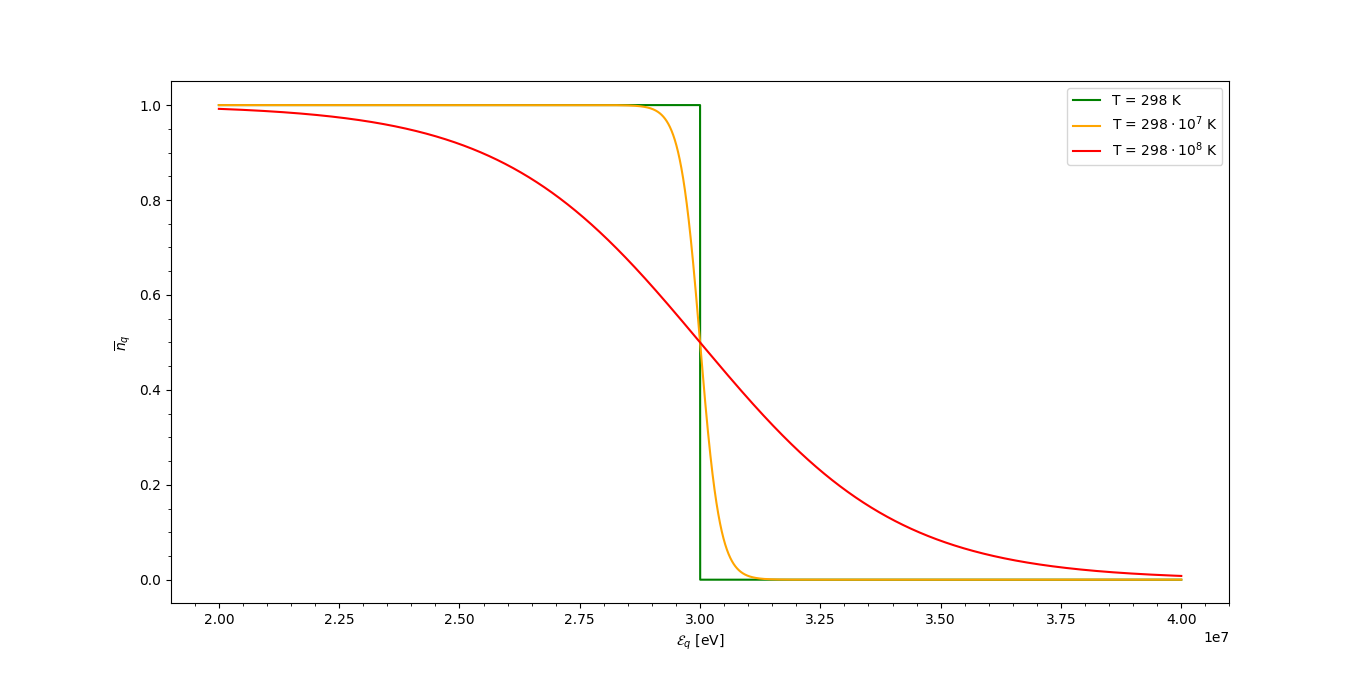
\includegraphics[width=0.9\textwidth]{figures/fermi_dirac.png}
	\caption{\scriptsize Distribuzione di fermi dirac realizzata in python per varie temperature e per $\mu = 30$ MeV, tipico dei gas di elettroni atomici.}
	\label{fig:figures-fermi_dirac-png}
\end{figure}
\noindent
Notiamo come a basse temperature ($kT \ll \mu$) la funzione sia praticamente un gradino che crolla sulla $\mu$, in questo caso lo smusso del gradino è proprio dell'ordine di $kT$.\\
Di fatto a $T\approx 0$ si ha che le particelle si dispongono in modo da minimizzare l'energia (andranno nei livelli energetici più bassi), quindi se voglio aggiungere una particella al sistema dovrò aggiungerla con una energia maggiore di quella delle particelle già presenti perchè tutti gli stati con energia inferiore sono occupati. Quindi per aggiungere questa particella dorvò dare una energia di almento $\mu$. L'energia $\mu = \mathcal{E}_{0}$ a temperatura nulla rappresenta di fatto la linea di demarcazione tra gli stati occupati e gli stati vuoti.\\
Questo ci da informazioni sul fatto che, se $T \to 0$, il potenziale chimico non potrà essere negativo perchè in tal caso il numero di particelle medio per ogni stato è nullo, quindi sparirebbero tutte le particelle dal sistema.\\
Ricordiamo che stiamo sempre considerando il sistema all'equilibrio con un bagno termico in cui abbiamo tenuto $\mu $ costante \footnote{Questo a livello fisico significa poter variare il numero di particelle al variare della temperatura, infatti il potenziale chimico è la variazione dell'energia del sistema rispetto al numero di particelle: per mantenerlo costante al variare dell'energia serve che cambi il numero di particelle.}, variare la temperatura significa variare la temperatura di questo "universo".\\
Spesso nei sistemi veri dobbiamo tener di conto che il numero di particelle del sistema in considerazione (bagno termico escluso) potrebbe essere fissato. In questo caso la legge resta valida però $\mu$ non è più fissato.\\
In questo caso possiamo aspettarci che esista una temperatura oltre il quale torniamo nella approssimazione classica di Boltzmann quindi il potenziale chimico dovrà tornare negativo e molto grande. \\
Possiamo dire anche qualcosa in più sul numero di particelle totali per questa distribuzione:
\[
	N = \sum_{q}^{} \overline{n}_{q} = \int_{0}^{\infty} \rho ( \mathcal{E} ) \cdot \frac{1}{\exp\left( \frac{\mathcal{E} -\mu }{kT} + 1 \right) } d\mathcal{E} 
.\] 
\paragraph{Distribuzione di Bose-Einstein e Bosoni}%
Nel caso in cui le particelle abbiano spin intero non abbiamo più nesuna condizione sulla occupazione degli stati, quindi non possiamo più tagliare al secondo termine nella sommatoria \ref{eq:Landau-Generic}, possiamo invece fare un cambio di variabile:
\begin{align}
	x = \exp\left( \frac{\mu -\mathcal{E} }{kT} \right) \implies
	\Omega _{q} = -kT \ln \left[ \sum_{n_{q}}^{} x^{n_{q}} \right] 
.\end{align}
Sappiamo che per non esplodere questa serie geometrica necessita che $x<1$, quindi che $\mu < \mathcal{E} _{q}$.
L'ultima disuguaglianza deve essere vera per tutti gli $\mathcal{E}_{q}$, quindi nel caso peggiore per lo stato con $\mathcal{E} = 0$, abbiamo allora una condizione sul potenziale chimico per la convergenza della serie:
\[
	\mu < 0
.\] 
Questo ci va bene perchè è conforme con quanto detto per il regime classico, dove anche in quel caso $\mu$ doveva essere negativo (in tal caso c'era una ulteriore condizione: doveva essere molto negativo).\\
Visto che la serie per $\Omega _{q}$ è geometrica si ha che la somma vale:
 \[
	 \Omega _{q} = kT \ln\left( 1-\exp\left( -\frac{\mathcal{E} _{q}-\mu }{kT} \right)  \right) 
.\] 
Quindi ci ricaviamo il numero medio di particelle: 
\[
	\overline{n}_{q} = - \frac{\partial \Omega _{q}}{\partial \mu } = \frac{1}{\exp\left( \frac{\mathcal{E} _{q}- \mu }{kT} \right)-1 }
.\] 
Abbiamo ottenuto una distribuzione simile alla Fermi-Dirac con un segno diverso, quel segno cambia pesantemente la forma della distribuzione che chiameremo:
\begin{defn}[Distribuzione di Bose-Einstein]{def:Distribuzione di Bose-Einstein}
	Il numero medio di particelle negli stati di singola particella $q$ per un gas di bosoni è dato da:
	\[
		\overline{n}_{q} = \frac{1}{\exp\left( \frac{\mathcal{E} _{q}-\mu}{kT} \right) - 1}
	.\]
\end{defn}
Graficamente la distribuzione con $\mu$ fissato è così fatta:
\begin{figure}[H]
	\centering
	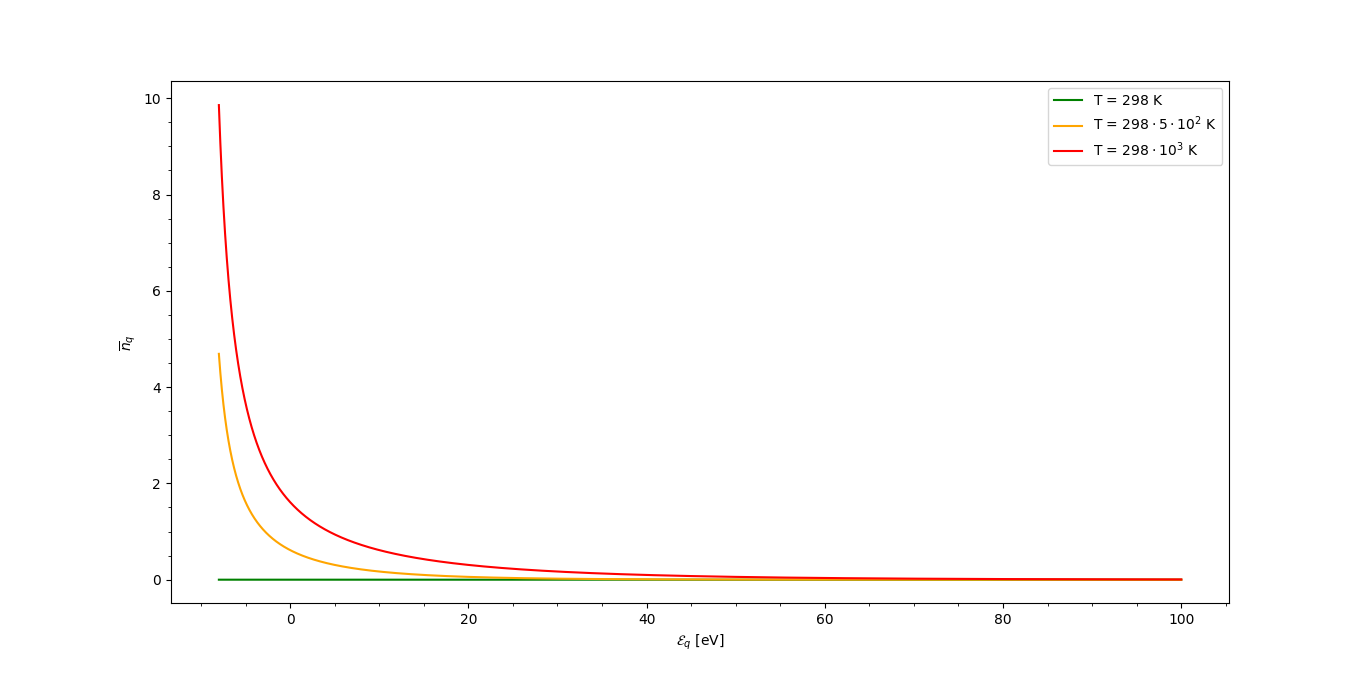
\includegraphics[width=0.95\textwidth]{figures/bose_einstein.png}
	\caption{\scriptsize Distribuzione di Bose-Einstein per $\mu = -10$ eV fissato.}
	\label{fig:figures-bose_einstein-png}
\end{figure}
\noindent
Questa è la Bose Einstein, e le particelle di spin intero sono perciò detti Bosone.\\
Tenere $\mu $ fissato anche in questo caso significa tenere libero il numero di particelle del sistema che quindi potrà essere scambiato con il bagno termico. La conseguenza che ne risulta dal grafico è che al diminuire della temperatura le particelle tenderanno a scappare dal sistema per spalmarsi in tutto l'universo (nei livelli di energia più bassa disponibili).\\
Nel limite classico entrambe le distribuzioni tornano al limite di Boltzmann classico.

\lez{8}{04-03-2020}{}
Abbiamo visto nella scorsa lezione che per un gas di Bosoni che può scambiare particelle con il bagno termico se la temperatura tende a zero allora numero di particelle medie per cella tende a zero: il sistema si svuota.\\
Noi considereremo più spesso casi in cui il numero di particelle è fissato, in tal caso il potenziale chimico diventa una funzione della temperatura.\\
Siccome il numero totale di particelle è dato da:
\[
	\int_{0}^{\mathcal{E} } \rho ( \mathcal{E} ) \overline{n}( \mathcal{E} ) d\mathcal{E} = N 
.\] 
È necessario che il potenziale chimico cresca e tenda quindi a zero cercando di mantenere costante l'integrale sotteso alla curva per energie positive.
\begin{figure}[H]
    %This is a custom LaTeX template!
    \centering
    \incfig{bose-einstein-con-t-tendente-a-zero-e-numero-di-particelle-fissato}
    \caption{\scriptsize Bose-Einstein con T tendente a zero e numero di particelle fissato.}
    \label{fig:bose-einstein-con-t-tendente-a-zero-e-numero-di-particelle-fissato.}
\end{figure}
\noindent
Quindi a $T=0$ abbiamo che l'unico stato occupato è lo stato fondamentale. Prossimamente discuteremo l'andamento di $\mu $ al variare di T, vedremo che $\mu $ diventa effettivamente zero per una temperatura di poco maggiore dello zero assoluto, raggiungendo uno stato della materia in cui il numero di particelle nello stato fondamentale è macroscopico \footnote{detto condensato di Bose-Einstein}.
\subsection{Fluttuazioni quantistiche vs fluttuazioni termodinamiche}%
Nella derivazione delle due distribuzioni abbiamo effettuato con leggerezza il passaggio al continuo, dovremmo almeno verificare che questo passaggio è lecito avendo abbandonato il regime di gas ideale.\\
Se chiamiamo $\delta \mathcal{E} $ la distanza media tra gli stati dobbiamo verificare che:
\[
	\delta \mathcal{E} \ll \sqrt{\overline{\left( \Delta \mathcal{E}  \right) ^2}} 
.\] 
In questo modo le fluttuazioni termodinamiche sono più importanti delle fluttuazioni quantistiche e ci è permesso fare un passaggio al continuo come già argomentato.\\
Le fluttuazioni termodinamiche dell'energia della singola particella sono dell'ordine di $kT$, mentre quelle quantistiche  $\frac{\hbar^2}{2m}\left( \frac{2\pi}{L} \right) ^2$ (nel caso di particelle confinate in una scatola di dimensioni caratteristiche linearri L).\\
Se prendiamo $L \approx 1cm$, $m \sim 10^{-24}g$ otteniamo che per avere $\overline{\left( \Delta \mathcal{E}  \right) ^2}\gg \delta \mathcal{E} $ serve $T> 10^{-10}K$. Per questo motivo in sistemi fisici reali non abbiamo problemi di fluttuazioni quantistiche.\\

\subsection{Spin nel calcolo della $\rho ( \mathcal{E} ) $}%
Quando a partire dagli impulsi siamo passati all'energia nella sezione \ref{subsec:dens-stati} ci siamo dimenticati dello spin che è un'altra variabile delle nostre particelle. Sappiamo che la degenerazione di spin è $2s+1$ \footnote{Dove $s$ è lo spin appunto}. Quindi se chiamiamo la densità di stati senza considerare lo spin $\rho '( \mathcal{E} ) $ si ha che la correzione dovuta allo spin su questa è: 
\[
	\rho ( \mathcal{E} ) = \rho'( \mathcal{E} ) \cdot  \left( 2s + 1 \right)   = g \rho '( \mathcal{E} ) 
.\] 
Visto che noi parliamo di fermioni e bosoni le nostre correzioni sono relativamente 2 e 1, fatta eccezione per i fotoni ed i fononi \footnote{Questi ultimi si occupano delle vibrazioni dei cristalli, sono quanti o quasi-particelle.}.
Infatti nel caso dei fononi abbiamo tre degenerazioni dovute ai gradi di liberta vibrazionali, mentre per i fotoni sappiamo invece che abbiamo due degenerazioni dovute alle possibili polarizzazioni.\\
La densità di stati che continueremo ad usare per qualche lezione è quella ricavata nella sezione citata sopra:
\[
	\rho ( \mathcal{E} ) d\mathcal{E} = \frac{4\pi\sqrt{2} V m_{3 /2}}{\left( 2\pi \hbar \right)^3 } \mathcal{E} ^{1 /2} g d\mathcal{E} 
.\] 
Relativa ad un sistema tridimensionale di particelle con energia $p^2/2m$.

\subsection{Correzione al secondo ordine per l'equazione di stato dei gas ideali}%
Cerchiamo di capire cosa succede quando siamo in condizioni tali da non poter usare l'approssimazione di gas ideali "per poco" quindi quando la disuguaglianza \ref{eq:ideal_gas_approx} non è forte, ma è soltanto una disuguaglianza.\\ 
Per farlo andiamo all'ordine successivo nelle approssimazioni fatte con quella disuguaglianza, che ricordiamo essere:
\[
	\exp\left( \frac{\mu }{kT} \right) \ll 1
.\] 
Quindi vediamo come si modifica l'equazione di stato dei gas ideali quando iniziamo a tener di conto degli effetti quantistici.\\
Il potenziale di Landau nei due casi studiati sopra è:
\[
	\Omega^{\text{FD}}_{\text{BE}} = \mp kT \sum_{q}^{} \ln\left[ 1 \pm \exp\left( - \frac{\mathcal{E} _{q}-\mu }{kT} \right)  \right] 
.\] 
Dove il segno superiore è per la Fermi-Dirac, il segno inferiore è per la Bose-Einstein.\\
Per arrivare alla approssimazione classica nella abbiamo tenuto soltanto i termini al primo ordine in $x$, adesso usando l'espressione di $\Omega$ per bosoni e fermioni possiamo anche andare al secondo ordine $x^2$:
\[
	\Omega = -kT \sum_{q}^{} \exp\left( - \frac{\mathcal{E} _{q}-\mu }{kT} \right) \pm \frac{kT}{2}\sum_{q}^{} \exp\left[ - \frac{2 \left( \mathcal{E} _{q}-\mu  \right) }{kT} \right] 
.\]
Mentre la prima parte è il potenziale di Landau già trovato in ambito classico il secondo pezzo inizia a differenziarsi nel caso si tratti di fermioni o bosoni:
\[
	\Omega = \Omega _{\text{class}} \pm \frac{kT}{2}\sum_{q}^{} \exp\left[ - \frac{2 \left( \mathcal{E} _{q}-\mu  \right) }{kT} \right] 
.\]
Possiamo fare il conto della correzione passando al continuo visto la valutazione sulle fluttuazioni fatta due sezioni sopra:
\[
	\sum_{q}^{} \exp\left( -\frac{2\mathcal{E} _{q}}{kT} \right) = \int_{0}^{\infty}  \rho ( \mathcal{E} ) \exp\left( - \frac{2\mathcal{E} }{kT} \right) d\mathcal{E} =
	\left( \frac{1}{2} \right) ^{3 /2}\int_{0}^{\infty} \rho ( \overline{\epsilon }) \exp\left( - \frac{\overline{\epsilon }}{kT} \right) d \overline{\epsilon } 
.\] 
Dove abbiamo fatto il cambio di variabile $\overline{\epsilon }= 2\mathcal{E} $, abbiamo inoltre considerato il fatto che in $\rho ( \mathcal{E} ) \propto \mathcal{E} ^{1 /2}$ quindi esce quel fattore alla $3 /2$ dall'integrale.
Quindi la correzione alla $\Omega _{\text{class}}$ è la seguente:
\[
	\pm kT \left( \frac{1}{2} \right) ^{5 /2} \exp\left( \frac{\mu }{kT} \right) \int_{0}^{\infty} \rho ( \overline{\epsilon }) \exp\left( - \frac{\overline{\epsilon }}{kT} \right) d \overline{\epsilon } 
.\] 
Notiamo adesso che la maggior parte della correzione che abbiamo ottenuto non è altro che $\Omega _{\text{class}}$ stessa, possiamo allora compattare l'espressione raggruppando questa quantità (ponendo attenzione ai segni):
\[
	\Omega = \Omega _{\text{class}} \left[ 1 \mp \frac{\exp\left( \frac{\mu }{kT} \right) }{2^{5 /2}} \right] 
.\] 
Siamo pronti a ricavare l'equazione del gas perfetto con effetti quantistici:
\[
	\Omega  = - PV
.\]  
\[
	\Omega _{\text{class}} = -NkT
.\]
allora avviamo la correzione
\[
	PV = NkT\left[ 1 \mp \frac{\exp\left( \frac{\mu }{kT} \right) }{2^{5 /2}} \right] \label{eq:eq-id-corretta_1}
.\] 
Possiamo chiederci se questa correzione ha senso, alla luce del fatto che la correzione per i fermioni è negativa e che per questi non possiamo avere più di una particella per stato. Una forma equivalente è la seguente:
\[
	P = \frac{N}{V} kT \left[ 1 -+ \frac{\exp\left( \frac{\mu }{kT} \right) }{2^{ 5 /2}} \right] 
.\] 
Quindi per un gas di fermioni alla temperatura T con densità $N /V$ la pressione è inferiore a quella di un gas classico, mentre per un gas di bosoni la pressione la pressione è inferiore. \\
Questo è assolutamente contro intuitivo: i fermioni (che hanno al massimo una particella per stato) ci aspettiamo abbiano una "repulsione intrinseca" maggiore dei bosoni che non hanno problemi ad ammassarsi negli stati a bassa energia. Di conseguenza ci si aspetta anche che per i fermioni la pressione sia maggiore che per i gas ideali e viceversa per i bosoni. \\
Il segno del secondo termine nella \ref{eq:eq-id-corretta_1} dovrebbe essere allora invertito per soddisfare il nostro intuito. Tuttavia la derivazione che abbiamo seguito sembra corretta, non ci sono evidenze di errori algebrici. Deve esserci qualcosa di concettualmente sbagliato quindi.\\
Possiamo provare con un'altra derivazione passando questa volta dalla energia libera F, ricordiamo la proprietà che lega le variazioni dei potenziali termodinamici durante una trasformazione sul sistema:
\[
	\left.\delta F\right|_{T,V,N} = \left.\delta \Omega \right|_{T,V,\mu }
.\]
La variazione che consideriamo è la correzione da sistema classico a sistema "leggermente quantistico" come spiegato all'inizio.
Possiamo scrivere che:
\[
	\Omega ( T,V,\mu )  = \Omega _{\text{class}} + \delta \left.\Omega \right|_{T,V,\mu }
.\] 
Con $\left.\delta \Omega \right|_{T,V, \mu}$ che è quella calcolata prima. Avremo di conseguenza per la F:
\[
	F( T,V,N) = F_{\text{class}} + \left.\delta F\right|_{T,V,N}
.\] 
Quindi la correzione trovata per il potenziale di Landau sarà la stessa di quella per l'energia libera, l'unica accortezza da tenere è che nel primo caso era fissato il potenziale chimco, nel secondo il numero di particelle. Vedremo che la chiave del "mistero" sopra sarà esattamente questa.\\
Abbiamo trovato che:
\[
	\delta \Omega = \mp \Omega _{\text{class}}\frac{\exp\left( \mu  \right)kT }{2^{5 / 2}} = \pm NkT \frac{\exp\left( \frac{\mu }{kT} \right) }{2 ^{5 /2}}
.\] 
Quello che vorremmo fare adesso è eliminare la dipendenza esplicita da $\mu $ di questa correzione per poterla sostituire in F in funzione delle sue variabili predilette, per farlo ricordiamo l'equazione \ref{eq:mu_classico} del caso classico:
\[
	\mu _{\text{class}} = -kT \ln\left( \frac{V}{N\Lambda ^3} \right) 
.\] 
Per toglierci di mezzzo $\mu $ basterà sostituirlo in $\delta \Omega $, infatti la correzione su $\mu _{\text{class}}$ inserita all'interno della variazione sul potenziale di Landau genera una correzione all'ordine successivo che possiamo trascurare. Dalla sostituzione si ricava che:
\[
	F = F_{\text{class}} \pm \frac{N^2kT\Lambda ^3}{2^{5 /2}V}
.\] 
Quindi ricaviamo la legge di stato:
\[
	P = - \frac{\partial F}{\partial V} = P_{\text{class}} \pm \frac{N^2kT\Lambda ^3}{2^{5 /2}V^2} = \frac{NkT}{V}\left( 1 \pm \frac{N\Lambda ^3}{2^{5 /2}V} \right) 
.\] 
Abbiamo ottenuto i segni che intuitivamente ci si aspetterebbe, resta tuttavia il problema che i due metodi hanno prodotto risultati all'apparenza contrastanti.\\
Nel primo caso abbiamo trovato la pressione da $\Omega $, nel secondo partendo da $F$. Ragionando con la $\Omega $ il numero di particelle non è costante durante una compressione. Questo ci porta in errore quando facciamo ragionamenti di intuito come abbiamo fatto sopra. Il modo giusto (nel quale ha senso applicare il nostro ragionamento) è quello di partire dalla $F$. Infatti quello che ci aspettiamo fisicamente è che, durante una compressione, il numero di particelle resti invariato.\\
Resta il fatto che non abbiamo trovato l'inghippo matematico alla base del problema, infatti quello che abbiamo fatto nel secondo caso è prendere la correzione calcolata con $\Omega $ ed inserirla nell'espressione per $F$, quindi l'errore avrebbe dovuto comparire anche alla fine del secondo ragionamento.\\ 
Dobbiamo stare attenti al fatto che nel primo caso $N = N ( \mu ) $ ed in particolare si ha che, fissato un $\mu $:
\[
N = N_{\text{class}}( \mu ) \neq N_{2^o\text{ordine}}( \mu ) 
\]
Abbiamo quindi un abuso di notazione, il numero di particelle $N$ che consideriamo per il nostro sistema non è più quello classico ma è anch'esso corretto al secondo ordine.\\
Quindi quando facciamo la differenza rispetto alla funzione classica e cerchiamo di capire se ci tornano le considerazioni su fermioni e bosoni sbagliamo nel fatto il numero di particelle non è lo stesso rispetto al caso classico.\\
Non possiamo dire lo stesso del secondo caso, infatti il numero di particelle in  $F$ è fissato, il chè non ci porta in errore quando sostituiamo l'equazione dei gas perfetti per eliminare $P_{\text{class}}$.

\subsection{Gas di Fermioni: elettroni di conduzione in un metallo}%
Riprendiamo la distribuzione di Fermi-Dirac per trattare un gas di elettroni in un metallo.\\
La prima cosa da fare è calcolare il numero di particelle $N$ :
\[
	N = \int_{0}^{\infty} \frac{\rho ( \mathcal{E} ) d\mathcal{E} }{\exp\left( \frac{\mathcal{E} -\mu }{kT}+1 \right) }
.\] 
Normalmente questo sarebbe integrato da $0$ ad $\infty$, nel limite di $T \to 0$ si può approssimare la distribuzione da un gradino unitario, quindi:
\[
	N \to \int_{0}^{\mathcal{E} _{F}}  \rho ( \mathcal{E} ) d\mathcal{E}  
.\] 
Quindi possiamo, anzichè integrare la $\rho ( \mathcal{E} ) $ brutta, possiamo prendere il volume della sfera nello spazio delle fasi di raggio $p _{F}$ tale che $\mathcal{E} _{F} = p_{F}^2 /2m$, moltiplicarlo per il volume in questione $V$, dividere per il volume della cella unitaria (senza scordarsi dello spin).
\[
	N = \frac{g V \left( \frac{4}{3} \pi p_{F}^3 \right) }{\left( 2\hbar \pi \right) ^3} 
.\] 
Possiamo ricavare $p_{F}$ da quest'ultima oppure direttamente $\mathcal{E} _{F}$ dall'integrale, quello che si ottiene è sempre:
\[
	\mu _{0} = \mu ( 0) = \mathcal{E} _{F} = \frac{\left( 2\pi \hbar  \right) ^2}{2m} \left( \frac{N}{V} \right) ^{2 /3} \left( \frac{3}{4\pi q} \right) ^{2 /3}
.\]
Possiamo trovare l'energia media a $T\to 0$:
\[
	\overline{\mathcal{E} } = \frac{\int_{0}^{\mathcal{E} _{F}} \mathcal{E} \rho ( \mathcal{E} ) d\mathcal{E} }{\int_{0}^{\mathcal{E} _{F}} \rho ( \mathcal{E} ) d\mathcal{E}  }=
	\frac{\int_{0}^{\mathcal{E} _{F}} \mathcal{E} ^{3 /2}d\mathcal{E}  }{\int_{0}^{\mathcal{E} _{F}} \mathcal{E} ^{ 1/ 2}d \mathcal{E}  } = 
	\frac{3}{5} \mathcal{E} _{F}	
.\] 
Di conseguenza l'energia totale sarà:
\[
	E( T=0)  = N \overline{\mathcal{E} } = \frac{3}{5} \mathcal{E}_{F} N
.\] 
Mentre la pressione è data da:
\[
	P = - \left.\frac{\partial E}{\partial V} \right|_{N} = \frac{2}{3}\frac{E}{V}
.\] 
Quest'ultima l'avevamo già ricavata a partire dal fatto che la legge di dispersione dell'energia è $p^2/2m$, senza nessuna assunzione. Notiamo che la pressione a $T = 0$ non va a zero. Questo non succede per il gas classico.\\
Vediamo invece come cambiano le cose se la temperatura non è nulla ma vale 
\[
T \ll T_{F} 
\]
Dove $T_{F}$ è la temperatura definita a partire da $kT_{F} = \mathcal{E} _{F}$, ed è detta temperatura di Fermi. Visto che abbiamo espresso $\mathcal{E} _{F}$ possiamo esprimere anche $T_{F}$
\[
	T_{F} = \frac{\left( 2\pi \hbar  \right)^2}{2m k} \left( \frac{3}{4\pi q} \right)^{2 /3} \left( \frac{N}{V} \right) ^{2 /3}
.\] 
Per $T\ll T_{F}$ si ha che la distribuzione di Fermi è molto simile al gradino, questo ci permetterà di fare delle approssimazioni. Vediamo adesso con un esempio pratico se in condizioni normali tale disuguaglianza è rispettata.\\
Visto che conosciamo la densità di elettroni liberi in un metallo possiamo calcolare la $T_{F}$ di quest'ultimo. Nel rame abbiamo ad esempio $\rho _{e}= 8.5 \cdot 10^{22}$ e/cm$^3$, messa nella formula per la temperatura di Fermi ci restituisce:
\[
	T_{F, \text{rame}} = 8.5 \cdot 10^{4} K
.\] 
Se ne conclude che a temperatura ambiente siamo sempre nel regime $T \ll T_{F}$.\\
Tipicamente la $T_{F}$ è maggiore della temperatura di fusione dei metalli. Questo ci dice che gli elettroni nei metalli sono essenzialmete quantistici, abbiamo una distribuzione di questi nei livelli completamente diversa da quella prevista da Boltzmann.
\begin{defn}[Gas Degenere]{def:Gas Degenere}
	Un gas si dice degenere quando si trova in un regime in cui non vale più l'approssimazione di gas ideale, tale gas sarà quindi descritto da una distribuzione non classica come la Fermi-Dirac oppure la Bose-Einstein.\\
	Sono ad esempio degeneri gli elettroni di un metallo.
\end{defn}
Abbiamo tuttavia delle precisazioni da fare, poichè gli elettroni in un metallo non solo fanno cadere l'approssimazione di gas ideale ma potrebbero uscire anche dalla approssimazione di gas perfetto!\\
Infatti stiamo operando in situazioni in cui questi sono degeneri (quindi il più compatti possibile nei limiti imposti dalla Fermi-Dirac), la loro vicinanza ci induce a pensare che non si possa più trascurare l'interazione coluombiana. Inoltre sono all'interno di un metallo che idealmente sta perdendo elettroni in continuazione, quindi saranno immersi in una miriade di ioni che sono un'altra possibile fonte di interazione.\\
Fortunatamente la situazione si risolve assumendo che gli elettroni abbiano lunghezze d'onda grandi rispetto alla distanza tra gli atomi del solido.\\
In questo modo gli elettroni è come se vedessero un background di carica uniforme proveniente da tutti gli ioni, questo può essere il fondo della buca di potenziale dato dalla scatola \footnote{In questo ragionamento il "confinamento" dovuto alle pareti della scatola ed il background di ioni sono la stessa cosa!}. Inoltre il fondo positivo scherma l'interazione culoumbiana tra gli elettroni, quindi in questa ottica possiamo tenerci gli elettroni come gas perfetto.\\
Ci aspettiamo inoltre che gli elettroni possano comunque scatterare o interagire per collisioni, tuttavia se $T \ll T_{F}$ questi fermioni non avranno comunque livelli liberi per cambiare la loro energia qualunque tipo di interazione facciano. \\
Possiamo anticipare che i fenomeni di scattering coincolgeranno solo gli elettroni aventi energie prossime all'energia di fermi perchè sono gli unici ad avere un pò di stati vuoti nelle vicinanze per potersi spostare.\\
Essenzialmente, quando faremo il modello di gas di elettroni nei solidi, potremo trattare tutto come un gas perfetto, l'unica cosa che cambia è che la massa nella relazione:
\[
	\mathcal{E} = \sum_{}^{} \frac{P^2}{2m}
.\] 
Non sarà la massa dell'elettrone libero, sarà una massa efficace che tiene conto del fatto che gli elettroni non si muovono in uno spazio vuoto ma sono "vincolati" in uno spazio occupato da altri elettroni e nuclei.\\
Storicamente il fatto che all'interno dei metalli vi fossero elettroni liberi fu accolto in modo positivo dalla comunità scentifica che iniziò subito ad attrezzarsi per misurare e verificare questo fatto.\\ 
I fisici tirarono fuori una densità media di elettroni all'interno del metallo facendo delle misure, furono quindi in grado di tirare fuori un calore specifico sperimentale. Essi si aspettavano che il calore specifico per questo gas di particelle libere nel metallo fosse quello classico: 
\[
	C_{V}= \frac{3}{2}Nk
.\] 
Quest'ultima risultò incompatubile con le misure. Il calore specifico ottenuto era molto inferiore di quello atteso. Noi sappiamo che il motivo proviene dal fatto che la statistica non è più quella di Boltzmann. \\
Se ad esempio consideriamo la statistica di Fermi-Dirac per $T \approx 0$ ed aumentiamo di poco la temperatura si ha che gli unici elettroni che cambiano energia sono quelli che stanno in un intorno largo $kT$ dell'energia di fermi, per tutti gli altri non cambia assolutamente nulla.\\ 
Ci aspettiamoche il numero totale di elettroni che contribuiscono al calore specifico non sia $N$ ma sia solo una frazione:
\[
	N_{C_{V}} \sim N\cdot \frac{T}{T_{F}}
.\] 
Il guadagno di energia di questi elettroni per fare un salto di energia sarà:
\[
	\Delta E = \frac{N kT^2}{T_{F}}
.\] 
Quindi per definizione di calore specifico si ha che:
\[
	C_{V} \approx \frac{\Delta E}{\Delta  T} = \alpha \frac{T}{T_{F}} 
.\] 
In effetti si riscontra che il calore specifico nei metalli ha proprio questo andamento lineare nella temperatura.\\
Cerchiamo di sviluppare le proprietà termiche del gas di elettroni, le useremo per esempio per descrivere il calore specifico. Non faremo più gli integrali in modo da approssimare la Fermi-Dirac come funzione a gradino ma ci teniamo l'espressione con la dipendenza dalla temperatura.
\[
	\Omega = -\frac{2}{3} \frac{4\pi V g \sqrt{2}  m ^{3 /2}  }{\left( 2\pi\hbar  \right) ^3} \int_{0}^{\infty} \frac{\mathcal{E} ^{3 /2}d\mathcal{E} }{\exp\left( \frac{\mathcal{E} -\mu }{kT} \right) +1 } 
.\] 
Siamo comunque nelle ipotesi in cui $T\ll T_{F}$, quindi cercheremo di riscrivere l'integrale di sopra con una correzione all'ordine opportuno in questo modo:
\[
	I = \int_{0}^{\infty} \frac{f( \mathcal{E} ) }{\exp\left( \frac{\mathcal{E} -\mu }{kT} \right) +1 }d\mathcal{E}  = I_0 + \delta  I 
.\] 
Dove il termine $I_0$ introdotto è:
\[
	I_0 = \int_{0}^{\mathcal{E} _{F}} f( \mathcal{E} ) d\mathcal{E} 
.\] 
Cercheremo di fare una espansione di $I$ in funzione della temperatura:
\[
	I = I_0 + \left.\frac{\partial I}{\partial T} \right|_{T =0} + \frac{1}{2}\left.\frac{\partial ^2I}{\partial T^2} \right|_{T = 0} T^2 + \ldots
.\] 
Prima di procedere dobbiamo chiederci se ci basta una correzione al primo ordine o se dobbiamo correggere con ordini successivi. Questo possiamo capirlo dalla forma della distribuzione nell'intorno della energia di fermi:
\begin{figure}[H]
    %This is a custom LaTeX template!
    \centering
    \incfig{correzione-per-il-potenziale-di-landau-nella-statistica-di-fermi-dirac}
    \caption{\scriptsize Correzione per il potenziale di Landau nella statistica di Fermi-Dirac, in tratteggiato la curva con $T=0$, in continuo la linea con $T\ll T_{F}$}
    \label{fig:correzione-per-il-potenziale-di-landau-nella-statistica-di-fermi-dirac}
\end{figure}
\noindent
La variazione sull'area $I$ cercata sarà la differenza tra la curva tratteggata e la curva continua, possiamo vedere intuitivamente come al primo ordine questa differenza debba annullarsi per simmetria. Per questo la correzione al primo ordine si annulla, quindi al primo ordine $N$ resta costante.\\ 
Per calcolare le correzioni al secondo ordine facciamo un cambio di variabile: passiamo da $\mathcal{E} $ a $z = \exp\left( \frac{\mathcal{E} -\mu }{kT} \right) $ ed introduciamo due funzioni: 
 \begin{align*}
	&g_1( z)  = \begin{cases}
		0 \quad z <0\\
		\frac{1}{e^{z}+1} \quad z > 0
	\end{cases}\\
	&g_0( z) =
 \begin{cases}
		\frac{1}{e^{-z}+1} \quad z < 0 \\
		0 \quad z >0
	\end{cases}
.\end{align*}
Vediamo che queste non sono altro che le due "fette" che differiscono tra la distribuzione a temperatura nulla e quella a temperatura molto bassa, soltanto che la $g_0$ è la parte in alto ribaltata:
\begin{figure}[H]
    %This is a custom LaTeX template!
    \centering
    \incfig{g1-e-g0}
    \caption{\scriptsize Plot delle due funzioni scritte sopra.}
    \label{fig:g1-e-g0}
\end{figure}
La differenza dell'integrale della fermi dirac tra $T=0$ e  $T\ll T_{F}$ sarà dato da:
\[
	\delta I = \int_{-\infty}^{\infty} f( \mathcal{E} ) \left[ g_1( z) - g_0( z)  \right] d\mathcal{E}   = \int_{-\infty}^{\infty}  f ( \mu + kTz) 
	\left[ g_1( z) - g_0( 0)  \right] kT dz
.\] 
L'estremo inferiore di integrazione sarebbe dato dal fatto che $\mathcal{E} _{\text{min}}=0 \implies z_{\text{min}}= - \mu /kT$, tuttavia possiamo anche mandarlo a $-\infty$ poichè per il valore di $z_{\text{min}}$ la differenza tra le $g_{i}$ è praticamente ormai nulla, quindi andare a $-\infty$ non compromette il risultato della somma.\\
Procediamo al calcolo dell'ultimo integrale, dal momento che l'integrale è pesato solo attorno al potenziale chimico possiamo sviluppare $f( \mu + kTz) $ attorno a $0$:
\[
	f( \mu + kTz) = f( \mu )  + kTz \left.\frac{\partial f}{\partial \mathcal{E}  } \right|_{\mathcal{E} =\mu } + \ldots= f( \mu )+ kTzf'( z)  
.\] 
Sostituendo troviamo:
\[
	\delta I = kTf( \mu )  \int_{-\infty}^{\infty} \left[ g_1( z)- g_0( z)   \right] dz + ( kT) ^2f'( z) \int_{-\infty}^{\infty} z \left[ g_1( z) -g_0( z)  \right] dz  
.\] 
Quindi aver fatto lo sviluppo attorno al potenziale chimico della $f$ è stato equivalente a fare lo sviluppo agli ordini successivi della temperatura di $\delta I$.\\
Il primo pezzo (che è il primo ordine) è esattamente zero perchè le due aree delle $g_{i}$ si elidono in questi estremi di integrazione per simmetria. Il secondo pezzo avendo z nell'integrale "rompe la simmetria" delle $g$ permettendo così che si sommino i contributi di queste due.

\lez{9}{09-03-2020}{}
Procediamo al calcolo del secondo integrale nella precedente, abbiamo le espressioni per le funzioni $g_{i}$ dalle \ref{eq:g_1} e \ref{eq:g_0} :
\[
	\int_{0}^{\infty} zg_1 dz - \int_{-\infty}^{0} zg_0 dz = + 2\int_{0}^{\infty} \frac{z}{e^{z}+1} dz = \frac{\pi^2}{6}
.\] 
Questo integrale ci permette di trovare la correzione alla tipologia di integrali che volevamo risolvere nella lezione precedente (che avevamo nominato $I$):
\[
	I = \int_{0}^{\mu } f( \mathcal{E} ) d\mathcal{E} + \frac{\pi^2}{6}f'( \mu ) \left( kT \right) ^2 
.\] 
Di questo tipo era il potenziale di Landau della \ref{eq:landau-lez-8}, sostituendo in quella equazione:
\[
	\Omega = - \frac{2}{3}\frac{4\pi V g \sqrt{2} m ^{3 /2}}{\left( 2\pi \hbar \right)^3 }
	\left[ \frac{2}{5}\mu ^{5 /2} + \frac{\pi^2}{4}\mu ^{1 /2} \left( kT \right) ^2 \right] 
.\] 
Grazie a questo risultato si trova anche il numero di particelle in funzione della temperatura:
\[
	N = - \frac{\partial \Omega }{\partial \mu }  = - \frac{2}{3}\frac{4\pi V g \sqrt{2} m ^{3 /2} }{\left( 2\pi \hbar \right)^3 }
	\left[ \mu ^{3 /2}+ \frac{\pi^2}{8} \frac{\left( kT \right)^2}{\mu ^{1 /2}} \right] 
.\] 
Possiamo scriverlo un funzione del numero di particelle a $T = 0$:
\[
	N_0 = - \frac{2}{3}\frac{4\pi V g \sqrt{2} m ^{3 /2}\mu ^{3 /2}}{\left( 2\pi \hbar \right)^3 }
.\] 
In questo modo si ottiene una forma più compatta del numero di particelle:
\[
	N = N_0 \left[ 1 + \frac{\pi^2}{8}\left( \frac{kT}{\mu } \right) ^2 \right] 
.\] 
Questo è il caso in cui gli elettroni sono liberi di lasciare il metallo, in realtà succede più spesso che il numero di particelle resti costante nel caso di elettroni liberi in un metallo. Quindi al variare della temperatura dovrà variare il potenziale chimico.\\
In realtà l'espressione trovata è sufficiente per trovare il potenziale chimico: chiamiamo $\mu_0$ il potenziale chimico a $T = 0$, si ha che
\[
	N_0 = \left.N\right|_{T=0, \mu_0}
.\] 
Se cambiamo la temperatura avremo la seguente espressione per il numero di particelle:
\[
	N( T, \mu_0)  = N_0\left[ 1 + \frac{\pi^2}{8}\left( \frac{kT}{\mu_0} \right)^2  \right] 
.\]
Potremmo fare la stessa cosa con un $\mu $ diverso ottenendo (ricordiamo che $N_0$ dipende da $\mu_0^{3 /2}$ ):
\[
	N( T = 0, \mu )  = N( T=0, \mu_0) \left( \frac{\mu}{\mu_0} \right) ^{3 /2} = N_0\cdot \left( \frac{\mu}{\mu_0} \right) ^{3 /2}
.\] 
Di conseguenza abbiamo:
\[
	N( T,\mu ) = N_0\cdot \left( \frac{\mu }{\mu_0} \right)^{3 /2} \left[ 1 + \frac{\pi^2}{8}\left( \frac{kT}{\mu } \right) ^2 \right] 
.\] 
Se eguagliamo $N( T, \mu ) = N( T=0, \mu_0) = N_0 $ troveremo il nostro $\mu $ rispetto a $\mu_0$ che mantiene il numero di particelle costanti:
\[
	N_0 = N_0\left[ 1 + \frac{\pi^2}{8}\left( \frac{kT}{\mu } \right) ^2 \right] \left( \frac{\mu }{\mu_0} \right) ^{3 /2}
.\] 
Possiamo ora fare l'approssimazione 
\[
\left( \frac{kT}{\mu } \right)  \to \left( \frac{kT}{\mu_0} \right) 
\]
Poichè l'errore introdotto facendo questo va all'ordine successivo nella temperatura. Si ottiene:
\[
	\mu = \mu_0\left[ 1- \frac{\pi^2}{12}\left( \frac{kT}{\mu_0} \right)^2 \right] 
.\] 
Questo vale per temperature $T \ll T_{F}$.\\
Quindi abbiamo trovato la correzione per $\mu $, è come ci aspettavamo: la correzione deve essere negativa per mantenere $N$ costante. \\
In realtà questa vale per il gas perfetto di elettroni liberi, in particolare dipende da come è fatta la densità di stati all'interno del sistema (che abbiamo infatti usato).\\
In particolare il potenziale chimico diminuisce all'aumentare dell'energia perchè la densità di stati è una funzione crescente dell'energia, vedremo che non è vero per tutti sistemi. Questo spiegherà perchè in alcuni cristalli il potenziale chimico aumenta con la temperatura.\\
Possiamo adesso trovare l'entropia del gas di fermioni:
\[
	S = - \left.\frac{\partial \Omega }{\partial T} \right|_{V,\mu } = 
		\frac{4\pi V g \sqrt{2} m ^{3 /2}}{h^3} \frac{\pi^2}{3}\mu ^{1 /2} k^2 T
.\] 
Questa in realtà è $S( T, V , \mu ) $ mentre noi vorremmo $S( T,V,N) $ ma se teniamo $N$ costante allora il cambiamento nell'entropia in $\mu $ sarebbe dell'ordine di $T^3$, visto che l'entropia ha andamento in $T$ senza effettuare il conto possiamo concludere che:
\[
	S = \frac{\pi^2}{2}Nk \frac{T}{T_{F}}
.\] 
Mentre per trovare $C_{V}$ basta fare:
\[
	C_{V} = T \left.\frac{\partial S}{\partial T} \right|_{V} = \frac{\pi^2}{2} Nk \frac{T}{T_{F}}
.\] 
Di conseguenza troviamo essenzialmete lo stesso trovato con un ragionamento molto qualitativo nella \ref{eq:stima-Cv-9}, possiamo vederla come verifica di quanto fatto.\\
Quanto visto fin'ora trova buon riscontro nei dati sperimentali, l'unica cosa che non "matcha" benissimo è che nella espressione della temperatura di fermi non avremo più la massa dell'elettrone libero ma avremo una massa efficace dovuta al fatto  che la legge di dispersione dell'elettrone non sarà più quella dell'elettrone libero ma subirà delle sensibili modifiche. \\
La massa efficace è una quantità che può essere misurata anche in modo indipendente: si può sfruttare l'effetto Hall (misura della risonanza di ciclotrone). Si applica un campo magnetico costante al metallo del quale vogliamo conoscere la massa efficace degli elettroni, sappiamo che se applichiamo uno di questi campi gli elettroni orbitano nel piano perpendicolare alla direzione di $B$ con una frequenza angolare:
\[
	\omega_{c}= \frac{eH}{ m ^{*}c}
.\] 
Successivamente con la spettroscopia possiamo misurare la distanza tra i livelli energetici e tiriamo fuori il valore della massa da questi.

\subsection{Gas di elettroni con campo magnetico}%
Vediamo cosa avviene al gas di elettroni con l'aggiunta di un campo magnetico $B$. Siamo nelle ipotesi in cui il campo magnetico influenzi soltanto lo spin (al momento), abbiamo già visto un esempio con la magnetizzazione diamagnetica. \\
In questo caso stiamo parlando di Fermioni con spin $1 /2$, quindi avremo due livelli possibili (up e down) con energie $\pm \mu_{m} B$ \footnote{Chiamiamo $\mu _{m}$ il momento magnetico per non confonderci con $\mu $ che è il potenziale chimico.}. L'energia della particella sarà data allora da:
\[
	E_{\uparrow \downarrow} = \frac{p^2}{2m} \pm \mu_{m}B
.\] 
Possiamo allora distinguere due popolazioni di particelle aventi diversa energia. Visto che si tratta di elettroni in un metallo dovremmo usare la statistica di Fermi-Dirac. \\
Le due popolazioni andranno a distribuirsi popolando il livelli energetici partendo da $\pm \mu_{m}B$ fino ad arrivare a $\mu$ come in figura:
\begin{figure}[H]
    %This is a custom LaTeX template!
    \centering
    \incfig{spin-up-per-gas-di-elettroni-nel-campo-magnetico}
    \caption{\scriptsize Posizione dei livelli energetici per le due popolazioni di elettroni.}
    \label{fig:spin-up-per-gas-di-elettroni-nel-campo-magnetico}
\end{figure}
\noindent
Possiamo quindi trattare il gas di elettroni come due gas di particelle diverse aventi il medesimo potenziale chimico.\\
Mettiamoci adesso nel caso in cui la distribuzione di Fermi-Dirac può essere trattata come gradino ($T = 0$) ed indichiamo $g\uparrow$, $g\downarrow$ come la densità di stati dei due gas. Possiamo graficare l'energia al variare di questa densità di stati, nel caso $B = 0$ si ha \footnote{Abbiamo visto questo caso nelle lezioni precedenti, in questo caso $g( \mathcal{E} ) = \rho ( \mathcal{E} ) \propto \sqrt{\mathcal{E} } $}:
\begin{figure}[H]
    %This is a custom LaTeX template!
    \centering
    \incfig{energia-degli-elettroni-senza-campo-b-in-funzione-della-densita-di-stati}
    \caption{\scriptsize Energia degli elettroni senza campo B in funzione della densità di stati}
    \label{fig:energia-degli-elettroni-senza-campo-b-in-funzione-della-densita-di-stati}
\end{figure}
Applicando il campo magnetico questo grafico si modifica in questo modo:
\begin{figure}[H]
    %This is a custom LaTeX template!
    \centering
    \incfig{energia-degli-elettroni-con-campo-b-in-funzione-della-densita-di-stati}
    \caption{\scriptsize Energia degli elettroni con campo B in funzione della densità di stati}
    \label{fig:energia-degli-elettroni-con-campo-b-in-funzione-della-densita-di-stati}
\end{figure}
\noindent
L'integrale della curva in figura ci da il numero di particelle in ciascuna delle due popolazioni ($N_{\uparrow}$, $N_{\downarrow}$) perchè abbiamo assunto che la Fermi-Dirac fosse il gradino unitario.\\
Se invece vogliamo la magnetizzazione avremo:
\[
	M = \left( N_{\uparrow}-N_{\downarrow} \right)\mu_{B}
.\] 
Procediamo quindi al calcolo dell'integrale, per farlo è più facile sciftare le aree in Figura \ref{fig:energia-degli-elettroni-con-campo-b-in-funzione-della-densita-di-stati} nel seguente modo:
\begin{figure}[H]
    %This is a custom LaTeX template!
    \centering
    \incfig{calcolo-del-numero-di-particelle-negli-stati-up-e-down-sciftando-le-aree}
    \caption{\scriptsize Calcolo del numero di particelle negli stati Up e Down sciftando le aree}
    \label{fig:calcolo-del-numero-di-particelle-negli-stati-up-e-down-sciftando-le-aree}
\end{figure}
\noindent
Tipicamente l'energia di fermi è molto grande rispetto a $\mu_{m}B$, questo ci permette di approssimare l'area grigia in Figura \ref{fig:calcolo-del-numero-di-particelle-negli-stati-up-e-down-sciftando-le-aree} con un rettangolo. Inoltre possiamo considerare la $g( \mathcal{E} ) $ costante in tale area \footnote{Si considera adesso la $g( \mathcal{E} ) $ per i singoli spin.} (sempre grazie alla approssimazione di cui sopra), quindi il valore di tale area sarà:
\[
	N_{\uparrow}- N_{\downarrow} = 2\mu _{m}B \cdot g( E_{F}) 
.\] 
Sapendo il valore di $g( E_{F})$ dalla \ref{eq:densita-stati-con-E-fermi} possiamo riscrivere il $\Delta N$ come:
\[
	\Delta N = \frac{3N}{2}\frac{\mu _{m}B}{E_{F}}
.\] 
Abbiamo quindi la magnetizzazione $M = \mu_{m}\Delta N$ e la suscettività 
\[
	\chi = \frac{M}{B} = \frac{3}{2}N \frac{\mu_{m}^2}{E_{F}} \label{eq:suscettivita-pauli}
.\] 
L'equazione \ref{eq:suscettivita-pauli} è detta Espressione classica del paramagnetismo di Pauli ed indica il paramagnetismo di un gas di elettroni liberi.\\
Questa $\chi$ è indipendente dalla temperatura, tuttavia tale dipendenza è data dal fatto che ci siamo fissati a $T=0$. Possiamo comunque assumere che questa resti valida anche per temperature $T\ll T_{F}$, dove ricordiamo aver definito la temperatura di Fermi in modo che  $kT_{F}=E_{F}$.\\
\subsection{Emissione termoionica.}%
Il fenomeno dell'emissione termoionica era alla base dei tubi termoionici, i predecessori dei transistor nell'elettronica. \\
Il meccanismo era basato su sistemi sottovuoto in cui da un elettrodo di metallo opportunamente riscaldato e con un campo applicato si aveva emissione di elettroni.\\
Calcoliamo adesso il Rate di elettroni emessi in un metallo ad una certa temperatura.
\[
	R = \frac{N_{\text{emessi}}}{A\cdot dt}
.\] 
Schematizziamo il metallo come una buca di potenziale:
\begin{figure}[H]
    %This is a custom LaTeX template!
    \centering
    \incfig{modello-di-buca-di-potenziale-per-un-metallo}
    \caption{\scriptsize Modello di buca di potenziale per un metallo}
    \label{fig:modello-di-buca-di-potenziale-per-un-metallo}
\end{figure}
\noindent 
Dove $W$ è l'energia che serve per staccare un elettrone da un metallo. Gli elettroni in grado di uscire sono quelli tali che, alla data temperatura, hanno un impulso $p_{z}$ tale che:
\[
	\frac{p_{z}^2}{2m} > W \implies p_{z} > \sqrt{2mW} 
.\] 
Possiamo calcolare il Rate integrando sullo spazio delle fasi sui soli elettroni aventi tali energie, visto che vogliamo una quantità che sia per unità di superficie evitiamo di integrare in $x$ e $y$. Gli elettroni che escono nell'unità di tempo $dt$ sono quelli che stano ad una distanza $dz$ dalla superficie. Quindi abbiamo nel Rate che:
\[
	R = \frac{N}{Adt} = \frac{N}{Adt}dz = \frac{N}{A}v_{z}= \frac{Np_{z}}{Am} 
.\] 
Quando si integra sullo spazio delle fasi spaziale infatti si ha:
\[
	R_{xyz} = \int\int\int \frac{dxdydz}{Adt} = \frac{A}{A}\int \frac{dz}{dt}
.\] 
Quindi l'integrale per il Rate diventerà:
\[
	R = \int_{\sqrt{2mW}}^{\infty}dp_{z} \int\int dp_{x}dp_{y} \frac{p_{z}}{m} \frac{1}{\exp\left( \frac{\mathcal{E} -\mu }{kT} \right) +1} \cdot \frac{2}{h^3} 
.\] 
Passiamo quindi ad un integrale planare:
\[
	R = \int_{\sqrt{2mW} }^{\infty} \frac{dp_{z}p_{z}}{h^3m}\int_{p_{\parallel}=0}^{p_{\parallel} = \infty} \frac{2\pi p_{\parallel} dp_{\parallel}}{\exp\left\{ \left[ \frac{p_{\parallel}^2}{2m} + \frac{p_{z}^2}{2m} -\mu  \right]/kT \right\} + 1} 
.\] 
L'integrale in $p_{\parallel}$ è risolvibile analiticamente, se risolto si ottiene:
\[
	R = \frac{4\pi kT}{h^3}\int_{\sqrt{2mW} }^{\infty} p_{z} dp_{z} \ln\left[ 1+\exp\left\{ \left( \mu - \frac{p_{z}^2}{2m} \right)/kT \right\}  \right]  
.\] 
Si passa all'integrale da $p_{z}$ all'energia $\mathcal{E} _{z}$:
\[
	R = \frac{4\pi m kT}{h^3} \int_{\mathcal{E}_{z}=W}^{\infty} d\mathcal{E} _{z} \ln\left\{ 1+\exp\left[ \left( \mu -\mathcal{E} _{z} \right) /kT \right]  \right\}  
.\] 
Mettiamoci adesso nelle ipotesi in cui il potenziale della buca sia molto maggiore dell'energia del livello di Fermi \footnote{Quindi immaziniamo i nostri elettroni che stanno proncipalmente schiacciati sul fondale della buca}:
\[
	\frac{W-\mu }{kT} \gg 1
.\] 
L'approssimazione è ragionevole, significa che gli elettroni sono vincolati a stare dentro il metallo ed in generale non escono. In queste ipotesi approssimiamo il logaritmo: $\ln( 1+x) \approx x$.
\begin{align}
	R =& \frac{4\pi m kT}{h^3}\int_{W}^{\infty} d\mathcal{E}_{z} \exp\left[ \frac{\mu -\mathcal{E}_{z}}{kT} \right] = \\
	=&\frac{4\pi m k^2T^2}{h^3}\exp\left[ \frac{\mu -W}{kT} \right] 
.\end{align}
Per avere anche la corrente termoionica è sufficiente moltiplicare l'ultima per la carica elettronica:
\[
	J = eR
.\] 
Abbiamo quindi una corrente $J \propto T^2 \exp\left(-\frac{\varphi}{kT} \right)$ avendo definito $\varphi = W - \mu$: un potenziale effettivo della barriera che tiene di conto del fatto che gli elettroni occupano tutti i livelli fino a $\mu = E_{F}$. \\
Possiamo confrontare quest'ultima con l'espressione classica, per ottenerla basta sostituire l'approssimazione classica di $\exp\left( \frac{\mu }{kT} \right)$ \footnote{Quella che avevamo chiamato Fugacità}:
\[
	\exp\left( \frac{\mu }{kT} \right) \ce{ ->[\text{ classico }] } \frac{N}{V}\frac{\Lambda ^3}{g}
.\] 
Sostituendo questa abbiamo l'andamento per la corrente classica:
\[
	J_\text{class}= \frac{N}{V}\left( \frac{k}{2\pi m} \right) ^{1 /2} T ^{1 /2} \exp\left( - \frac{W}{kT} \right) 
.\] 
Che è un andamento completamente diverso nella temperatura e all'esponenziale troviamo la barriera piena e non la barriera ridotta dalla distribuzione di Fermi-Dirac.
\[
	\varphi_{\text{class}} = W
.\] 
Questo fu uno dei primi esperimenti che evidenziarono il mal funzionamento della teoria classica.\\
Il modello adottato è una approssimazione grossolana degli elettroni in un metallo, infatti ci sono alcune ipotesi da noi usate che sono piuttosto discutibili:
\begin{itemize}
	\item Non possiamo considerare gli elettroni esattamente liberi nel metallo.
	\item La Fermi-Dirac si usa nel caso in cui gli elettroni sono all'equilibrio termodinamico, se qualche elettrone esce dal metallo allora significa che non possiamo essere in tale equilibrio.
	\item Dalla nostra formulazione sembra che aspettando del tempo prima o poi gli elettroni del metallo si esauriranno.
\end{itemize}
Per correggere la seconda dobbiamo assumere che il numero di elettroni che esce sia piccolo rispetto alla popolazione totale, in questo modo il sistema può essere approssimato all'equilibrio.\\
La terza invece si agiusta pensando che in realtà dopo un pò di tempo il sistema raggiungerà un nuovo equilibrio tra elettroni che entrano ed elettroni che escono dal metallo.\\
Possiamo anche ripensare alla necessità di avere una buca "profonda", se facciamo cadere questa ipotesi allora abbiamo la possibilità che avvenga un effetto tunnel. Se applichiamo un campo elettrico esterno siamo in grado di vedere questo ultimo effetto.

\lez{10}{11-03-2020}{}
\subsection{Effetto termoionico in presenza di un campo elettrico}%
Assumeremo oggi implicitamente di essere sempre a temperature molto inferiori a quella di Fermi, quindi anche quando facciamo variare la temperatura sarà sempre valido che $\mu \approx \epsilon _{F}$. \\
Inserendo un campo elettrico $F$ al modello fatto nella scorsa lezione la forma della buca si modifica nel seguente modo:
\begin{figure}[H]
    %This is a custom LaTeX template!
    \centering
    \incfig{buca-in-presenza-di-un-campo-elettrico}
    \caption{\scriptsize Buca in presenza di un campo elettrico}
    \label{fig:buca-in-presenza-di-un-campo-elettrico}
\end{figure}
\noindent
L'altezza della barriera $\Delta ( x) $ per $x > 0$ sarà data da:
\[
	\Delta ( x) = W - eFx - \frac{e^2}{4x}
.\] 
L'ultimo termine deriva dal fatto che il metallo tende a richiamare l'elettrone: l'elettrone appena esce dal metallo sente un richiamo verso l'interno \footnote{Ricordiamo che questa interazione si ottiene con il modello della carica immagine (carica di fronte ad un piano infinito), in cui si deve dividere per due per via del fatto che quella riflessa è una carica virtuale.}. L'effetto di quest'ultimo termine sulla buca è uno smussamento dello spigolo:
\begin{figure}[H]
    %This is a custom LaTeX template!
    \centering
    \incfig{buca-in-presenza-di-un-campo-elettrico-considerando-la-carica-immagine}
    \caption{\scriptsize Buca in presenza di un campo elettrico considerando la carica immagine}
    \label{fig:buca-in-presenza-di-un-campo-elettrico-considerando-la-carica-immagine}
\end{figure}
La posizione del massimo del profilo del potenziale può esere trovata derivando, si ottiene:
\[
	x_{\text{max}}= \left( \frac{e}{4F} \right) ^{1 /2}
.\] 
Quindi:
\[
	\Delta ( x_{\text{max}}) = W - e^{3 /2}F^{1 /2}
.\] Quindi la densità di corrente con campo $F$ applicato sarà la stessa ricavata nella lezione precedente con una correzione dovuta al campo $F$:
\[
	J_{F}= J_0\cdot \exp\left( e^{3 /2}F^{1 /2} /kT \right) 
.\] 
La correzione diventa importante quando $e^{3 /2}F^{1 /2} \sim kT$.\\
Aumentando ancora il campo $F$ diventa importante anche l'effetto tunnel attraverso la barriera, in tal caso (con un pò di quantistica) si trova che:
\[
	I_{\text{tunnel}} = \alpha F^2\exp\left( -\frac{B}{F} \right) 
.\] 
con il coefficiente $B$ che vale:
\[
	B = \frac{4}{3}\left( \frac{\sqrt{2m} }{e \hbar} \right) \phi_{b}^{3 /2}
.\] 
Dove abbiamo ridefinito l'altezza effettiva della buca come $\phi _{B} = \Delta ( x_{\text{max}}) $.\\
Possiamo quindi adesso avere un quadro di come va la corrente termoionica al variare del campo elettrico applicato:
\begin{figure}[H]
    %This is a custom LaTeX template!
    \centering
    \incfig{corrente-termoionica-in-funzione-del-campo-elettrico}
    \caption{\scriptsize Corrente termoionica in funzione del campo elettrico in scala semilogaritmica (per diverse temperature abbiamo diverse curve)}
    \label{fig:corrente-termoionica-in-funzione-del-campo-elettrico}
\end{figure}
\noindent
Nella parte alta del plot domina l'effetto tunnel, mentre per lavorare in un regime "simil-transistor" conviene stare nella parte a campi deboli \footnote{È evidente infatti l'analogia con le curve caratteristiche dei transistor.}, l'ultimo plot disegnato è detto grafico di Fowler-Nordheim in onore a quelli che hanno studiato l'effetto tunnel \footnote{Si trova in rete riportato in funzione di $1 /E$.}.\\
Questo andamento dell'effetto termoionico è applicabile anche ai semiconduttori, infatti grazie  questo possiamo vedere come sono allineati i livelli di diversi semiconduttori quando facciamo una giunzione. Infatti mandando campi "grandi" su una giunzione di semiconduttori è possibile misurare la corrente che passa e ricavare informazioni sulla barriera di potenziale tra i materiali, ottenendo così una verifica qualitativa dell'alineamento dei livelli energetici tra quest'ultimi. 

\subsection{Effetto fotoelettrico}%
Bombardando il nostro metallo con una radiazione di energia $h \nu $ nella direzione $z$ possiamo vedere come si modifica il modello di buca di potenziale studiato fin'ora. \\
Stiamo assumento che tutti gli elettroni del metallo siano eccitati dalla radiazione e che tale radiaizoine non disturbi il moto lungo $x$ e $y$. \\
In questa situazione un elettrone può uscire dal metallo se:
\[
	\frac{p_{z}^2}{2m} + h\nu > W
.\] 
Possiamo calcolarci nuovamente il Rate:
\[
	R = \frac{4\pi m kT}{h^3}\int_{\mathcal{E} _{z} = W - h\nu }^{\mathcal{E}_{z}=\infty} d\mathcal{E} _{z} \ln\left[ 1 +\exp\left( \frac{\mu -\mathcal{E} _{z}}{kT} \right)  \right] 
.\] 
Nella scorsa lezione per risolvere tale integrale abbiamo approssimato il logaritmo consideranto l'esponenziale molto più piccolo di 1, in questo caso non è più possibile farlo. Infatti $h\nu $ potrebbe essere dell'ordine di $W$, facendo partire l'estremo di integrazione addirittura da zero. Per questo è necessario risolvere l'integrale, facciamo il cambio di variabile:
\[
	x = \frac{\mathcal{E} _{z}- \mu + h\nu }{kT}
.\] 
In questo modo l'integrale va da $-\infty$ a $\infty$:
\[
	R = \frac{4\pi m }{h^3} \left( kT \right) ^2 \int_{0}^{\infty} dx \ln\left[ 1+\exp\left( \frac{h\left( \nu -\nu_0 \right) }{kT} - x \right)  \right]  
.\] 
Dove abbiamo definito anche 
\[
	h\nu_0=W-\nu 
\]
Che ci dà una idea della profondità effettiva della buca. Visto che siamo a temperature molto basse (rispetto a quella di Fermi) possiamo scrivere questa costante come:
\[
	h\nu_0 = W - \mathcal{E}_{F} = U
.\] 
Per completare la nostra semplificazione della notazione introduciamo anche
\[
	\delta = \frac{h\left( \nu -\nu_0 \right) }{kT}
\]
In conclusione l'integrale si riscrive in modo compatto come:
\[
	J = eR = \frac{4\pi m e}{h^3} k^2T^2 \int_{0}^{\infty} dx \ln\left[ 1 + \exp\left( \delta -x \right)  \right]  
.\] 
Questo integrale si può risolvere analiticamente per parti, il risultato è noto e si chiama
\[
	f_{2}(e^{\delta}) = \int_{0}^{\infty} dx \ln\left[ 1 + \exp\left( \delta - x \right)  \right]  
\]
In questo modo riscriviamo la densità di corrente come:
\[
	J =  \frac{4\pi m e}{h^3} k^2T^2 f_2(e^{\delta }) 
.\] 
Vediamo adesso alcuni limiti di questa corrente interessanti.
\paragraph{Fotoni molto più energetici del potenziale effettivo della buca}
Questa condizione corrisponde ad avere $h\left( \nu -\nu_0 \right) \gg kT$:
\begin{figure}[H]
    %This is a custom LaTeX template!
    \centering
    \incfig{elettroni-pi-energetici-della-buca-di-potenziale}
    \caption{\scriptsize Elettroni più energetici della buca di potenziale}
    \label{fig:elettroni-pi-energetici-della-buca-di-potenziale}
\end{figure}
\noindent
In questa situazione anche $e^{\delta }\gg 1$, quindi la funzione speciale $f_2( e^{\delta }) $ diventa:
\[
	f_2( e^{\delta }) \approx \frac{\delta ^2}{2}
.\] 
Di conseguenza la corrente diventa circa:
\[
	J \approx \frac{2\pi m e}{h} \left( \nu -\nu_0 \right)^2
.\] 
Scopriamo che la corrente non dipende dalla temperatura, questo ha senso perchè i fotoni hanno tutti l'energia utile a far uscire qualunque elettrone dalla buca. Non è più importante conoscere la temperatura in questo limite.\\
\paragraph{Elettroni meno energetici della altezza della buca.}
siamo adesso nel caso in cui $\nu < \nu_0$, quindi $h\left| \nu -\nu_0 \right| \ll kT$. In questo caso $e^{\delta }\ll 1$ e:
\[
	f_2( e^{\delta }) \approx e^{\delta }
.\] 
Per questo motivo la corrente in uscita per l'effetto fotoelettrico diventa:
\[
	J \approx \frac{4\pi m e k^2}{h^3}T^2 \exp\left(  \frac{h\nu - \varphi}{kT}\right) 
.\] 
Dove si definisce $\varphi = W - \mu $.\\
Notiamo che se $h\nu = 0$ troviamo l'espressione per l'effetto termoionico, soltanto che il potenziale efficiace adesso è diminuito dell'energia del fotone che arriva: È come aver ridotto la barriera di $h\nu $.
\paragraph{Fotoni con l'esatta energia della barriera di potenziale effettiva}
In questo caso abbiamo $h\nu = h\nu_0$, quindi la funzione speciale:
\[
	f_2( 1) = \frac{\pi^2}{12}
.\] 
E la densità di corrente vale:
\[
	J = \frac{\pi^3 m e k^2}{3h^3}T^2 \propto T^2
.\] 
\subsection{Condizione sulla massa di una nana bianca per il collasso gravitazionale.}%
Nell'ultima fase della loro vita le stelle sono principalmente composte di elio, le masse tipiche sono dell'ordine di $10^{33}$ g, le densità $10^{7}$ g/cm$^3$ e le temperature nel nucleo $T \sim 10^{7}$ K.  Siamo nell'ordine di energie di elettroni dell'$keV$, quindi possiamo considerare l'elio completamente ionizzato nella stella. \\
Possiamo azzardare che la massa della stella è dell'ordine:
\[
	M \approx N\left( m + 2m_{p} \right) \approx 2Nm_{p} 
.\] 
La densità di elettroni sarà:
\[
	n = \frac{N}{V} \approx \frac{M /2m_{p}}{M / \rho }= \frac{\rho}{2m_{p}} \sim 10^{30} \text{ elettroni}/cm^3
.\] 
Teniamo presente che in un metallo abbiamo circa $10^{20}$ el/cm$^3$, quindi gli elettroni sono molto compressi tra di loro nella stella.\\
L'impulso di ferrmi per questo gas sarà dell'ordine (guardando al volume dello spazio delle fasi):
\[
	p_{F} = \left( \frac{3n}{4\pi g} \right) ^{1 /3} h = \left( \frac{3n}{8\pi} \right) ^{1 /3} h \sim 10^{-17} \frac{\text{g} \cdot \text{ cm}}{s}
.\] 
Ci aspettiamo che l'energia di fermi sia dell'ordine di $\mathcal{E} _{F} \sim  mc^2$ per l'elettrone (a riposo). 
\[
	\mathcal{E} _{F} \sim  10^{6} \text{eV (grandi)}
.\] 
Quindi le temperature di fermi associate sarebbero dell'ordine: $T_{F} \sim 10^{10}$ K.\\
Anche in questo sistema $T_{F} \gg T$, quindi siamo autorizzati ad assumere il nostro gas come un gas degenere ed applicare la statistica di Fermi vista fin'ora.\\
Calcoliamo la pressione facendo un modellino di stella che considera solo gli elettroni, ci aspettiamo che i nuclei (essendo fermioni) non abbiamo un contributo imprtante alla pressione.\\
Così facendo cercheremo la pressione di espansione che stabilizza la stella, quella che compensa l'interazione gravitazionale che tende a farla collassare.\\
Dobbiamo adesso tener di conto che questo adesso è un gas di particelle relativistiche: è necessario cambiare la la legge di dispersione per l'energia.\\
Troviamo dapprima il numero di particelle totali facendo l'integrale sul volumetto di spazio delle fasi (prendendo come $\overline{n}_{q}$ la Fermi Dirac a gradino):
\[
	N = \int \overline{n}_{q}d^3p d^3r= \frac{8\pi V}{h^3}\int_{0}^{p_{F}} p^2dp = \frac{8\pi V}{3h^3}p_{F}^3 
.\] 
L'energia cinetica della particella relativistica si scrive come:
\[
	\mathcal{E} = mc^2\left[ \sqrt{1 + \left( \frac{p}{mc} \right)^2} - 1 \right] 
.\] 
Volendo con questa possiamo calcolare la velocità degli elettroni:
\[
	v = \frac{d\mathcal{E} }{dp} = c \frac{p / mc }{\left[ 1 + \left( p /mc  \right)^2 \right] ^{1 /2}}
.\] 
Inoltre possiamo adesso trovare l'energia mettendo $\mathcal{E} $ nell'integrale "dello spazio delle fasi" pesato con il volume della cella unitaria $h^3$:
\[
	E = \int\mathcal{E} _{q} \overline{n}_{q}d^3p d^3r = \frac{8\pi V}{h^3}\int_{0}^{p_{F}} mc^2\left[ \left\{ 1 + \left( \frac{p}{mc} \right)^{2} \right\}^{1 /2} -1 \right] p^2dp 
.\] 
Procediamo adesso al calcolo della pressione, possiamo ricavarcela da $\Omega $:
\[
	\Omega = - PV = - kT \sum_{q}^{} \ln\left( 1+\exp\left( \frac{\mathcal{E} _{q}-\mu }{kT} \right)  \right) 
.\] 
Quindi passando all'integrale:
\[
	\Omega = - \frac{8\pi kTV}{h^3}\int_{}^{} p^2\ln\left[ 1 + \exp\left( - \frac{\mathcal{E} - \mu }{kT} \right)  \right] dp 
.\] 
L'avevamo già calcolata, solo che adesso abbiamo un'altra legge di dispersione ($\mathcal{E} = \frac{p^2}{2m}$ ), adesso invece è più complessa. Successivamente troveremo semplicemente $P = - \frac{\Omega }{V}$.\\
Possiamo fare l'integrale si $\Omega $ per parti, usiamo $p^2$ la funzione da integrare mentre la parte con il logaritmo quella da derivare.
\[
	\Omega = \frac{8\pi kTV}{h^3}\left( - \left.\frac{p^3}{3}\ln\left[ \ldots \right] \right|_{0}^{\infty} + \frac{1}{3}\int_{0}^{\infty} p^2\cdot p \frac{\exp\left( -\frac{\mathcal{E} -\mu }{kT} \right) }{1 + \exp\left( -\frac{\mathcal{E} -\mu }{kT} \right) } \frac{1}{kT} \frac{\mbox{d} \mathcal{E} }{\mbox{d} p}  dp
 \right) 
 .\] 
IL primo pezzo tende a $0$ in entrambi gli estremi, quindi lo eliminiamo. All'interno dell'integrale invece riconosciamo proprio la Fermi-Dirac che ritorna grazie alla derivata del logaritmo. Di conseguenza per risolvere possiamo riapprossimarla come gradino lasciando l'integrale tra $0$ e $p_{F}$. \\
Inoltre sempre nell'integrale riconosciamo la velocità $v$ che proviene dalla legge di derivazione a catena. Quindi risolviamo direttamente per $P$:
\[
	P = \frac{8\pi}{3h^3}\int_{0}^{p_{F}} mc^2 \frac{\left( \frac{p}{mc} \right) ^2}{\left[ 1+ \left( \frac{p}{mc} \right) ^2 \right] ^{1 /2}} p^2 dp
.\]
In quest'ultima abbiamo anche inglobato un $p$ all'interno della espressione della velocità, moltiplicando e dividendo anche il tutto per $mc$.\\
Per calcolare questo integrale introduciamo la variabile adimensionale $\theta $:
\[
	\theta \implies p = mc\sinh( \theta ) 
.\] 
Essenzialmente ci dice quanto siamo vicini al limite relativistico in cui $p = mc$. Possiamo allora riscrivere l'energia come:
\[
	\mathcal{E} = mc^2\left( \cosh( \theta ) -1  \right) 
.\] 
E anche la velocità si scrive come:
\[
	v = c \tanh( \theta ) 
.\] 
Chiamiamo allora anche:
\[
	x = \sinh( \theta_{F})  = \frac{p_{F}}{mc}
.\] 
Otteniamo che le nostre funzioni ricavate finora si semplificano così:
\[
	N = \frac{8\pi V m^3c^3}{3h^3}x^3
.\] 
\[
	E = \frac{8\pi V m^3c^5}{3h^3}B (x ) 
.\] 
\[
	P = \frac{\pi m^{4}c ^{5}}{3h^3}A ( x) 
.\] 
con $A( x) $ e $B ( x)$ funzioni risultato degli integrali in $dp$ passando agli integrali in $d\theta $:
\[
	A( x) = x\left( x^2+1 \right) ^{1 /2}\left( 2x^2 - 3 \right) + 3 \sinh^{-1}x 
.\] 
\[
	B( x) = 8x^3\left[ \left( x^2+ 1 \right)^{1 /2}-1 \right] - A( x) 
.\] 
È interessante notare che il rapporto $A$/$B$ È correlato al rapporto tra Pressione ed Energia del nostro gas. Se facciamo tendere $x \to 0$ tale rapporto tende a 2/3, quindi abbiamo anche che:
\[
	\frac{PV}{E} \to  \frac{2}{3}
.\] 
Questo va bene perchè questa è la nota espressione per il gas perfetto con $\frac{P^2}{2m} = \mathcal{E} $:
\[
	P = \frac{2}{3}\frac{E}{V}
.\] 
Nel limite non relativistico. \\
Nel limite ultrarelativistico $x \to \infty $ si ha:
\[
	\frac{A}{B} \to \frac{1}{3}
.\] 
E quindi si ottiene 
\[
	PV = \frac{1}{3}E
.\] 
Questo lo abbiamo già ottenuto per un gas di fermioni nel limite in cui la dispersione è $\mathcal{E} = pc$.\\
Supponiamo adesso che il gas sia all'interno di una sfera e cerchiamo la variazione di energia $dE$:
\[
	dE = - P( n) dV = -P( R) 4\pi R^2dR
.\] 
Con $R$ che è il raggio della stella, $n$ la densità degli elettroni nella stella. \\
A compensare la pressione del gas ci sarà la pressione gravitazionale, calcoliamo l'energia dovuta a tale pressione:
\[
	dE_{g}= \left( \frac{\mbox{d} E_{g}}{\mbox{d} R}  \right) dR = 
	\alpha \frac{GM^2}{R^2}dR
.\] 
Dove la costante di proporzionalità dalla distribuzione di massa all'interno della stella. Non è interessante la stima del coefficiente, ci basto sapere che l'ordine di grandezza di tale energia è quello.\\
Ugualiando $dE = dE_{g}$ ricaviamo la pressione sulla pressione per mantenere l'equilibrio:
\[
	P( R) = \frac{\alpha }{4\pi}\frac{GM^2}{R^4}
.\] 
Dobbiamo adesso trovare il modo di legare questa pressione alle costanti del problema, visto che in precedenza l'abbiamo calcolata in termini di $x$ cerchiamo di riscrivere quest'ultima per poi sostituirla in $P( x) $:
\[
	x = \frac{P_{F}}{mc} = \left( \frac{9N}{32 \pi^2} \right) ^{\frac{1}{3}}
	\frac{\frac{\hbar}{mc}}{R} =
	\left( \frac{9\pi M}{8mp}\right)^{1 /3} \frac{\hbar /mc}{R} 
.\] 
In questo modo vediamo che essa è funzione della massa totale della stella, del suo raggio e della massa dell'elettrone.\\
Alla fine abbiammo la condizione di equilibrio:
\[
	A( \left( \frac{9\pi M}{8mp}\right)^{1 /3} \frac{\hbar /mc}{R} ) =
	\frac{3\alpha h^3GM^2}{4\pi^2m ^{4}c^{5}R^{4}} = 
	6\pi\alpha \left[ \frac{h /mc}{R} \right] ^3 \frac{GM^2 /R}{mc^2}
.\] 
È interessante notare i rapporti all'interno della relazione: quello tra l'energia gravitazionale della stella e l'energia a riposo dell'elettrone, il rapporto tra la lunghezza d'onda Compton e il raggio della stella. Possiamo vedere i casi estremi per questa relazione, abbiamo che:
Ricordiamo che:
\[
	M \approx 10^{33} g
.\] 
\[
	m_{p}\sim 10^{-14}g
.\] 
\[
	\frac{\hbar}{mc}\sim 10^{-11} cm
.\] 
Inoltre $x \approx 1$ se $R \sim 10^{8}$ cm, questo è un pò lo spartiacque tra i due casi estremi.\\
Se $R \gg 10^{8}$ ($x \ll 1$) allora abbiamo che:
\[
	A( x) \approx \frac{8}{5}x^{5}
.\] 
Quindi abbiamo l'espressione per il raggio:
\[
	R = \frac{3 \left( 9\pi \right) ^{2 /3}}{40\alpha }\frac{\hbar^2}{Gm_{e}m_{p}}M^{-1 /3}
.\] 
Nell'ipotesi in cui il raggio sia abbastanza grande allora $R \propto M^{-1 /3}$, questo ci dice che in questo limite maggiore è la massa e minore è il raggio.
Nel caso opposto se $R \ll 10^{8}$ cm si ha $x \gg 1$ quindi 
\[
	A( x)  \approx 2x^{4} - 2 x^2
.\] Se sostituiamo di nuovo troviamo che
\[
	R \sim \frac{\left( 9\pi \right) ^{1 /3}}{2} \frac{\hbar}{mc} \left( \frac{M}{mp} \right) ^{1 /3} \left[ 1- \left( \frac{M}{M_0} \right) ^{2 /3} \right] ^{1 /2}
.\] 
Dove 
 \[
	 M_0 = \frac{9}{64} \left( \frac{3\pi}{\alpha } \right) ^{1 /2} \frac{\left( \frac{\hbar c}{G} \right) ^{3 /2}}{m_{p}^2}
.\] 
Di nuovo troviamo un raggio che tende a diventare sempre più piccolo all'incrementare della massa, questa volta però troviamo che vi è un limite: quando $M \sim M_0$ allora $R \to 0$ e non è possibile avere $M > M_0$ perchè altrimenti la radice diventerebbe puramente immaginaria.\\
Quindi il sistema ci dice che l'equilibrio tra la pressione e la attrazione gravitazionale fa si che maggiore è la massa della stella e più diventa piccola e soprattutto abbiamo un limite oltre al quale la stella semplicemente smette di esistere!\\
Si trova che $M_0 \sim 2.5 $ e $3$ $M_{\odot}$. \\
Se la massa è superiore a $M_0$ allora la pressione del gas di fermi è insufficiente a sostenere la pressione gravitazionale e tutto collassa.

\lez{11}{13-03-2020}{}
\subsection{Condensazione di Bose-Einsein}%
Abbiamo nelle scorse lezioni ampiamente discusso la distribuzione di Fermi-Dirac, vediamo oggi invece alcune interessanti proprietà di quella di Bose-Einstein.
\[
	\overline{n}_{q} = \frac{1}{\exp\left( \frac{\mathcal{E} - \mu }{kT}\right)-1 }
.\]
Ricordiamo che per un gas di Bosoni il potenziale chimico $\mu $ deve essere necessariamente negativo e che l'occupazione degli stati non è necessariamente inferiore di 1 come invece avviene nel caso della Fermi-Dirac. Per questa distribuzione è possibile avere $\overline{n}_{q} \gg 1$, vedremo che questo ci porterà al condensato di Bose-Einstein.\\
\paragraph{Densità critica e temperatura critica.}
Quando aumenta $\overline{n}_q$ il potenziale chimico si muove verso l'origine "shiftando" l'intera curva di $\overline{n}_{q}$ verso destra: il sistema si popola. \\
Chiediamoci allora fino a che punto è possibile aumentare il numero di particelle, il caso limite è con $\mu = 0$.\\
Essendo il potenziale chimico una funzione monotona del numero di particelle ci aspettiamo che $\mu \to 0$ quando $N\to \infty$. Calcolando il numero di particelle $N$ per il sistema di bosoni con ci si rende conto che tale intuizione non risulta rispettata:
\[
	N = \frac{4\pi V g \sqrt{2} m ^{3 /2}}{h^3}
	\int_{0}^{\infty} \frac{\mathcal{E} ^{1 /2}d\mathcal{E} }
	{\exp\left( \frac{\mathcal{E} -\mu }{kT} \right) -1} 
.\] 
Vediamo questo come diventa con $\mu = 0$, dovrebbe divergere $N$ per avere il risultato sperato, invece \footnote{Cambio variabile nell'integrale: $x = \frac{\mathcal{E} }{kT}$}:
\[
	\lim_{\mu \to 0} N = N_{\text{max}}= \frac{4\pi V g \sqrt{2} m ^{3 /2}}{h^3} \left( kT \right)^{3 /2} \int_{0}^{\infty} \frac{x^{1 /2}dx}{e^{x}-1} \label{eq:N-critico}
.\] 
Sfortunatamente l'integrale non diverge, esso fa: $ \sqrt{\pi} /2 \cdot 2.612$. Possiamo allora definire una densità critica
\[
	\left( \frac{N}{V} \right)_{\text{c}}= \frac{2.612}{\Lambda ^3}
.\] 
Viceversa possiamo tenere la densità $N /V$ costante ed abbassare la temperatura, in questo modo scopriamo che c'è anche una temperatura critica:
\[
	T_{c} = \frac{1}{2.31 m k} \left( \frac{N}{V} \right)^{2 /3} \frac{\left( 2\pi \hbar  \right) ^2}{\left( 4\pi \sqrt{2}  \right) ^{2 /3}}
.\] 
Sembra quindi che vi sua un limite nella quantità di particelle che posso inserire nel volume disponibile e nella temperatura minima raggiungibile per il gas di Bosoni. \\
Questa stranezza è dovuta alla condensazione di Bose-Einstein, per comprenderne le caratteristiche concentriamoci da prima sulla condensazione classica. 
Per un gas classico vale sempre:
\[
	N = \frac{PV}{kT}
.\] Se aumentiamo la densità del gas a temperatura costante andiamo incontro alla condensazione. Tale passaggio comporta lo stabilizzarsi della pressione sul valore di tensione di vapore: più particelle inserisco aumentando la densità e più particelle entrano nella fase liquida.
\begin{figure}[H]
    \centering
    \incfig{pressione-di-vapore}
    \caption{Pressione di vapore: curve isoterme.}
    \label{fig:pressione-di-vapore}
\end{figure}
\noindent
Per il gas di bosoni il ruolo della tensione di vapore è giocato dall'integrale nella \ref{eq:N-critico}:
\[
	y =\int_{0}^{\infty} \frac{\mathcal{E} ^{\frac{1}{2}d\mathcal{E} }}{\exp\left( \frac{\mathcal{E} -\mu }{kT} \right)-1 } 
.\] 
Ha esattamente lo stesso andamento della pressione del gas classico al diminuire di $\mu$: anche il gas di bosoni cambia fase quando $\mu \to 0$.\\
Quindi le particelle mancanti nel conto devono aver formato una nuova fase, tuttavia stiamo trattando un gas perfetto (particelle non interagenti). Come è possibile transire di fase? Dobbiamo trovare l'errore nella nostra trattazione.\\
Il calcolo di $N$ risulta effettuato nel modo corretto:
\[
    N = \sum_{q}^{} \overline{n}_{q} \to \int_{0}^{\infty} \rho (\mathcal{E}) \overline{n}_q d\mathcal{E}
.\] 
Per poter effettuare tale passaggio al continuo è necessario che:
\[
	kT \gg \frac{\hbar^2}{2m}\left( \frac{2\pi}{L} \right) ^2
.\]
Vogliamo che questa sia rispettata nel momento in cui iniziano a succedere cose strane al nostro gas, ovvero quando $T = T_{C}$, sostituendo questo valore:
\[
	N^{2 /3} \gg \frac{2.31 \left( 4\pi\sqrt{2}  \right)^{2 /3}}{2} \sim 10^0
.\] 
Visto che tale disuguaglianza è rispettata vediamo com'è fatta la $\rho ( \mathcal{E} ) $, sappiamo che in un caso tridimensionale si ha:
\[
	\rho ( \mathcal{E} ) \propto \mathcal{E} ^{1 /2}
.\] 
In particolare $\rho \to 0$ con $\mathcal{E} \to 0$, abbiamo trascurato lo stato fondamentale nel passaggio al continuo!\\
Ricordiamo che classicamente questo non sarebbe un problema: per quanto il fondamentale possa essere popolato è soltanto uno stato a fronte di un insieme continuo di stati (ragionamento effettuato per il passaggio al continuo). \\
Per un gas di Bosoni quando $\mu \to 0$ si ha $\overline{n}_{q}( \mathcal{E} = 0)  \to \infty$ quindi il fondamentale diventa tutt'altro che trascurabile.\\
Con il conto fatto nella \ref{eq:N-critico} ci stiamo perdendo il numero di particelle che finiscono nello stato fondamentale $N_0$, il numero di particelle totali sarà dato dalla somma di quello che abbiamo calcolato prima $N^{*}$ con questo nuovo termine.
\[
	N = N_0 + N^{*}
.\] 
con $N^{*}$ che ricordiamo essere sempre quello di prima:
\[
	N^{*} = \int_{0}^{\infty} 
	\frac{\rho( \mathcal{E} ) d\mathcal{E} }
	{\exp\left( \frac{\mathcal{E} }{kT} \right) -1} 
.\] 
Se prendiamo la funzione di distribuzione, vi sostituiamo l'energia del fondamentale e sviluppiamo attorno a $\mu = 0$ abbiamo che:
\[
	\overline{n}_{0} = \frac{1}
		{\exp\left( -\frac{\mu }{kT} \right) -1 } \approx - \frac{kT}{\mu }
.\] 
Abbiamo quello che di si aspettava: il numero di particelle nel fondamentale effettivamente diverge. L'illusione di avere una densità critica era dovuta al fatto che le particelle vanno tutte in questo stato che avevamo considerato trascurabile essendo soltanto uno. \\ 
Questo fenomeno prende il nome di condensazione di Bose-Einstein. 
Non è una comune condensazione, infatti non possiamo avere la conferma visiva di un passaggio di stato, come invece si ha nel passaggio di stato da gassoso a liquido. 
Questa è una condensazione nello spazio delle fasi \footnote{o nello spazio degli impulsi} per le particelle con $p =0$. \\
Il conto che abbiamo fatto per trovare il numero critico di particelle nella \ref{eq:N-critico} resta vero, soltanto che quel numero rappresenta il numero di particelle che sono nell'eccitato quando $T< T_{c}$ (quindi quando $\mu = 0$ ). Possiamo assumere che alla temperatura critica, quindi quando la condensazione inizia, che:
\[
	N^{*}( T_{\text{crit}})  \approx N
.\] 
Vista l'espressione della $N^{*}$ che è funzione di $T^{3 /2}$ si dovrà avere la seguente espressione quando la temperatura scende al di sotto di quella critica:
\begin{align}
	&N^{*} = N \left( \frac{T}{T_{c}} \right)^{3 /2}& & \text{con } T<T_{c}
.\end{align}
Se approssimiamo inoltre le particelle divise tra quelle che non stanno nel fondamenta e e quelle che vi stanno abbiamo anche che $N = N_0 + N^{*}$, di conseguenza:
%=======
%Dove il secondo pezzo sono le separazioni tra i livelli energetici.
%Per $T = T_{c}$ si ha che:
%\[
%	N^{2 /3} \gg \frac{2.31 \left( 4\pi\sqrt{2}  \right)^{2 /3}}{2}
%.\] 
%Che è sicuramente rispettata. Allora forse si tratta della densità di stati $\rho ( \mathcal{E} ) $, sappiamo che 
%\[
%	\rho ( \mathcal{E} ) \propto \mathcal{E} ^{1 /2}
%.\] 
%
%IN oltre sappiamo che $\rho \to 0$ con $\mathcal{E} \to 0$, tuttavia noi sappiamo che in questo caso vi è lo stato fondamentale. In questo caso nel limite $\mu \to 0$ si ha che diverge $\overline{n}_{q}( \mathcal{E}  = 0 ) \to \infty$. Quindi la densità di stati va a zero ma esplode il numero di particelle. Per questo converge l'integrale! Quindi ci stiamo perdendo, con il conto tutte le particelle che stanno nel fontamentale $N^{*}$, allora  possiamo correggere 
%\[
%	N = N_0 + N^{*}
%.\] 
%con :
%\[
%	N^{*} = \int_{0}^{\infty} \frac{f( \mathcal{E} ) d\mathcal{E} }{\exp\left( \frac{\mathcal{E} }{kT} \right) -1} 
%.\] 
%Il numero medio di partielle nel fondamentale sarebbe:
%\[
%	\overline{n}_{0} = \frac{\rho }{\exp\left( -\frac{\ldots}{kT} \right) }
%.\] sviluppando e \ldots\\
%Questo fenomeno di chiama condensazione di Bose-Einstein.\\
%Il numero $N$ che abbiamo trovato sopra corrisponde al numero di particelle negli stati eccitati:
%\[
%	N^{*} =.. 
%.\] 
%Con $T< T_{c}$ \ldots Possiamo allora riscrivere che :
%\[
%	N^{*} = N \left( \frac{T}{T_{c}} \right)^{3 /2}
%.\] 
%Sempre in queste temperature il numero di particelle nel fondamentale sarà:
%>>>>>>> c57e305dcf154bc0fe0bc4d93bbf4bf0c93083ef
\[
	N_0 = N\left( 1 -\left( \frac{T}{T_{c}} \right)^{3 /2}
 \right) 
.\] 
Sopra $T>T_{c}$ si ha invece $N_0 \sim 0$. Ricordiamo che resta comunque la disuguaglianza $\overline{n_0}>\overline{n_{q}}$, il motivo per cui nonostante quest'ultima si ha $N_0 \sim 0$ è che il fondamentale è uno soltanto a fronte dei tantissimi stati $q_{i}$ del gas, che quindi contengono la quasi totalità delle particelle. Di seguito di riportano i plot delle due popolazioni discusse
\begin{figure}[H]
    \centering
    \incfig{particelle-nel-fondamentale-e-particelle-negli-stati-eccitati-in-funzione-della-temperatura}
    \caption{Particelle nel fondamentale e particelle negli stati eccitati in funzione della temperatura}
    \label{fig:particelle-nel-fondamentale-e-particelle-negli-stati-eccitati-in-funzione-della-temperatura}
\end{figure}
\noindent
Per lo stesso motivo per cui in realtà abbiamo 
\[
	N = N_0 + N^{*}= N_0 + 
	\int_{0}^{\infty} 
	\rho ( \mathcal{E} )\overline{n}_{q}( \mathcal{E} ) 
	d\mathcal{E} 
\]
non è corretto dire che $\mu $ sia esattamente zero sotto a $T_{c}$, è zero soltanto nell'ipotesi in cui possiamo trascurare il valore di $N_0$ alla temperatura critica:
\[
	N_0( T_{c}) \approx 0 \implies \mu \approx 0
.\] 
\paragraph{Energia}
Nonostante le divergenze con gli usuali sistemi studiati fin'ora anche in questo caso vale la formula per l'energia:
\[
	E = \int_{0}^{\infty} 
	\frac{\mathcal{E} \rho ( \mathcal{E} ) d\mathcal{E} }
	{\exp\left( \frac{\mathcal{E} }{kt} \right) -1} 
.\] 
Perché le particelle nello stato fondamentale sono ad energia nulla, cambiando variabile abbiamo la seguente espressione:
\[
	E = \frac{4\pi V g \sqrt{2} }
	{h^3}\left( m k T \right) ^{3 /2} kT 
	\int_{0}^{\infty} \frac{x^{3 /2}}{e^{x}-1}dx  
.\] 
Quest'ultimo integrale converge numericamente, togliendo di mezzo qualche costante si arriva alla forma:
\[
	E = 0.770 NkT \left( \frac{T}{T_{c}} \right) ^{3 /2} \propto T^{5 /2}
.\] 
\paragraph{Calore specifico}
Nota l'energia possiamo anche conoscere l'andamento del calore specifico:
\[
	C_{V}= \left.\frac{\partial E}{\partial T} \right|_{V} = 1.9 Nk \left( \frac{T}{T_{c}} \right) ^{3 /2} \propto T^{3 /2}
.\] 
quindi il calore specifico segue l'andamento di $N^{*}$: il numero di particelle nel livello eccitato. \\
Per $T > T_{c}$ se teniamo il numero di particelle fissato non si può più mettere $\mu = 0$, in particolare dovremo inserire nella formula per l'energia $\mu(T)$, questo avrebbe delle conseguenze anche sulla derivata per il calore specifico. Saltiamo questo conto tedioso e concentriamoci sul caso $T\to \infty$.\\
Senza effettuare conti in questo limite sappiamo che torniamo al caso classico di Boltzmann ($N= 3/2 kT$ ), quindi si ha un calore specifico costante in $T$.
\begin{figure}[H]
    \centering
    \incfig{calore-specifico-al-variare-della-temperatura-per-un-gas-di-bosoni}
    \caption{Calore specifico al variare della temperatura per un gas di bosoni}
    \label{fig:calore-specifico-al-variare-della-temperatura-per-un-gas-di-bosoni}
\end{figure}
\noindent
Il picco del grafico è l'andamento della funzione nella zona che non ci siamo calcolati, anche questo è un andamento tipico del calore specifico in presenza di transizioni di fase.\\
\paragraph{Pressione}
Al di sotto della temperatura critica possiamo calcolarci anche la pressione. È possibile calcolare questa come per tutte le particelle aventi dispersione $p^2 /2m$ (per i bosoni va bene):
 \[
	 P = \frac{2E}{3V} = 1.2 \frac{kT}{\Lambda ^3} \propto \left( kT \right) ^{5 /2} 
.\] 
In particolare questa ci dice che sotto la temperatura critica $T_{c}$ la pressione è indipendente dal volume. Facendo una compressione isoterma del sistema la pressione non cambia.\\ 
Questo avveniva anche per i passaggi di stato da che abbiamo visto nella Sezione \ref{sec:transizioni-di-fase} nell'esempio di Figura \ref{fig:curve-isoterme-pt-pv}. \\
Possiamo anche notare che sotto la temperatura critica $C_{P}$ diverge perchè $\partial P /\partial V$ è nullo.\\
Il grafico $PT$ per questo particolare sistema sarà del seguente tipo:
\begin{figure}[ht]
    \centering
    \incfig{andamento-pt-per-un-gas-di-bosoni}
    \caption{Andamento PT per un gas di Bosoni}
    \label{fig:andamento-pt-per-un-gas-di-bosoni}
\end{figure}
Sappiamo che la condizione di coesistenza delle fasi è che sia costante $\mu ( P,T)$, nel nostro caso tale condizione si ha per $\mu = 0$.\\
Notiamo che la zona di condensato non è raggiungibile se non per $T= 0$, quindi non si avrà mai tutto il sistema nello stato condensato.

\subsection{Oscillatore armonico}%
Vediamo dal punto di vista termodinamico un sistema di oscillatori armonici, partiamo da un caso semplice.
\paragraph{Oscillatore armonico classico}
L'Hamiltoniano per un singolo oscillatore questo caso sarà:
\[
	H( p,q) = \frac{1}{2}m\omega ^2q^2 + \frac{1}{2m}p^2
.\] 
Possiamo scrivere la funzione di partizione dell'oscillatore chiamando $\beta  = 1 /kT$:
\[
	Z_1( \beta )  = \frac{1}{h}\int_{-\infty}^{\infty} \int_{-\infty}^{\infty} \exp\left( -\beta \left( H( q,p)  \right)  \right) dqdp  
.\] 
Essendo l'Hamiltoniana una forma quadratica separabile in $p$ e $q$ possiamo dividere l'integrale nel prodotto di due integrali e svolgerli separatamente.
\[
	Z_1 = \frac{1}{h}\left( \frac{2\pi}{\beta m\omega ^2} \right) ^{1 /2}\left( \frac{2\pi m }{\beta } \right) ^{1/ 2} = \frac{1}{\beta \hbar \omega }= \frac{kT}{\hbar\omega }
.\] 
Se il sistema è composto da $N$ di questi oscillatori indipendenti allora avremo anche che:
\[
	Z = Z_{1}^{N}
.\] 
Notiamo che con questa funzione di partizione stiamo assumendo gli oscillatori come distinguibili. La distinguibilità questa volta è giustificata dal fatto che tratteremo sistemi in cui ogni singolo oscillatore sarà l'equivalente di un livello di energia o di un modo normale di oscillazione. Questi due ultimi saranno sicuramente distinguibili, per i modi normali ad esempio ognuno avrà la sua frequenza.\\
Notiamo che essendo separabile l'integrale per $Z_1$ questi oscillatori indipendenti tra loro potrebbero essere le 3 direzioni spaziali, in questo caso si avrebbe che:
\[
	Z = Z^{3D}= \left( Z^{1D} \right)^3 = Z_1^{3N}
.\] 
Possiamo ricavare l'energia libera:
\[
	F = -kT \ln Z = NkT \ln \left( \frac{\hbar\omega }{kT} \right) 
.\] 
In tre dimensioni si ha semplicemente:
\[
	F = -kT \ln Z = 3NkT \ln \left( \frac{\hbar\omega }{kT} \right) 
.\] 
Possiamo adesso calcolare la pressione, in questo caso non avendo dipendenza dal volume per l'energia libera si avrà $P = 0$. \\
È inoltre possibile calcolare l'entropia:
 \[
	 S = \left.\frac{\partial F}{\partial T} \right|_{V, N} = Nk \left[ \ln \left( \frac{kT}{\omega \hbar} \right)  \right] 
.\] 
L'energia media invece sarà:
\[
	E = F + TS = NkT
.\] 
Il calore specifico:
\[
	C_{V} = \frac{\partial E}{\partial T} = Nk
.\] 
Quindi come risultato abbiamo che ogni oscillatore si porta con se un contributo all'energia di $kT$, questo è il noto risultato del teorema di equipartizione dell'energia.
\begin{defn}[Teorema di equipartizione dell'energia]{def:Teorema di equipartizione dell'energia}
	Ogni termine quadratico dell'Hamiltoniana porta un contributo all'energia media di $kT /2$.
\end{defn}
Nel caso dell'oscillatore armonico abbiamo infatti sei termini quadratici nella Hamiltoniana, conforme con il teorema. Tale teorema è un teorema che funziona in ambito classico, non quantistico.
\paragraph{Oscillatore armonico quantistico}
Per questo caso abbiamo dei livelli energetici che sono quantizzati
\[
	\mathcal{E} _{n}=\left( n + \frac{1}{2} \right) \hbar \omega 
.\] 
È necessario quindi rifare il conto di $Z_1$ inserendo questi livelli energetici
\[
	Z_1 = \sum_{n=0}^{\infty} \exp\left[ -\beta \left( n + \frac{1}{2} \right) \hbar\omega  \right] =
	\frac{\exp\left( -\frac{1}{2}\beta \hbar\omega  \right) }{1- \exp\left( -\beta \hbar\omega  \right) }
.\] 
Qundi la funzione di partizione totale sarà:
\[
	Z = Z_1^{N} = \frac{\exp\left( \frac{N}{2}\beta \hbar\omega  \right) }{\left[ 1-\exp\left( -\beta \hbar\omega  \right)  \right] ^N}
.\] 
Con gli stessi passaggi di prima troviamo che:
\[
	F = NkT\ln\left[ 2\sinh\left( \frac{\beta \hbar\omega }{2} \right)  \right] = N \left[ \frac{1}{2}\hbar\omega + kT \ln\left\{ 1-\exp\left( -\beta \hbar\omega  \right)  \right\}  \right] 
.\] 
Anche nel caso quantistico abbiamo $P=0$ come nel caso classico. L'entropia invece sarà:
\[
	S = Nk\left[ \frac{\beta \hbar\omega }{\exp\left( \beta \hbar\omega  \right) -1} - \ln\left( 1-\exp\left( \beta \hbar\omega  \right)  \right)  \right] 
.\] 
Quindi l'energia
\[
	E = N\left[ \frac{1}{2}\hbar\omega + \frac{\hbar\omega }{\exp\left( \frac{\hbar\omega }{kT} \right) -1} \right] =
	N\hbar\omega \left[ \frac{1}{2}+ \frac{1}{\exp\left( \frac{\hbar\omega }{kT} \right) -1} \right]
.\] 
Questa è l'energia media di $N$ oscillatori armonici aventi tutti l'energia $\hbar\omega $. È interessante confrontare questa con i livelli energetici del singolo oscillatore.
Nell'espressione scritta sopra per l'energia di $N$ oscillatori abbiamo che l'energia è definita come una quantità moltiplicata per $N$, è ragionevole pensare quindi che l'energia del singolo oscillatore sarà proprio quella quantità:
\[
	\mathcal{E} = \hbar\omega \left( \frac{1}{2} + \frac{1}{\exp\left( \frac{\hbar\omega }{kT} \right) -1} \right) 
.\] 
Quindi possiamo interpretare il secondo termine tra parantesi come il livello di oscillazione medio per fare una analogia con l'oscillatore singolo:
\[
	\overline{n} = \frac{1}{\exp\left( \frac{\hbar\omega }{kT} \right) -1}
.\] 
Tuttavia possiamo anche avere una visione completamente diversa: $\overline{n}$ come il numero medio di "quasi particelle" che si trovano nello stato con energia $\hbar\omega $. \\
Stiamo quindi costruendo una analogia tra l'oscillatore armonico quantistico e la statistica studiata fin'ora definendo il numero medio di particele che in realtà non di sono.\\
In questa lettura l'oscillatore armonico corrisponde al livello di energia $\hbar\omega $ popolato da un numero medio di particelle $\overline{n}$. Queste quasi particelle porteranno le informazioni fisiche per descrivere lo stato di eccitazione dell'oscillatore armonico. Studiamo allora questi quanti di eccitazione dell'oscillatore armonico.\\
Questi hanno un numero di popolamento medio che segue la Bose-Einstein, quindi sono Bosoni un pò particolari: non hanno potenziale chimico\footnote{Sono descritti da una Bose-Einstein che non contiene la $\mu $.}.\\
Non avere il potenziale chimico indica che non c'è una legge di conservazione del numero di particelle globali.\\
Si ha infatti che il potenziale chimico può essere definito come il moltiplicatore di Lagrange indotto dal vincolo di avere un numero di particelle costanti nell'universo. Non avere il potenziale significa far cadere tale vincolo (Patrhia).\\ 
Essendo quanti di eccitazione non c'è niente di male nel far cadere la conservazione del numero di particelle, queste non sono vere particelle.\\
L'energia di punto zero:
\[
	E_0 = \frac{N}{2}\hbar\omega 
.\] 
È importante perchè ci fa andare l'energia media al limite asintodico fisicamente corretto tornando nel limite classico. 
Tuttavia tale energia non è spesso accessibile dalle misure, il caso tipico in cui lo si capisce sarà la descrizione fisica del campo elettromagnetico: le misure su questo campo riescono a campionare soltanto l'eccitazione, non si riesce ad avere accesso all'energia di punto zero con le misure pratiche.\\
Questo risolve il problema del fatto che l'energia del punto zero nel campo elettromagnetico diverge. Vuol dire che probabilmente c'è nuova fisica laggiù?


\lez{12}{16-03-2020}{}
Descriviamo oggi la densità di energia del campo elettromagnetico all'equilibrio termico con la sua sorgente. Arriveremo alle famose leggi frutto del lavoro di Plank, Bose, Einstein, Wien, Rayleigh e Jeans. Stiamo ovviamente parlando di corpo nero.\\
Tale nome nasce dal modo in cui Plank iniziò ad interessarsi allo studio della radiazione della materia all'equilibrio: lui notò che le finestre delle case aperte in giornate soleggiate non permettevano di vedere cosa vi fosse all'interno, all'interno vi era il buio nonostante magari qualcuno lì dentro ci vedesse benissimo! Con questo esempio completamente senza senso venne coniata l'idea di chiamarlo corpo nero.
\subsection{Radiazione di Corpo Nero}%
Possiamo descrivere il campo elettromagnetico come un insieme di oscillatori armonici aventi ciascuno la sua frequenza di oscillazione oppure introducendo il concetto di quasi particella che può distribuirsi su tutti gli stati possibili del campo elettromagnetico secondo una Bose-Einstein avente $\mu = 0$. \\
Abbiamo visto che l'energia media del singolo oscillatore è:
\[
	\mathcal{E} = \frac{1}{2}\hbar\omega 
	\left( 1 + \frac{1}{\exp\left( \frac{\hbar \omega _{s}}{kT}-1 \right)} \right) 
.\] 
con $\left< n_{s} \right>$ descritto da una Bose-Einstein senza il $\mu $: \[
	\left<n_{s} \right> = \frac{1}{\exp\left( \frac{\hbar \omega _{s}}{kT}-1 \right) }
.\] 
Quando Plank studiò questi sistemi non inserì il termine di punto zero dell'energia $1 /2 \hbar\omega _{s}$  perché non ne aveva conoscenza. \\
Noi invece trascureremo questo termine perché porterà al massimo soltanto un offset e soprattutto non abbiamo accesso a questo termine nelle misure\footnote{Vi si accede solo quando si misura la differenza di energia "nel vuoto" per il nostro sistema}, possiamo misurare soltanto l'energia contenente il termine $\left<n_{s} \right>$.
\[
	\left<\mathcal{E}  \right> = \frac{\hbar \omega _{s}}{\exp\left( \frac{\hbar \omega _{s}}{kT} \right) -1}
.\] 
Calcoliamo il numero di modi compresi in frequenza tra $\omega $ e $\omega + \delta \omega $, questa è la densità di stati del campo elettromagnetico. Tale conto è stato fatto da Rayleigh mettendo le condizioni al contorno su una scatola di lato $L$, il suo risultato fu: 
\[
	N_{\text{modi}}=\frac{\omega ^2 d\omega }{\pi^2 c^3} \label{eq:densita-stati}
.\] 
Pensandoci bene questo è esattamente lo stesso conto che facciamo nello spazio delle fasi, in questo modo ad esempio Bose è arrivato alla sua distribuzione, ragionando sul campo elettromagnetico.\\
Per calcolarci la densità di stati è necessario conoscere la dispersione del fotone
\[
	\omega = ck 
.\] 
Ma visto che $\mathcal{E} = \hbar\omega $ e $p = \hbar k$ si ha per i fotoni:
\[
	\mathcal{E} = cp
.\] 
A noi serve fare il conto con l'elemento infinitesimo dello spazio delle fasi:
\[\begin{aligned}
	\rho ( \omega ) 
	=&
	2 \cdot \frac{2d^3r d^3p}{\left( 2\pi \hbar \right)^3}=\\
	=& \frac{2V 4\pi p^2 dp}{\left( 2\pi\hbar  \right) ^3} =\\
	=& \frac{V\mathcal{E}^2 d\mathcal{E} }{\pi^2c^3\hbar^3}=\\
	=& \frac{V\omega ^2 d\omega }{\pi^2c^3}
.\end{aligned}\]
Possiamo allora scrivere la densità di energia del campo elettromagnetico per unità di volume come:
\[
	u( \omega ) d\omega = \frac{\omega ^2 d\omega }{\pi^2 c^3}\cdot \frac{\hbar\omega }{\exp\left( \frac{\hbar\omega }{kT} \right) -1}  
.\] 
In questo modo abbiamo ricavato la nota formula di Plank:
\[
	u( \omega ) d\omega = \frac{\hbar}{\pi^2 c^3}
	\frac{\omega ^3}{\exp\left( \frac{\hbar\omega }{kT} \right) -1}d\omega 
.\] 
A questo risultato arrivò anche Bose in contemporanea a Plank, introducendo già il suo concetto di "quasi particelle". Trovò il numero di particelle medio in ogni stato di energia $\hbar\omega $ utilizzando la distribuzione di Boltzmann :
\[
	\left<n \right> = \frac{\sum_{n}^{} n \exp\left( \frac{n \hbar \omega }{kT} \right) }{\sum_{n}^{}\exp\left( \frac{n \hbar \omega }{kT} \right)}
.\] 
In questo modo Bose aveva già implicitamente considerato le particelle indistinguibili cercando la probabilità di avere un livello occupato da $n$ particelle.\\
Invece Einstein pensò ad un modo di distribuire  $n$ particelle all'interno degli stati senza imporre alcun vincolo sul numero totale di particelle. Tutti e tre arrivarono alla giusta conclusione quasi contemporaneamente.\\
L'espressione ricavata dal punto di vista della meccanica quantistica è molto chiara: abbiamo preso una singola particelle con energia $\hbar\omega $, abbiamo trovato la densità di stati e in fine abbiamo moltiplicato questa per il numero medio di particelle in ciascun livello di energia $\omega $:
\[
	\hbar \omega  \rho ( \omega ) \left<n( \omega )  \right> = u( \omega ) 
.\] 
Abbiamo così ottenuto la densità di energia tra $\omega $ e $\omega + d\omega $. La forma di questa distribuzione è la seguente:
\begin{figure}[H]
    \centering
    \incfig{distribuzione-di-plank}
    \caption{Distribuzione di Plank}
    \label{fig:distribuzione-di-plank}
\end{figure}
\noindent
Il massimo si sposta a temperature sempre più alte aumentando la densità di energia:
\[
	\omega _{\text{max}} \sim T
.\] 
Questa è la famosa legge di spostamento di Wien. \\
Possiamo fare alcuni esempi per vedere in che posizione sta il massimo per varie temperature:
\begin{itemize}
	\item Temperatura ambiente: T=300 K $\to $ medio infrarosso: $\lambda \sim \mu$m \footnote{Questo lo si ha nella nostra esperienza quotidiana, mettendoci in una stanza completamente buia per vedere qualcosa dobbiamo andare nell'infrarosso}.
	\item Temperatura del sole: T=6000 K $\to $ Visibile: siamo nel giallo.
	\item Radiazione cosmica: T=3K $\to $ lontano infrarosso: $\lambda = 100$ $\mu$m, dell'ordine dei GHz in frequenza.
\end{itemize}
Se sviluppiamo la distribuzione di Plank per
\[
	\frac{\hbar \omega }{kT} \ll 1
.\] 
In tal caso si ha che:
\[
	\exp\left( \frac{\hbar \omega }{kT} \right) = 1 - \frac{\hbar \omega }{kT}
.\] 
Quindi la distribuzione diventa circa quadratica: esce fuori la legge di Rayleigh-Jeans
\[
	u( \omega ) \propto \omega ^2 kT 
.\] 
Questa legge varrebbe se i fotoni fossero oggetti classici, infatti con questa stiamo semplicemente moltiplicando la densità di stati\footnote{Proporzionale $\omega ^2$ come nella \ref{eq:densita-stati}} per l'energia media del singolo oscillatore $\left<\mathcal{E}  \right> \sim kT$.\\
Questa formula non può funzionare per tutte le frequenze, infatti come ben sappiamo se la distribuzione di energia fosse stata effettivamente questa allora si andrebbe incontro alla famosa catastrofe ultravioletta.\\
Nel nostro conto non abbiamo assunto nessuna condizione al contorno dipendente dalla frequenza, questo equivale a dire che la risposta della nostra scatola sia indipendente dalla frequenza, in particolare la nostra scatola potrebbe essere completamente assormente a tutte le frequenze (questo è un motivo migliore per chiamare il sistema corpo nero).\\
Una volta che pensiamo in termini di fotoni all'equilibrio termodinamico il potenziale chimico nullo adesso assume un significato ben preciso, infatti togliendo il vincolo di avere la conservazione delle particelle ci resta solo la conservazione dell'energia: Tanta ne viene emessa e tanta ne viene assorbita ad esempio dalla scatola.\\
Di conseguenza potrebbe benissimo capitare che si abbia l'assorbimento di un fotone di energia $E$ e l'emissione di tre fotoni di energia $E /3$.\\
Definiamo adesso l'energia totale media per unità di volume:
\begin{align}
	\frac{\overline{E}}{V}=& \int_{0}^{\infty} u ( \omega ) d\omega  =\\
	=&\frac{\left( kT \right) ^{4}}{\pi^2\hbar^3c^3}\int_{0}^{\infty} \frac{x^3}{e^{x}-1}dx =\\ \label{eq:energia-totale-media-fotoni}
	=&\frac{\pi^2 k^{4}}{15 \hbar^3 c^3}T^{4}
.\end{align}
Che è la legge di Stephan-Boltzmann:
\[
	E = \sigma T^{4}
.\] 
Con questa si ricava l'andamento del calore specifico
\[
	C_{V} = \frac{\partial E}{\partial T} \propto T^{3}
.\] 
Possiamo adesso chiederci perchè all'aumentare della temperatura non torna il calore specifico classico del tipo $3Nk$, la risposta è semplice: il nostro gas non è mai classico.\\
Infatti il nostro sistema è costituito da gas di fotoni che infiniti modi di propagazione del campo elettromagnetico, non ho una frequenza massima dei modi all'interno della scatola. Infatti la densità di stati è proporzionale a $\omega ^2$ e noi possiamo aumentare la frequenza a piacimento, non è vincolata.\\
Quindi in maniera del tutto indipendente dalla temperatura ho sempre tantissimi modi che rispettano la relazione:
\[
	\frac{\hbar\omega }{kT}\gg 1
.\] 
Vedremo inoltre più avanti un sistema del tutto analogo a questo che invece è limitato in enegia da un $\hbar\omega _{\text{max}}$.
In tal caso i modi sono finiti e il calore specifico tenderà a quello classico:
\[
	C_{v} \to 3Nk
.\] 
In questo caso $N$ non sarà il numero di particelle all'equilibrio, bensi il numero di oscillatori armonici.\\
Tornando al gas di fotoni possiamo calcolare la pressione passando dalla $\Omega $, in questo modo otteniamo il risultato:
\[
	PV = \frac{1}{3}E \propto \left( kT \right) ^{4}
.\] 
Questo è un risultato generale, lo abbiamo calcolato per il gas perfetto con particelle massive nel caso di legge di dispersione $E = cp$ e infatti torna analogo in questo caso.
Il calore specifico invece per il gas di fotoni invece:
\[
	C_{P} \to \infty
.\] 
Perché il nostro sistema è infinitamente comprimibile
\[
	\left( \frac{\partial P}{\partial V}  \right) ^{-1} 
	\text{ è infinitamente larga per gli oscillatori armonici}
.\] 
Il fatto che la compressibilità diverga ha come conseguenza che le fluttuazioni nel numero di particelle siano molto grandi, possiamo aspettarci anche questo dal fatto che i fotoni non conservano il numero di particelle.\\
Vediamo adesso un altro sistema che si presta ad essere trattato come un gas di oscillatori armonici:
\subsection{Vibrazioni all'interno dei solidi}%
È naturale pensare alle vibrazioni di un solido come delle oscillazioni di ogni atomo attorno alla posizione di equilibrio. Possiamo pensare il nostro atomo come in una buca di potenziale quadratica (per quanto possa essere complicata una volta sviluppata avrà questa forma), quindi si ha 
\[
	u( \overline{r}) = u_0+ \frac{\alpha }{2}r^2
.\] 
In tre dimensioni avremo $3N$ oscillatori, $u_0$ sarà una costante negativa che tiene ben legati gli atomi tra loro. Classicamente abbiamo ricavato tutto, usiamo il teorema di equipartizione per ottenere:
\[
	E = 3N kT \implies C_{V} = 3Nk
.\] 
L'ultima è la legge di Duolong e Depetit.\\
Questa funziona bene per il calore specifico a temperatura ambiente, viene meno a temperature molto basse dove il calore specifico risulta sperimentalmente andare a zero.\\
Einstein suggerì di trattare gli oscillatori armonici in modo quantistico, associando ad ogni oscillatore una energia media 
\[
	E_1=\mathcal{E} _{0,\omega } + \hbar\omega \overline{n}
\]
dove $\overline{n}$ è la distribuzione di Bose-Einstein.
\[
	\overline{n} = \frac{1}{\exp\left( \frac{\hbar \omega }{kT} \right) -1}
.\] 
Mentre l'energia di punto zero vale: 
\[
	E_{0, \omega } = \frac{\hbar \omega }{2} + \frac{u_0}{3}
\]
L'energia media dell'intero sistema sarà $3N$ volte questa, quindi possiamo direttamente trovare il calore specifico in questo modello di Einstein:
\[
	C_{V} = 3Nk\left( \frac{\hbar\omega }{kT} \right) ^2 
	\frac{\exp\left( \frac{\hbar\omega }{kT} \right) }{\left[ \exp\left( \frac{\hbar\omega }{kT} \right) -1 \right] ^2}
.\] 
Plottando questa in funzione di $T$ ci si rende conto che per alte temperature ($kT \gg \hbar \omega $) torna la formula che conosciamo di calore specifico costante. 
Tuttavia, anche se con questa formula il calore specifico va a zero a basse temperature, si notò che questo non andava a zero nel modo osservato nei dati sperimentali ($\sim T^{3}$) ma con il modello di Einstei andava giù come un esponenziale.\\
Se ricordiamo sopra un andamento per $C_{V}$ cubico lo abbiamo già trovato per il gas di fotoni, evidentemente a basse temperature deve esserci qualcosa che rende molto simile il nostro sistema di vibrazioni in un solido ad un gas di fotoni.\\
La differenza tra questo sistema ed il gas di fotoni la fa sicuramente la densità di stati: abbiamo assunto qua che i $3N$ oscillatori armonici abbiano tutti la stessa frequenza di oscillazione, quindi la stessa $\hbar\omega $. Nel caso dei fotoni invece non era cosi, abbiamo preso degli $\hbar\omega $ diversi per ogni fotone, in particolar modo avevamo  $\hbar\omega = c \hbar k$.\\
Sembrerebbe sensato assumere anche per questo sistema di vibrazioni nei solidi degli oscillatori armonici con una frequenza che è linearmoente proporzionale al vettore d'onda, si tratterebbe quindi di trattarli gli oscillatori come onde. In questo modo troveremo l'andamento giusto del calore specifico a bassa temperatura.\\
Debye suggerì che considerare ogni oscillatore armonico indipendente con un potenziale uguale per tutti gli atomi non fosse una buona trattazione. A basse energie non si possono trattare le oscillazioni degli atomi indipendenti l'una dall'altra \footnote{Notiamo che nel modello iniziale si considera già, mediante le molle, l'interazione tra gli atomi del solido, soltanto che adesso facciamo cadere l'ipotesi che dopo una perturbazione il potenziale $u( r) $ resti invariato.}.\\
Avevamo assunto che tutti gli atomi avessero una frequenza di oscillazione $\omega _{E}$ ed una energia di legame $n_0$ ben definiti, avevamo assunto anche che gli atomi fossero indipendenti l'uno dall'altro. Con queste assunzioni si ha che le due quantità non dovrebbero dipendere dalla densità del materiale. Questo sarebbe problematico nel calcolo dell'emergia libera \footnote{La seguente formula è riferita a 3N oscillatori tutti con la stessa frequenza ed aggiungendo la parte relativa all'oscillazione}:
\[
	F = N n_0 + \frac{3}{2}N\hbar \omega _{E} + 3 N kT\ln\left[ 1-\exp\left( -\frac{\hbar \omega _{E}}{kT} \right)  \right] 
.\] 
Andando a calcolare la pressione e la compressibilità si otterrebbero i due risultati assurdi:

\[
	P = \frac{\partial P}{\partial V} = 0
.\] 
\[
	k = - \frac{1}{V} \left( \frac{\partial V}{\partial P}  \right) 
.\] 
Di conseguenza non possiamo trattare le vibrazioni come oscillazioni di singoli atomi in cui ognuno non vede gli atomi vicini, questo funziona solo a temperature alte.\\
Raffiniamo la nostra trattaizione iniziando a cercare i modi normali del nostro sistema di N particelle in una dimensione legate da molle. I modi normali che contribuiscono al calore specifico ed all'energia a temperature basse saranno quelli di energia più bassa possibile. Dimostriamo questa affermazione.\\
Cerchiamo questi modi in una dimensione, prendiamo la seguente catena di atomi legati insieme da molle:
\begin{figure}[H]
    \centering
    \incfig{catena-di-atomi-in-una-dimensione}
    \caption{Catena di atomi in una dimensione}
    \label{fig:catena-di-atomi-in-una-dimensione}
\end{figure}
\noindent
Il modo di oscillazione meno energetico che possiamo ottenere con questo sistema è quello in cui un solo atomo viene spostato dalla sua posizione di equilibrio, generando una sempre minore perturbazione sugli atomi a lui limitrofi:
\begin{figure}[H]
    \centering
    \incfig{perturbazione-meno-energetica-per-una-catena-di-atomi}
    \caption{Perturbazione meno energetica per una catena di atomi}
    \label{fig:perturbazione-meno-energetica-per-una-catena-di-atomi}
\end{figure}
\noindent
Nella figura il grafico di sotto corrisponde ad un passaggio al cotinuo degli atomi eccitati, la curva dello spostamento prenderebbe quella forma. Infatti se chiamiamo $a$ il passo reticolare e $\lambda $ la lunghezza d'onda generata dalla perturbazione questo è il limite in cui 
\[
	\lambda \gg a
.\] 
Il nostro solido diventa così un mezzo elastico non più discreto ma continuo, non ci accorgiamo della struttura discreta degli atomi. In questo modo valgolo le leggi di propagazione in un mezzo continuo.\\
Il vettore d'onda del sistema così perturbato sarà:
\[
	k_{\text{min}} = \frac{\pi}{Na}
.\] 
Il modo avente energia più alta possibile sarà invece quello in cui gli atomi si spostano ognuno nella direzione opposta al precedente:
\begin{figure}[H]
    \centering
    \incfig{perturbazione-più-energetica-per-una-catena-di-atomi}
    \caption{Perturbazione più energetica per una catena di atomi}
    \label{fig:perturbazione-più-energetica-per-una-catena-di-atomi}
\end{figure}
\noindent
Questa corrisponde alla frequenza massima di oscillazione. In questo caso non è possibile considerare il nostro cristallo come un mezzo elastoco continuo. \\
Se volessimo comunque associare anche a questo moto un vettore d'onda allora avremmo che:
\[
	k_{\text{max}} = \frac{\pi}{a}
.\] 
Essendo l'energia $\mathcal{E} = c_s \hbar k$ abbiamo che il primo caso corrisponde senza dubbio all'energia massima, il secondo a quella minima.\\
Ci aspettiamo quindi di poter decrivere i nostri modi normali di oscillazione come delle onde aventi $k$ limitato superiormente dal passo reticolare del cristallo ed inferiormente dalle dimensioni globali di quest'ultimo.\\
Tornando adesso al caso di Figura \ref{fig:perturbazione-meno-energetica-per-una-catena-di-atomi}, possiamo considerare in questo caso valida la legge di dispersione:
\[
	\omega = c_sk
.\] 
Dove $c_s$ è proprorzionale alla velocità del suono.\\
Tornando adesso in 3 dimensioni per questo primo caso si ha che sono possibili 3 polarizzazioni: le due tipiche dei campi EM più quella longitudinale.\\
Parliamo adesso di quella longitudinale. Sia $\rho$ la densità di un elementino di solido, $P$ la sua pressione e $v$ la sua velocità. La prima equazione cardinale può essere scritta come:
\[
	\frac{\partial P}{\partial x} + \rho \frac{\partial v}{\partial t} = 0
.\] 
Da combinare con l'equazione di continuità per la densità:
\[
	\frac{\partial \rho }{\partial t} +
	\frac{\partial }{\partial x} \left( \rho v \right) 
	= 
	0 
.\]  
Sappiamo che interpolando queste due equazioni si arriva alla legge di dispersione $\omega = c k$. \\
Per arrivarci era necessario fare un calcolo perturbativo sulla pressione e sulla densità:
\[
	\rho = \rho_0+ \rho ' 
.\] 
\[
	P = P_0 + P'
.\] 
Successivamente dovevamo introdurre queste due quantità nelle equazioni precedenti scartando i termini al secondo ordine, si ottiene:
\[
	\frac{\partial P'}{\partial x} +
	\rho_0 \frac{\partial v'}{\partial t} 
	=
	0
.\] 
\[
	\frac{\partial \rho '}{\partial t} + 
	\rho_0 \frac{\partial v' }{\partial x} 
	=
	0  
.\] 
Queste sono onde longitudinali, di pressione e densità. Vedremo che queste sono le uniche che possono propagare nei liquidi. \\
Se assumiamo anche che la densità sia funzione solo della pressione allora si ha che:
\[
	\rho 
	=
	\rho ( P_0) +
	\frac{\partial \rho }{\partial P} P'
.\] 
Si introduce in questo modo:
\[
	\rho'
	= 
	\frac{\partial \rho }{\partial P} P' 
	=
	\frac{1}{c^2} P'
.\] 
con $c^2 = 1 / k\rho $ che rappresenta la velocità di propagazione, in tale espressione si ha $k$ che è la compressibilità. \\
Sostituendo questa $\rho '$ nelle equazioni sopra si arriva alla equazione di propagazione delle onde:
\[
	\frac{\partial ^2 \rho '}{\partial x^2} - 
	\frac{1}{c^2} \frac{\partial ^2\rho '}{\partial t^2} 
	= 
	0
.\] 
Questa derivazione vale solo per le onde longitudinali.\\
Al di là della digressione sulle onde longitudinali si ha che questo solido a basse energie (e quindi basse temperature) ha una legge di dispersione del tipo  $\omega = c k$ proprio come i fotoni che abbiamo già trattato, per questo motivo in questo regime dobbiamo aspettarci un andamento del calore specifico analogo a quel caso: $\sim T^3$.\\
Ribadiamo che nel solido, a differenza che nel sistema di fotoni, i modi vibrazionali non sono infiniti per via della finitezza del passo reticolare. Tali modi saranno in tutto $3N$.\\
Quindi se vogliamo che il calore specifico vada al limite di Duolong Depetit dobbiamo limitare i modi ad un $\omega _{\text{max}}$, questo valore lo troveremo imponendo che il numero totale dei modi sia esattamente $3N$.

\lez{13}{18-03-2020}{}
\subsection{Onde nei solidi.}
\label{subsec:Onde nei solidi.}
\subsubsection{Analogie e differenze con la statistica del corpo nero.}
\label{subsubsec:Analogie e differenze con la statistica del corpo nero.}
Continunuiamo la ricerca della soluzione del problema delle onde nei solidi considerando il sistema composto da N particelle accoppiate con delle molle e studiando i modi normali collettivi.\\ 
In particolare ci concentriamo sui modi di bassa energia, quelli che, nella scorsa lezione, abbiamo visto rispettare la relazione $\lambda \gg a$.
Per queste energie abbiamo la legge di dispersione tipica della propagazione delle onde in un mezzo:
\[
	\omega = c_s k
.\] 
Che moltiplicata per $\hbar$ ci restituisce la legge di dispersione che abbiamo affrontato nello studio della radiazione di corpo nero\footnote{Con una diversa velocità di propagazione, parente adesso della velocità della luce.}:
\[
	\mathcal{E} = c_s p
.\] 
L'analogia con la radiazione elettromagnetica è forte, abbiamo anche in questo caso $3N$ oscillatori caratterizzati ciascuno dal proprio $k$ e ciascuno dalla propria frequenza.\\
Anche in questo caso potremmo definire delle quasi particelle per studiare il sistema che saranno chiamate Fononi e varrà la stessa statistica costruita per i Fotoni.\\
La differenza con il caso del campo elettromagnetico sta nel fatto che adesso i possibili modi di oscillazione non sono infiniti ma sono 3N. Questo porrà il limite superiore al calore specifico dato dalla legge di Doulong-Depetit che non è presente nella trattazione elettromagnetica dove $C_V \propto T^{3}$ (ed i modi normali sono infiniti).\\
\subsubsection{Ricerca della frequenza massima di oscillazione del solido.}
\label{subsubsec:Ricerca della frequenza massima di oscillazione del solido.}
A basse energie, dove vale $\omega = c_s k$, abbiamo visto che si può utilizzare la distribuzione di Bose-einstein per le quasi particelle:
\[
	\overline{n}
	=
	\frac{1}{e^{\hbar\omega /kT}-1}
.\] 
Imponiamo adesso che si possa applicare questa distribuzione indipendentemente dal $k$ del sistema, assumendo quindi che al di sotto della $T_F$ gli unici stati popolati siano quelli di energia tale da poter utilizzare sempre la funzione di distribuzione lineare.\\
Con questa assunzione sappiamo che il numero totale di stati ($3N$) sarà dato da:
\[
	3N 
	=
	\int_{0}^{\omega _\text{max} }
	\rho ( \omega ) d\omega  
	\label{eq:n-stati-onde-solidi}
.\] 
In cui la $\rho ( \omega ) $ è la stessa del caso EM con l'eccezione che adesso abbiamo 3 possibili polarizzazioni: 2 trasversali ed una longitudinali. 
Questi due casi avranno diverse velocità di propagazione che chiamiamo $c_T$ e $c_L$, nella nostra trattazione considerreremo tuttavia una velocità media di propagazione per semplicità: $\overline{c}$ \footnote{Se usiamo questa velocità media dobbiamo comunque aggiungere un fattore 3 dovuto al fatto che introduciamo una degenerazione considerando tutte le velocità uguali}.
\[\begin{aligned}
	 \rho ( \omega ) 
	 =&
	 \frac{4\pi V}{\left( 2\pi \right) ^3}
	 \omega^2d\omega 
	 \left( 
	 \frac{1}{c_L^3} + \frac{2}{c_T^3}	
	 \right) =\\
	 =& 
	 \frac{4\pi V}{\left( 2\pi \right) ^3\overline{c}^3}
	 3\omega^2d\omega = \\
	 =& \frac{12\pi V}{\left( 2\pi \overline{c}\right)^3}
	 \omega^2d\omega 
.\end{aligned}\]
\paragraph{Le onde longitudinali sono più veloci di quelle trasverse}
Lo spostamendo longitudinali richiede più energia, gli atomi fanno spostamenti medi maggiori rispetto al caso trasversale, questo comporta intuitivamente una velocità longitudinale.\\
Possiamo ricavare $\omega _\text{max} $ risolvendo l'integrale nella \ref{eq:n-stati-onde-solidi} con l'espressione di $\rho ( \omega ) $ scritta sopra, svolgendo l'integrale si ottiene:
\begin{defn}[Frequenza di Debye]{def:Frequenza di Debye}
	\[
	\omega _\text{max} 
	=
	2\pi \overline{c} 
	\left( \frac{3N}{4\pi V} \right)^{1/3}
	.\]
\end{defn}
Si usa definire anche la temperatura di Debye "associata" a questa frequenza tramite la relazione:
\[
	\hbar\omega _\text{max} 
	=
	k \theta _D
.\] 
Questa temperatura varia tra quella ambiente e qualche migliaglio di K.\\
Con queste nuove definizioni l'integrale calcolato sopra può essere riscritto in funzione di questo nuovo parametro:
\[
	3N \propto \int_{0 }^{k \theta _D} \mathcal{E} ^2 d\mathcal{E}  
.\] 
Ed anche la densità di stati può essere espressa a posteriori come:
\[
	\rho ( \mathcal{E} ) 
	=
	\frac{9N}{\left( k\theta _D \right)^3}\mathcal{E}^2
.\] 
\subsubsection{Calcolo della energia media e verifica dei limiti asintodici del calore specifico.}
\label{subsubsec:Calcolo della energia media e verifica dei limiti asintodici del calore specifico.}
Calcoliamo l'energia media del sistema di oscillatori\footnote{Con la solita sostituzione $\mathcal{E} /kT = x$}:
\[\begin{aligned}
	E 
	=&
	\int_{0}^{k\theta _D} 
	\mathcal{E} \rho (\mathcal{E} ) 
	\overline{n}( \mathcal{E} ) 
	d\mathcal{E} = \\
	=& 
	9NkT 
	\left( \frac{T}{\theta _D} \right)
	\int_{0}^{\theta _D /T} 
	\frac{x^3}{e^x-1}
	dx
.\end{aligned}\]
L'ultimo integrale è un numero adimensionale dipendente da $T /\theta _D$. Con questa ultima relazione troviamo risultati compatibili con le misure sperimentali:
\begin{description}
	\item[A temperature basse $C_V$ è proporzionale al cubo della temperatura:]
		Se $T \ll \theta _D$ possiamo mandare l'estremo di integrazione
		all'infinito e l'integrale diventa lo stesso del caso dei fotoni 
		(\ref{eq:energia-totale-media-fotoni}) quindi riusciamo ad ottenere
		come allora $C_V \propto T^3$. 
	\item[A temperature alte abbiamo Doulong-Depetit:] 
		Se $T \gg \theta _D$ possiamo sviluppare $e^x-1 \approx x$ 
		ricavando $E = 3NkT$.
\end{description}
In conclusione possiamo disegnare l'andamento di questo calore specifico in funzione della temperatura:
\begin{figure}[H]
    \centering
    \incfig{calore-specifico-in-un-solido-al-variare-della-temperatura}
    \caption{Calore specifico in un solido al variare della temperatura}
    \label{fig:calore-specifico-in-un-solido-al-variare-della-temperatura}
\end{figure}
\noindent
Notiamo che il nostro modello descrrive bene le due zone asidntodiche, la parte centrale del grafico invece è quella dove con la nostra descrizione commettiamo un errore maggiore.
\subsection{Proprietà di conducibilità del gas di elettroni liberi conun campo elettrico esterno}
\label{subsec:Proprietà di conducibilità del gas di elettroni liberi conun campo elettrico esterno}
Prendiamo un gas di elettroni all'interno del nostro solido.\\
Il sistema in questione non è all'equilibrio quando applichiamo il campo elettrico. Vogliamo sviluppare un sistema che tenga di conto del fatto che il sistema sia fuori equilibrio assumendo che la perturbazione dall'equilibrio sia piccola.
\subsection{Modello del trasporto semi-classico.}
\label{subsubsec:Modello del trasporto semi-classico.}
Questo modello consiste nel trattare classicamente il moto degli elettroni tenendo anche di conto della statistica di Fermi-Dirac.\\
Indichiamo con $f( t, r, v) $ il numero di particelle presenti una celletta nello spazio delle fasi \footnote{Senza il campo elettrico esterno questo sarebbe proprio il numero di particelle $n_q$}.\\
Prendiamo inoltre un sistema descritto dalla Hamiltoniana:
\[
	H = \frac{p^2}{2m} + eEr
.\] 
Per il teorema di Liuville il numero di particelle $f$ rimane costane nel tempo \footnote{Implicitamente consideriamo il sistema non dissipativo.}.
\[
	f( t+dt,\bs{r}+\bs{dr}, \bs{v}+\bs{dv})
	= 
	f( t, \bs{r}, \bs{v}) 
.\] 
Il gas di elettroni è in grado di cedere energia al cristallo sotto forma di urti, tuttavia ne può riacquistare per via della presenza del campo elettrico, dopo un tempo di transito dall'accenzione di quest'ultimo si raggiungerà un nuovo equilibrio.\\
Notiamo che la collisione degli elettroni può esser vista da due punti di vista differenti:
\begin{itemize}
	\item Classicamente: gli elettroni urtano contro gli atomi facendoli vibrare.
	\item Quantisticamente: gli elettroni urtano contro i fononi, ovvero contro le
		vibrazioni del cristallo.
\end{itemize}
\paragraph{Correzione collisionale}
Trascuriamo per un attimo il campo elettrico esterno, spostiamo dalla posizione di equilibrio termodinamico il sistema e valutiamo come torna all'equilibrio perdendo energia per collisioni.\\
A questo scopo introduciamo fenomenologicamente un termine collisionale nel teorema di Liuville:
\[
	\left.\frac{\partial f}{\partial t} \right|_{\text{coll}} 
		=
	- \frac{f-f_0}{\tau }
.\] 
Con $f$ che descrive lo stato attuale, $f_0$ quello all'equilibrio termodinamico e $\tau $ è il tempo medio di collisione.\\
L'andamento di ritorno ad una situazione di equilibrio sarà quindi di tipo esponenziale:
\[
	\left( f-f_0 \right)_t = \left( f-f_0 \right)_{t=0} e^{-t /\tau }
.\] 
Di conseguenza il teorema di Liuville può essere modificato nel seguente modo:
\[
	\frac{f( t+dt,\bs{r}+\bs{dr}, \bs{v}+\bs{dv}) - f( t,\bs{r},\bs{v}) }{dt}
	=
	\left.\frac{\partial f}{\partial t} \right|_{\text{coll}}
.\] 
Calcoliamo la derivata a destra con la regola di derivazione a catena, si ottiene così
\begin{defn}[Equazione del trasporto di Boltzmann]{def:Equazione del trasporto di Boltzmann}
	\[
	\left.\frac{\partial f}{\partial t} \right|_{\text{coll}}
		=
	\frac{\partial f}{\partial t} 
	+ \bs{v}\cdot\nabla_{\bs{r}} f 
	+ \bs{a} \cdot \nabla _{\bs{v}} f  
	.\]
\end{defn}
\subsection{Conduzione elettrica}
\label{subsubsec:Conduzione elettrica}
Vediamo come si modifica la distribuzione del numero di particelle negli stati in presenza di un campo elettico.\\
Per semplicità consideriamo un caso unidimenzionale, applichiamo il campo elettrico e imponiamo anche di aver raggiunto la stazionarietà \footnote{Non significa essere all'equilibrio termodinamico.} $\partial f / \partial t = 0$, l'equazione diventa:
\[
	a \frac{\partial f}{\partial v_x} 
	+ v_x \frac{\partial f}{\partial x} 
	=
	- \frac{f-f_0}{\tau}
.\] 
Ricaviamo quindi la $f$:
\[
	f 
	=
	f_0 - \tau 
	\left( 
	a \frac{\partial f}{\partial v_n} 
	+ 
	v \frac{\partial f}{\partial x}  \right) 
.\]
Considerando piccole perturbazioni $f \approx f_0$ si ha al primo ordine che possiamo inserire $f_0$ all'interno delle derivate parziali commettendo un errore dell'ordine successivo. Si arriva a:
\[
	f 
	=
	f_0 
	- 
	\tau 
	\left( 
	a \frac{\partial f_0}{\partial v_x} 
	+ 
	v_x \frac{\partial f_0}{\partial x}  
	\right) \label{eq:soluzione-trasporto-conducibilita-elettica}
.\] 
Ricordando che $f_0$ è la distribuzione all'equilibrio termodinamico (la Fermi-Dirac):
\[
	f_0
	=
	n_0
	=
	\frac{1}{e^{\left( \mathcal{E} - \mu  \right) /kT}+1}
.\] 
Possiamo esplicitare le derivate nella \ref{eq:soluzione-trasporto-conducibilita-elettica}:
\[\begin{aligned}
	\frac{\partial f_0}{\partial x} 
	=
	\frac{\partial f_0}{\partial \mu } \frac{\partial \mu }{\partial x} 
	+
	\frac{\partial f_0}{\partial T} \frac{\partial T}{\partial x} 
	\label{eq:temperatura-non-omo}
.\end{aligned}\]
Supponiamo che il nostro gas sia omogeneo in temperatura e che il potenziale chimico sia indipendente dalla posizione \footnote{Questo significa che il gas di elettroni resta distribuito in maniera omogenea nel cristallo.}, con queste assunzioni $\frac{\partial f_0}{\partial x} = 0$. 
L'altra derivata invece:
\[\begin{aligned}
	\frac{\partial f_0}{\partial v_x} 
	=&
	\frac{\partial f_0}{\partial \mathcal{E} } 
	\frac{\partial \mathcal{E} }{\partial v_x} 
	= \\
	=& mv_x 
	\frac{\partial f_0}{\partial \mathcal{E} } 
.\end{aligned}\]
Sostituendo nella \ref{eq:soluzione-trasporto-conducibilita-elettica}:
\[\begin{aligned}
	f
	=&
	f_0
	-
	\tau \frac{eE}{m}
	mv_x \frac{\partial f_0}{\partial \mathcal{E} }
	=\\
	=& f_0
	-
	\tau e E v_x
	\frac{\partial f_0}{\partial \mathcal{E} } 
.\end{aligned}\]
Se siamo a $T\ll T_F$ la Fermi-Dirac è un gradino attorno a $\mu_F$, dalla teoria delle distribuzioni:
\[
	\frac{\partial f_0}{\partial \mathcal{E} } 
	=
	\frac{\partial \overline{n}}{\partial \mathcal{E} } 
	=
	- \delta ( \mathcal{E} - \mu_F) 
.\] 
\begin{fact}[Funzione di distribuzione in presenza di un campo elettrico]{fact:Funzione di distribuzione in presenza di un campo elettrico}
	\[
		f 
		= 
		f_0
		+
		\tau e E v_x 
		\delta ( \mathcal{E} - \mu_F) 
	.\] 
\end{fact}
La densità di corrente è \footnote{Come per l'effetto termoionico gli integrali in $d^3r$ sono stati assorbiti}:
\[\begin{aligned}
	J_c 
	=&
	\int e f v_x \frac{d^3p}{h^3}= \\
	=& 
	\int e f_0 v_x \frac{d^3p}{h^3}
	+ 
	e^2 E 
	\int v_x^2 \delta ( \mathcal{E} -\mu_F) \frac{d^3p}{h^3}=\\
	=&
	e^2 E 
	\int \tau v_x^2 \delta ( \mathcal{E} -\mu_F) \frac{d^3p}{h^3}
.\end{aligned}\]
Il primo integrale si annulla perché all'equilibrio temico la corrente deve esser nulla, matematicamente si ha che $f_0$ è pari in $v_x$, moltiplicato per $v_x$ che è dispari si ottiene una funzione dispari.
Passando in coordinate polari:
\[
	J_c 
	=
	e^2 E 
	\int \tau v^2\cos^2\theta \delta ( \mathcal{E} -\mu_F) 
		\frac{\sin\theta d\theta 2\pi p^2 dp }{h^3}
.\] 
Considerando le note relazioni:
\begin{align}
	& p = \sqrt{2m\mathcal{E} } &
	& v=\frac{p}{2m}
\end{align}
Si ottiene la seguente:
\[
	J_c 
	=
	\frac{2e^2E}{4\pi^2\hbar^3}
	\int \frac{2\mathcal{E} }{m}
		\cos^2\theta  \delta ( \mathcal{E} -\mu _F) 
		\sin\theta d\theta p^2 dp
.\] 
Il fattore $\tau $ (il tempo collisionale) potrebbe dipendere dall'energia, per questo non è stato portato fuori dall'integrale.
\[\begin{aligned}
	J_c 
	=&
	\frac{2}{3}\frac{e^2E}{m\pi^2\hbar^3}
	\int \mathcal{E} \tau \delta ( \mathcal{E} -\mu_F) 
	p^2 dp=\\
	=&
	\frac{2}{3}\frac{e^2E}{m\pi^2\hbar^3}
	\int \tau \mathcal{E} \delta ( \mathcal{E} -\mu_F) 
	2\sqrt{2} m^{3 /2} \mathcal{E}^{1 /2} d\mathcal{E} =\\
	=&
	\frac{e^2E\tau ( \mu_F) }{\pi^2\hbar^3}
	\frac{2\sqrt{2} }{3}\sqrt{m} \left( \mu_F \right) ^{3 /2}=\\
	=&
	\frac{e^2E\tau }{m}\left( \frac{N}{V} \right) =\\
	=& 
	\sigma E
.\end{aligned}\]
Dove si è definita la conducibilità $\sigma $ come:
\[
	\sigma 
	=
	\frac{e^2 n }{m}\tau ( \mu_F)  
.\] 
Alla stessa formula si poteva arrivare anche con un ragionamento classico. Supponiamo di avere una distribuzione delle velocità degli elettroni, vediamo come questa cambia in presenza di un campo elettrico:
\[
	\frac{\mbox{d} \Delta v_x}{\mbox{d} t} = \frac{eE}{m}-\frac{\Delta v_x}{\tau}
.\] 
Il secondo pezzo è il termine collisionale fenomenologico, imponendo la stazionarietà abbiamo:
\[
	\Delta v_x 
	=
	\frac{eE\tau }{m}
.\] 
La densità di corrente si trova come:
\[
	J_c
	=
	e \Delta v_x n = e^2n \frac{E \tau }{m}
.\] 
Quindi abbiamo un bizzarro risultato: $\sigma _\text{Fermi-Dirac} = \sigma _\text{Classica} $. Nel secondo caso non abbiamo nemmeno dovuto chiamare in causa la distribuzione degli elettroni!\\
In realtà chiamando in causa la Fermi-Dirac abbiamo un'informazione importante che classicamente non possiamo vedere: alla conduzione contribuiscono soltanto gli elettroni che sono sul livello energetico di Fermi. Classicamente invece non si è in grado di dire quale energia devono avere gli elettroni per essere partecipi attivamente della conduzione.\\
Notiamo che un sistema con $\rho ( \mathcal{E}_F) = 0 $ non può condurre, questo sarà proprio il caso di materiali isolanti (questo classicamente non è spiegabile).
\subsection{Conduzione termica}
\label{subsubsec:conduzione termica}
Possiamo definire una conducibilità termica $k$ a partire dalla corrente di calore:
\[
	J_Q 
	=
	-k \frac{\mbox{d} T}{\mbox{d} x} 
.\] 
Per calcolare questa conducibilità riprendiamo l'equazione del trasporto di Boltzmann ed introduciamo una disomogeneità nella temperatura (il termine posto a zero nella \ref{eq:temperatura-non-omo})
\[
	f 
	= 
	f_0
	-
	\tau v_x 
	\frac{\partial f_0}{\partial T} \frac{\partial T}{\partial x} 
.\] 
La corrente di calore sarà quindi definita come:
\[
	J_Q 
	=
	\int f v_x \left( \mathcal{E} - \mu  \right)  
	\frac{d^3 p}{h^3}
.\] 
All'interno dell'integrale è stato inserito il termine $\mathcal{E} - \mu $ anzichè l'intera energia libera perchè noi vogliamo il trasporto di calore:
\[
	TdS= dE - \mu dN
.\] 
Con le stesse argomentazioni per la conducibilità elettrica si annulla l'integrale con $f_0$, resta solo:
\[
	J_Q 
	=
	-\int v_x^2\tau 
		\frac{\partial f_0}{\partial T} \frac{\partial T}{\partial x} 
		\left( \mathcal{E} -\mu  \right) 
		\frac{d^3 p}{h^3}
.\] 
Questa volta non si può mettere la distribuzione $\delta $ al posto della derivata perchè all'interno dell'integrale abbiamo il termine $( \mathcal{E} - \mu)$ che renderebbe l'integrale identicamente nullo. 
È quindi necessario fare il conto derivando senza approssimazioni la distribuzione di Fermi-Dirac e risolvendo l'integrale, i conti si trovano sulle dispense di Arimondo. 
Ci resta da risolvere l'integrale \footnote{$x = \left( \mathcal{E} - \mu_F \right) /kT$}:
\[
	J_Q 
	\propto 
	\int_{-\mu_F /kT}^{\infty} \frac{x^2 e^x}{\left( e^x + 1 \right)^2}dx
	\approx
	\int_{-\infty}^{\infty} \frac{x^2 e^x}{\left( e^x + 1 \right)^2}dx
.\] 
Dove l'approssimazione sta nel fatto che l'integrale è non nullo solo per energie prossime a $\mu_F$, troviamo in conclusione per $k$ l'espressione:
\[
	k = \frac{\pi^2}{3} \frac{n}{m} k_B^2 T \tau ( \mu_F) 
.\] 
Abbiamo anche una relazione tra la conducibilità termica ed elettrica:
\begin{defn}[Legge di Wiedman-Franz]{def:Legge di Wiedman-Franz}
	\[
		- \frac{k}{T\sigma } 
		=
		\frac{\pi^2}{3}\left( \frac{k_B}{e} \right)^2
	.\] 
\end{defn}
Dobbiamo notare che se si ha $\partial T /\partial x  \neq 0$ allora $J_c \neq 0$, questo è l'effetto termoelettrico. \\
Per colpa di questo effetto le misure di conducibilità termica possono essere sfalzate, infatti tale quantità si misura a "circuito aperto" (con $J_c = 0$) quindi stiamo bloccando il passaggio degli elettroni che invece con $\partial T / \partial x \neq 0 $ vorrebbero spostarsi.\\
Notiamo che in natura esistono materiali che non conducono elettricamente ma che hanno una elevata conducibilità termica (diamante), per questi materiali non saranno gli elettroni i "portatori" di calore \footnote{Se la densità di stati al livello di fermi è nulla non è possibile che gli elettroni conducano nemmeno calore} ma saranno i fononi. \\
Possiamo fare un modello sempre tramite l'equazione del trasporto di Boltzmann considerando adesso i fononi (metteremo la Bose-einstein senza $\mu $), dobbiamo stare però attenti al fatto che i fononi collidono con altri fononi\footnote{Descrivere queste collisioni è necessario per conoscere $\tau$}: questo è un processo di scattering complicato che necessita di considerare le non linearità del modello vibrazionale.
\subsection{Calore specifico in meno di 3 dimensioni}
\label{subsec:Calore specifico in meno di 3 dimensioni}
Per un cristallo bidimensionale come il Grafene il calore specifico a bassa temperatura il calore specifico non va come $T^2$, ad alta temperatura si ritrova inoltre $3Nk$.
Questo perché il sistema è immerso in un mondo di tre dimensioni, quindi gli atomi hanno ancora tutti e tre i possibili modi vibrazionali.

\lez{14}{20-03-2020}{}
\subsection{Fluttuazioni nelle statistiche quantistiche}
\label{subsec:Fluttuazioni nelle statistiche quantistiche}
Abbiamo visto nella lezione 6 che le fluttuazioni del numero di particelle in un sistema possono essere espresse come nella \ref{eq:flut-num-particelle}:
\[
	\overline{\left( \Delta N \right)^2} 
	=
	-kT
	\left.\frac{\partial ^2 \Omega }{\partial \mu ^2} \right|_{T,V}
.\] 
Il numero medio di particelle si esprime invece a partire dalla definizione di potenziale di Landau:
\[
	\overline{N}
	=
	- \left.\frac{\partial \omega }{\partial \mu } \right|_{T,V}
.\] 
Se applichiamo queste al singolo stato quantistico $q$ avente la propria $\omega _q$ troviamo le fluttuazioni del numero di occupazione $\overline{N}$:
\[
	\overline{\left( \Delta n \right)^2}
	=
	kT \frac{\partial \overline{n}}{\partial \mu } 
.\] 
Ovviamente stiamo parlando dell'Ensamble gran canonico. Sostituiamo a questo $\overline{n}$ le funzioni di distribuzione discusse nelle lezioni precedenti:
\[
	\overline{n} 
	= 
	\frac{1}{e^{\left( \mathcal{E} - \mu  \right) /kT} \pm 1}
.\] 
E facciamo la derivata per $\overline{\left( \Delta n \right)^2}$:
\[\begin{aligned}
	\overline{\left( \Delta n \right) ^2}
	=&
	\frac{e^{\left( \mathcal{E} -\mu  \right) /kT}}
	{\left( e^{\left( \mathcal{E} -\mu  \right) /kT} \pm 1 \right)^2}=\\
	=&
	\frac{e^{\left( \mathcal{E} -\mu  \right) /kT} +1 - 1}
	{\left( e^{\left( \mathcal{E} -\mu  \right) /kT} \pm 1 \right)^2}=\\
	&=  
	\frac{1}{e^{\left( \mathcal{E} -\mu  \right) /kT} \pm 1 } \mp 
	\frac{1}{\left( e^{\left( \mathcal{E} -\mu  \right) /kT} \pm 1  \right)^2}=\\
	=& 
	\overline{n}_q \mp \overline{n}^2
.\end{aligned}\]
Per essere più espliciti possiamo scrivere che:
\[
	\overline{\left( \Delta n \right)^2} 
	=
	\begin{cases}
		&\overline{n}_q - \overline{n}_q^2 \quad \text{Fermi-Dirac} \\
		&\overline{n}_q + \overline{n}_q^2 \quad \text{Bose-einstein}
	\end{cases}
.\] 
Se la distribuzione fosse stata quella di Boltzmann avremmo ritrovato semplicemente:
\[
	\overline{\left( \Delta n\right)^2} = \overline{n}
\] 
Notiamo che le fluttuazioni sono maggiori nel caso della Bose-Einstein rispetto al caso della Fermi-Dirac. 
Nel caso della Fermi-Dirac si ha che $\overline{n}_q \le 1$ per il principio di esclusione di Pauli, quindi sicuramente $\overline{\left( \Delta n \right)^2} \ge 0$. \\
Per i bosoni invece si ha che le fluttuazioni sono maggiori che nel caso classico. 
Inoltre se $\overline{n}_q \gg 1$ allora per la Bose-Einstein $\overline{\left( \Delta n \right)^2} \propto \overline{n}_q^2$.
\subsection{Fluttuazioni del numero medio di particelle per un insieme di stati}
\label{subsec:Fluttuazioni del numero medio di particelle per un insieme di stati}
Prendiamo un insieme di $g$ stati aventi tutti la stessa energia (si introduce così una degenerazione del numero di stati), le fluttuazioni del numero di particelle in questi stati saranno:
\[
	\overline{\Delta N^2} 
	=
	-kT \left.\frac{\partial ^2 \Omega_g}{\partial \mu^2} \right|_{T,V}
.\] 
Con $\Omega_g$ quello del gruppo di stati:
\[
	\Omega _g = \sum_{j=1}^{j=g} \Omega_j = g \Omega _q 
.\] 
Quindi possiamo scrivere:
\[\begin{aligned}
	\overline{\left( \Delta N \right) ^2} 
	=&
	g \overline{\left( \Delta n \right)^2}=\\
	=&
	g \left( \overline{n} \mp \overline{n}^2 \right) =\\
	=&
	\overline{N} \mp \frac{\overline{N}^2}{g} \label{eq:fluttuazioni-g}
.\end{aligned}\]
Notiamo quindi che l'importanza della correzione diminuisce man a mano che prendiamo un numero di stati sempre maggiore, tale correzione è massima quando consideriamo la singola celletta dello spazio delle fasi.
\subsection{Significato fisico della correzione quantistica alle fluttuazioni}
\label{subsec:Significato fisico della correzione quantistica alle fluttuazioni}
Prendiamo un sistema composto da un numero di fotoni, per questo particolare sistema avremo che:
\[
	n = \left< \left| E \right|^2 \right>
.\] 
Con $n$ numero medio di fotoni e $E$ ampiezza del campo elettromagnetico\footnote{Questo lo si vede quando si va a studiare la seconda quantizzazione.}. \\
Di conseguenza cerchiamo di quantificare questa ampiezza del campo elettromagnetico per poi studiare le fluttuazioni quantistiche.\\
Supponiamo di avere il seguente apparato sperimentale:
\begin{figure}[H]
    \centering
    \incfig{sistema-di-emettitori-di-fotoni-con-rilevatore}
    \caption{Sistema di $N$ emettitori di fotoni con rilevatore, ogni emettitore ha una ampiezza di radiazione $\mathcal{E} $.}
    \label{fig:sistema-di-emettitori-di-fotoni-con-rilevatore}
\end{figure}
\noindent
Al rilevatore arriverà la radiazione di ogni sorgente, ognuna avente la propria fase. Ne risulterà un campo eletrico:
\[
	E = \sum_{j}^{N} \mathcal{E} e^{i \varphi_j}
.\] 
Quindi si ha anche che:
\[\begin{aligned}
	\left| E \right|^2 
	=&
	\sum_{j}^{N} \mathcal{E} e^{i \varphi_j} 
	\sum_{l}^{N} \mathcal{E} e^{-i \varphi_l}=\\
	=&
	N\mathcal{E} ^2 
	+
	\mathcal{E} ^2 \sum_{j \neq l}^{N} e^{i\left( \varphi_j - \varphi_l \right) }
.\end{aligned}\]
Se facciamo una media sull'Ensamble i termini con la fase si cancellano (essendo le fasi Random), quindi ci resta:
\[
	\left<\left| E \right|^2 \right> 
	= 
	N \mathcal{E} ^2
.\] 
Per quanto assunto ad inizio sezione avremo anche che:
\[
	\left<n \right> 
	=
	N \mathcal{E}^2
.\] 
Sappiamo che la fluttuazione del numero di particelle può essere scritta come:
\[
	\frac{\left<\left( \Delta n \right) ^2 \right>}{\left< n \right>^2}
	= 
	\frac{\left<n^2 \right>-\left<n \right>^2}{\left<n \right>^2}
.\] 
Visto che $\left<n^2\right> = \left< \left| E \right| ^4 \right>$ ci conviene calcolarci questa quantità per trovare le fluttuazioni:
\[\begin{aligned}
	\left<\left| E \right| ^4 \right> 
	=&
	\mathcal{E}^4 
	\left<
	\left[ 
	N + 2 \sum_{j >  l}^{N} \cos( \varphi_j-\varphi_l) 
	\right]^2
	\right> =\\
	=&
	\mathcal{E}^4 
	\left[ 
	N^2 
	+
	\cancel{
	4N
	\left<	
	\sum_{j>l}^{N} \cos( \varphi_j - \varphi_l)  
	\right>
	}
	+
	4 
	\left<
	\sum_{j>l}^{N} \cos^2( \varphi_j-\varphi_l) 
	\right>
	\right]=\\
	=&
	\mathcal{E} ^4 
	\left[ 
	N^2 
	+
	4 \frac{N\left( N-1 \right)}{2} \frac{1}{2} 
	\right] =\\
	=&
	2N^2 \mathcal{E}^4
.\end{aligned}\]
In questo modo abbiamo che:
\[
	\frac{\left<\left( \Delta n \right) ^2 \right>}{\left< n \right>^2}
	=
	\frac{2N^2\mathcal{E}^4 - N^2\mathcal{E}^4}{N^2\mathcal{E}^4}
	=
	1
.\] 
In cocnlusione le fluttuazioni statistiche del numero medio di fotoni rilevate dal nostro rivelatore sono:
\[
	\left<\left( \Delta n \right)^2 \right> = \left<n \right>^2
.\] 
Confrontando questo termine con quanto osservato per la Bose-Eistein possiamo avere l'intuizione che, nel calcolo delle fluttuazioni, il termine $\left<n \right>^2$ sia associato alla natura ondulatoria della materia, infatti lo abbiamo ricavato in questa sezione ragionando sulla interferenza dei fotoni, il termine $\overline{n}$ invece può essere associato alla natura corpuscolare della materia.\\
Ipotizziamo di avere un sistema di particelle con $\overline{n}\gg 1$, in questo sistema il termine classico (o corpuscolare) di fluttuazioni può essere trascurato, se riuscissi a misurare questo numero di particelle otterrei un numero di particelle nel range:
\[\begin{aligned}
	n_\text{min} &= \overline{n}-\sqrt{\overline{\left( \Delta n \right)^2}} = 0\\
	n_\text{max} &= \overline{n}+\sqrt{\overline{\left( \Delta n \right)^2}} 
	= 2\overline{n}
.\end{aligned}\]
L'ampiezza di queste fluttuazioni può essere identificata da un parametro detto contrasto:
\[
	C = \frac{I_\text{max} - I_\text{min}}{I_\text{max} + I_\text{min}} =
	\frac{n_\text{max} - n_\text{min} }{n_\text{max} + n_\text{min} }
.\] 
Come si nota il contrasto può essere definito in termini di intensità (d'onda) oppure in termini di numero di particelle. Nel caso appena analizzato abbiamo ovviamente che $C=1$.\\
Se invece di considerare una sola celletta dello spazio delle fasi (adesso lo abbiamo implicitamente fatto prendendo fotoni tutti uguali) raccogliamo fotoni provenienti da $g$ celle diverse abbiamo visto che le fluttuazioni scalano con  $g$ dalla \ref{eq:fluttuazioni-g}, quindi avremo anche che:
\[\begin{aligned}
	&N_\text{min} = \overline{N}-\frac{\overline{N}}{\sqrt{g}}\\
	&N_\text{max} = \overline{N} + \frac{\overline{N}}{\sqrt{g}}
.\end{aligned}\]
Di conseguenza il contrasto sarà:
\[
	C = \frac{1}{\sqrt{g}}
.\] 
Quindi per riuscire a vedere le fluttuazioni quantistiche è necessario prendere fotoni che stiano il più possibile nella stessa cella nello spazio delle fasi, più coinvolgiamo fotoni da altre celle e meno saremo in grado di vedere tale effetto.
\begin{fact}[Controintuitività delle fluttuazioni quantistiche]{fact:Controintuitività delle fluttuazioni quantistiche}
	Più celle dello spazio delle fasi coinvolgiamo nel nostro esperimento e meno fluttuazioni saremo in grado di vedere. 
\end{fact}
\subsection{Numero di celle coinvolte nelle fluttuazioni del numero di fotoni}
\label{subsec:Numero di celle coinvolte nelle fluttuazioni del numero di fotoni}
Calcoliamo $g$ in funzione di parametri fisici del sistema per poter prevedere se le fluttuazioni quantistiche saranno significative nel numero dei fotoni nelle varie situazioni. Possiamo esprimere $g$ come volumetto dello spazio delle fasi:
\[
	g = \frac{\Delta \Omega V p^2 dp}{h^3}
.\] 
Con $\Delta \Omega $ frazione di angolo solido dalla quale noi raccogliamo fotoni, $V$ volume spaziale in cui si raccolgono fotoni e $p$ impulso di questi ultimi. \\
Fissiamo le idee con il seguente apparato preso in considerazione è il seguente:
\begin{figure}[H]
    \centering
    \incfig{fotoni-da-una-superficie-s-raccolti-a-s}
    \caption{Fotoni da una superficie S raccolti a S'}
    \label{fig:fotoni-da-una-superficie-s-raccolti-a-s}
\end{figure}
\noindent
Il "volume" di fotoni raccolti sarà dato da:
\[
	V = S cT
.\] 
Dove $T$ è il tempo in cui abbiamo rilevato i fotoni arrivare in $S'$. Sappiamo che per i fotoni vale:
\[
	p = \frac{h\nu }{c}
.\] 
Sappiamo inoltre che $\Delta p$ è legato quantisticamente alla larghezza spettrale della nostra sorgente  $\Delta \nu $, sfruttiamo la relazione tra questi due per riscrivere $g$.\\
I fotoni saranno suddivisi in pacchetti aventi un tempo di coerenza $\tau _c$, questo corrisponde al reciproco dell'ampiezza un frequenza secondo la trasformata di Fourier:
\[
	\Delta \nu \sim  \frac{1}{\tau_c}
.\] 
Con le ultime due possiamo riscrivere il differenziale dell'impulso come:
\[
	\Delta p = \frac{h}{c}\Delta \nu \sim \frac{1}{\tau _c}
.\] 
Riscriviamo il numero di cellette dello spazio delle fasi (o stati energetici dei fotoni coinvolti) $g$:  
\[\begin{aligned}
	g 
	=&
	\frac{\Delta \Omega V p^2 dp}{h^3}=\\
	=&
	\frac{\Delta \Omega ScT }{h^3} \frac{h^2}{\lambda ^2} \frac{h}{c \tau_c}  =\\
	=&
	\frac{\Delta \Omega S}{\lambda^2}\frac{T}{\tau_c}
.\end{aligned}\]
In questa possiamo notare il rapporto tra il tempo di coerenza dei fotoni ed il tempo di osservazione, per avere $g$ più piccolo possibile sarà intanto necessario rendere questo rapporto il più vicino possibile all'unità.\\
L'ordine di grandezza dei tempi di corenza è:
\begin{itemize}
	\item Per una lampada $\tau _c \sim $ ns, quindi $\Delta \nu \sim 10^9$ Hz.
	\item Per un laser $\tau_c \sim $ ms e $\Delta \nu \sim 10^3$ Hz.
\end{itemize}
Concentriamoci adesso sulla parte spaziale dell'espressione e vediamo se può essere scritta in modo da darci informazioni utili su $g$.\\
Riscriviamo $\Delta \Omega $ in funzione dei parametri fisici del nostro apparato:
\[
	\Delta \Omega \propto \frac{S'}{R^2}
.\] 
Introduciamo anche un parametro superficiale detta \textit{Estensione del fascio}:
\[
	U = \Delta \Omega S
.\] 
Questa estensione, vista la $\Delta \Omega $ scritta sopra, può essere espresso come:
\[
	U = \frac{SS'}{R^2}
.\] 
La sorgente di superficie $S$ solitamente avrà una espansione angolare del tipo \footnote{Questo è l'angolo solido sotto al quale tipicamente viene sparpagliata la radiazione dalla sorgente.}:
\[
	\Delta \Omega \sim \frac{\lambda ^2}{S}
.\] 
Quindi abbiamo una estensione del fascio critica $U_c$:
\[
	U_c \sim \lambda ^2
.\] 
Un rivelatore che riesca a raccogliere fotoni con una estensione di queste dimensioni sicuramente raccoglierà fotoni aventi tutti la stessa energia poichè provenienti dallo stesso pacchetto coerente, vediamo infatti che la $g$ si riscrive come:
\[
	g=\frac{U}{U_c}\frac{T}{\tau _c}
.\] 
Abbiamo quindi un numero di celle che è frutto del prodotto di una coerenza spaziale ed una coerenza temporale.\\

\subsection{Esempio numerico di numero di celle occupate.}
\label{subsec:Esempio numerico di numero di celle occupate.}
Quindi abbiamo che la condizione $U / U_c \sim 1$ equivale alla condizione che si ha per vedere le frange di interferenza nell'esperiento di Young.\\
Facciamo un esempio numerico: 
se prendo $\lambda \sim $ nm ho che $U_c \sim 10^{/10}$ cm$^2$.
Se prendiamo una lampadina di dimensioni superficiali del  $\sim $ mm$^2$ ed un rivelatore di $\sim $cm$^2$ ed otteniamo $U\sim 10^{-6}$ cm$^2$. 
Di conseguenza in questo caso avremmo nella migliore delle ipotesi $U / U_c \sim 400 \sim g$. Possiamo scordarci le frange di interferenza con 400 cellette occupate.\\

\subsection{Coerenza dei fotoni ed esperimento di Young}
\label{subsec:Coerenza dei fotoni ed esperimento di Young}
Nell'esperimento di Young, schematizzato in Figura \ref{fig:esperimento-di-young} il rapporto $U /U_c$ si scrive come:
\[
	\frac{U}{U_c} = \frac{S'}{A_c}
.\] 
Dove $A_c$ è una superficie critica che ricaviamo sotto.
\begin{figure}[H]
    \centering
    \incfig{esperimento-di-young}
    \caption{Esperimento di Young, $P_1$ e $P_2$ sono le due fenditure.}
    \label{fig:esperimento-di-young}
\end{figure}
\noindent
La condizione per riuscire a vedere le frange di interferenza è:
\[
	\Delta \theta S \lesssim \lambda 
.\] 
Questo significa che i punti $P_i$ devono stare all'interno di un area critica per poter vedere le frange di interferenza, questa area critica è:
\[
	A_c \simeq \left( R \Delta \theta  \right)^2 =
	\frac{R^2 \lambda ^2}{S^2}
.\] 

\subsection{Ottenere la coerenza dalla radiazione stellare}
\label{subsec:Ottenere la coerenza dalla radiazione stellare}
e si utilizza come sorgente la radiazione stellare si hanno $\Delta \Omega $ (quindi anche $U$) molto più piccoli rispetto a qualunque sorgente che possiamo costruire sulla terra.\\
Con queste sorgenti possiamo avere una estensione del fascio simile a quella di coerenza. L'idea di questi esperimenti era la seguente:
\begin{figure}[H]
    \centering
    \incfig{esperimento-per-raccogliere-la-radiazione-stellare}
    \caption{Esperimento per raccogliere la radiazione stellare}
    \label{fig:esperimento-per-raccogliere-la-radiazione-stellare}
\end{figure}
\noindent
Per poter vedere interferenza dal nostro apparato dobbiamo avere:
\[\begin{aligned}
	 d 
	 <&
	 \sqrt{A_c} =\\
	 =& \frac{2}{\sqrt{\pi}}\frac{R\lambda }{a}
.\end{aligned}\]
Se trovassimo il modo di far variare $d$ potremmo avere una misura del rapporto tra la distanza e le dimensioni della stella, anche detto parametero angolare della stella:
\[
	\alpha = \frac{a}{R}
.\] 
Ovviamente non si può far variare la distanza tra le due stelle, tuttavia è possibile costruire due fotomoltiplicatori che raccolgono la radiazione dalla stella e la amplificano verso il rilevatore nel percorso di Figura \ref{fig:esperimento-per-raccogliere-la-radiazione-stellare}.
\subsection{Correlazione tra fasci di particelle: esperimento di Hanbury Brown e Twiss.}
\label{subsec:Correlazione tra fasci di particelle}
Gli esperimenti sulla radiazione stellare vennero resi più sofisticati da Hanbury Brown e Twiss che studiarono la radiazione proveniente da Sirio.\\
Il loro scopo era una misura della correlazione tra i fotoni provenienti da questa stella raccolti da due fotomoltiplilcatori disposti sempre come in Figura \ref{fig:esperimento-per-raccogliere-la-radiazione-stellare} (ovviamente al posto della stella c'è il fotomoltiplicatore). \\
Se nominiamo i due fotomoltiplicatori con il pedice $_1$ e  $_2$ allora possiamo definire la correlazione tra il numero dei conteggi di fotoni di questi due strumenti come:
\[
	C = \overline{\left( N_1 - \overline{N}_1\right) \left( N_2-\overline{N}_2 \right)}
.\] 
Supponiamo di essere all'interno del diametro di coerenza avremo che $g = T /\tau_c$, quindi sappiamo che le fluttuazioni di misura dei fotomoltiplicatori saranno:
\[\begin{aligned}
	&\overline{\left( N_1-\overline{N}_1 \right)^2} 
	= 
	\overline{N}_1 + \frac{\left( \overline{N}_1 \right)^2}{g}\\
	&\overline{\left( N_2-\overline{N}_2 \right)^2} 
	= 
	\overline{N}_2 + \frac{\left( \overline{N}_2 \right)^2}{g}
.\end{aligned}\]
Anche il numero totale di fotoni avrà la stessa tipologia di fluttuazioni:
\[
	\overline{\left( N_1+N_2-\overline{N}_1-\overline{N}_2 \right)^2}
	=
	\overline{N}_1 + \overline{N}_2
	+
	\frac{\left( \overline{N}_1 + \overline{N}_2 \right)^2}{g}
.\] 
Sviluppiamo adesso i quadrati a destra e semplifichiamo quest'ultima esperessione:
\[\begin{aligned}
	\cancel{\overline{\left( N_1-\overline{N}_1 \right)^2}} 
	+
	\cancel{\overline{\left( N_2-\overline{N}_2 \right)^2}}
	+ 2 
	\overline{\left( N_1-\overline{N}_1 \right) \left( N_1-\overline{N}_2 \right) }
	=
	\cancel{\overline{N}_1} + \cancel{\overline{N}_2}
	+
	\cancel{\frac{\overline{N}_1^2}{g}} + \cancel{\frac{\overline{N}_2^2}{g}}
	+
	2 \frac{\overline{N}_1 \overline{N}_2}{g}
.\end{aligned}\]
Abbiamo in conclusione che la correlazione tra i numeri medi registrati dai due fotomoltiplicatori sarà:
\[
	\overline{C} = \frac{\overline{N}_1 \overline{N}_2}{g} 
.\] 
Ricordiamo che in questo caso abbiamo assunto la totale coerenza spaziale, quindi la $g$ nella formula sarà la sola coerenza temporale. \\
Potremmo anche fare il caso opposto: teniamo la distanza tra i fotomoltiplicatori costanti ed inseriamo una asincronicità $\tau $ nella misura tra i due strumenti, in questo modo la correlazione sarebbe:
\[
	\overline{C}( \tau ) = 
	\overline{\left( N_1(\tau ) - \overline{N}_1 \right)
	\left( N_2( \tau + \overline{c}) - \overline{N}_2 \right) }
.\] 
Inoltre nel caso dei fermioni la correlazione media ha il segno opposto a quella calcolata adesso, questo significa che se un rilevatore riceve un numero superiore alla media di fermioni allora l'altro sicuramente ne riceve meno, viceversa con i bosoni.
\subsection{Dinamica delle flutuazioni: Rumore Jonshon nei circuiti elettrici}
\label{subsec:Dinamica delle flutuazioni: Rumore Jonshon nei circuiti elettrici}
Misurano una differenza di potenziale ai capi di una resistenza $R$ con un multimetro molto sensibile siamo in grado di rilevare delle piccole oscillazioni del valore misurato, queste corrispondono al rumore Jonshon.\\
Le misure effettuate da Jonshon concluserò che, per uno strumento che misura in una ampiezza di banda $\Delta f$ si ha:
\[
	\overline{V^2}_{\Delta f} 
	=
	4Rk_BT\Delta f
.\] 
Notiamo che, se non si applica esternamente alcuna ddp al sistema si ha anche che ($\overline{V}=0$):
\[
	\overline{V^2}_{\Delta f}
	= 
	\overline{\left( \Delta V \right) ^2}
	=
	\overline{V^2}
.\] 
Il fenomeno ha una dimostrazione macroscopica dovuta a Nyquist che aggira il conto statistico. Per far questo Nyquist considera la seguente linea di trasmissione:
\begin{figure}[H]
    \centering
    \incfig{linea-di-trasmissione-di-nyquist}
    \caption{Linea di trasmissione di Nyquist}
    \label{fig:linea-di-trasmissione-di-nyquist}
\end{figure}
\noindent
L'ipotesi di Nyquist consisteva nel considerare le resistenze all'equilibrio termodinamico con il campo elettromagnetico presente nella linea.Si può allora calcolare la potenza del campo elettromagnetico all'interno della linea, questa sarà data dalla teoria del corpo nero. \\
All'equilibrio tanta potenza viene assorbita dalle resistenze tramite effetto Joule quanta ne viene emessa dal campo elettromagnetico all'interno della linea. 
Quindi anche le mie resistenze saranno in grado di emettere radiazione per effetto Joule, questo effetto sarà allora caratteristico della agitazione termica del materiale che compone la resitenza stessa. \\
Imponendo quindi l'equilibrio sul sistema troveremo la potenza dissipata per effetto joule dal sistema e questa sarà proprio la potenza di rumore.\\
Consideriamo le onde EM all'interno della linea di trasmissione, la loro lunghezza d'onda sarà quantizzata:
\[
	L = n \frac{\lambda}{2}
.\] 
con $\lambda = c /\nu $, $c$ è la velocità di propagazione nella linea. La lunghezza della linea di trasmissione sarà data da:
\[
	L = n \frac{c}{2\nu }
	\implies
	\nu = n \frac{c}{2L}
.\] 
Quindi in un intervallo di frequenze $\Delta \nu $ avremo un numero di modi:
\[
	m = \frac{2L}{c}\Delta \nu 
.\] 
Ogni modo alla frequenza $\nu $ avrà una energia:
\[
	h\nu \overline{n} = h\nu \frac{1}{e^{h\nu /kT}-1}
.\] 
Il rumore Jonshon si manisfesta a basse frequenze, possiamo tranquillamente assuere $h\nu /kT \ll 1$. Sviluppiamo allora la Bose-Einstein:
\[
	h\nu \overline{n} \sim kT
.\] 
L'energia contenuta nell'intervallo di frequenze $\Delta \nu $ sarà:
\[
	E_{\Delta \nu } \approx k_BT \frac{2L}{c}\Delta \nu 
.\] 
Il tempo che questa energia impiega ad arrivare alle due resistenze sarà $t\approx L /c$, quindi abbiamo che la potenza media che arriva alle due resistenze è:
\[
	P_{\Delta \nu }= k_B T\Delta \nu 
.\] 
Questa deve essere la stessa che la nostra resistenza genera per effetto Joule:
\[
	I^2R = k_BT\Delta \nu 
.\] 
Quindi il potenziale $V_{\Delta \nu}$ di rumore nella nostra resistenza deve essere:
\[
	V_{\Delta \nu } = 2RI
.\] 
Sostituendo con l'uguaglianza sopra abbiamo:
\[
	\overline{V_{\Delta \nu }}= 4Rk_BT\Delta \nu 
.\] 
Che è proprio il risultato che si ottiene anche sperimentalmente.


\end{document}
